\chapter{Back Office Worker Use Cases}
\label{appendix:back-office-use-cases}

The Back Office Worker represents internal personnel responsible for maintaining platform integrity and ensuring that the recruitment platform operates correctly.

\begin{figure}[H]
	\centering
	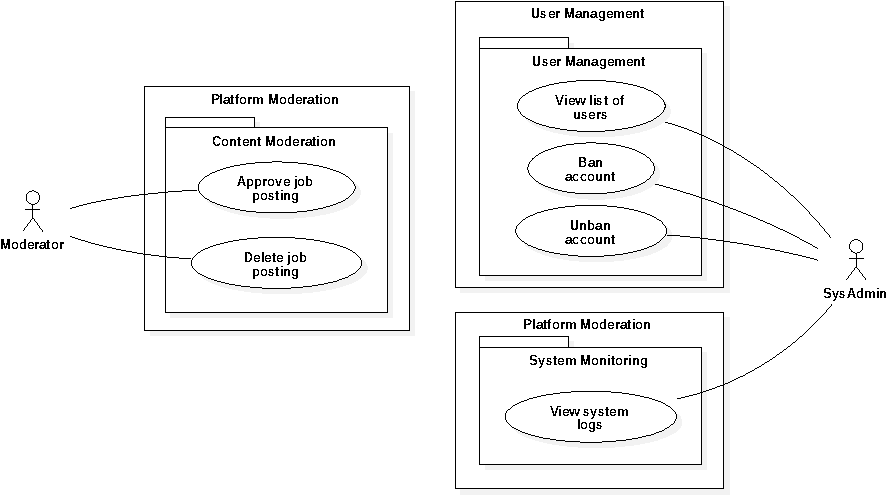
\includegraphics[width=\linewidth]{diagrams/exported/Use Case/Use-Case-Back Office-crop.pdf}
	\caption{Back Office Worker Use Case Diagram.}
	\label{diagram:uc-back_office}
\end{figure}

Unlike Job Seekers and Employers, the Back Office Workers primarily performs supervisory tasks highlighted in Figure \ref{diagram:uc-back_office}. These include user management, moderation of job postings, and maintaining the overall quality and security of the platform.


\chapter{Supplementary Use Case Specifications}
\label{appendix:supplementary-usecase-specs}

\section{Guest: Login}

\begin{usecasespectable}
	{Use Case Specification: Login.}
	{tab:ucs-login}

	Use Case ID & UC-AUTH-02 \\ \hline

	Use Case Name & Login \\ \hline

	Primary Actor & Guest \\ \hline

	Description &
	Allows a guest to authenticate using registered credentials and become an authenticated user.
	\\ \hline

	Goal &
	Authenticate a registered user and grant access to protected system functions.
	\\ \hline

	Preconditions &
	\begin{itemize}
		\item The user has a registered account.
		\item The user is not currently authenticated.
	\end{itemize}
	\\ \hline

	Trigger &
	The user clicks "Log In" button from the website's header
	\\ \hline

	Main Success Scenario &
	\begin{enumerate}
		\item Guest selects "Login".
		\item System displays the login form.
		\item Guest enters email and password.
		\item Guest submits the login form.
		\item System validates the submitted credentials.
		\item System authenticates the user.
		\item System establishes an authenticated session.
		\item System redirects the user to the authenticated homepage.
		\item System displays a successful login message.
	\end{enumerate}
	\\ \hline

	Alternative Flows &
	\textbf{A1. Invalid credentials}
	\begin{enumerate}
		\item The system reports the error "Invalid email or password".
	\end{enumerate}

	\textbf{A2. Invalid email address}
	\begin{enumerate}
		\item The system reports the error "Invalid email".
	\end{enumerate}

	\textbf{A3. Missing required input fields}
	\begin{enumerate}
		\item The system reports the error "Please fill out required fields".
	\end{enumerate}

	\textbf{A4. Account is suspended}
	\begin{enumerate}
		\item System denies authentication.
		\item System informs the user that the account has been suspended.
	\end{enumerate}
	\\ \hline

	Postconditions &
	\begin{itemize}
		\item The user is successfully authenticated.
		\item The user gains access to functions available to authenticated users.
	\end{itemize}
	\\ \hline

\end{usecasespectable}

\section{Authenticated User: Update Personal Information}

\begin{usecasespectable}
	{Use Case Specification: Update Personal Information.}
	{tab:ucs-update_personal_information}

	Use Case ID & UC-PROFILE-01 \\ \hline

	Use Case Name & Update Personal Information \\ \hline

	Primary Actor & Authenticated User \\ \hline

	Goal & Maintain accurate personal information within the platform. \\ \hline

	Description &
	Allows an authenticated user to update personal profile information.
	\\ \hline

	Preconditions &
	\begin{itemize}
		\item User is authenticated.
	\end{itemize}
	\\ \hline

	Trigger &
	The user selects the Profile page.
	\\ \hline

	Main Success Scenario &
	\begin{enumerate}
		\item User opens the profile page.
		\item System displays current profile information.
		\item User edits profile information.
		\item User submits the changes.
		\item System validates the submitted information.
		\item System updates the profile.
		\item System confirms the successful update.
	\end{enumerate}
	\\ \hline

	Alternative Flows &
	\textbf{A1. Invalid input}
	\begin{enumerate}
		\item System highlights invalid fields.
		\item User corrects the information.
	\end{enumerate}
	\\ \hline

	Postconditions &
	\begin{itemize}
		\item Updated profile information is stored.
	\end{itemize}
	\\ \hline

\end{usecasespectable}

\section{Back Office Worker: Approve Job Posting}

\begin{usecasespectable}
	{Use Case Specification: Approve Job Posting.}
	{tab:ucs-approve_job_posting}

	Use Case ID & UC-ADMIN-01 \\ \hline

	Use Case Name & Approve Job Posting \\ \hline

	Primary Actor & Back Office Worker \\ \hline

	Goal & Review and approve job postings before they become publicly available. \\ \hline

	Description &
	Allows a Back Office Worker to review submitted job postings and determine whether they comply with platform policies.
	\\ \hline

	Preconditions &
	\begin{itemize}
		\item Back Office Worker is authenticated.
		\item A job posting is awaiting approval.
	\end{itemize}
	\\ \hline

	Trigger &
	Administrator opens the pending job posting list.
	\\ \hline

	Main Success Scenario &
	\begin{enumerate}
		\item Back Office Worker reviews the job posting.
		\item Back Office Worker verifies the submitted information.
		\item Back Office Worker approves the posting.
		\item System updates the posting status.
		\item System makes the job posting publicly available.
	\end{enumerate}
	\\ \hline

	Alternative Flows &
	\textbf{A1. Job posting rejected}
	\begin{enumerate}
		\item Administrator rejects the posting.
		\item System records the decision.
		\item System notifies the Employer.
	\end{enumerate}
	\\ \hline

	Postconditions &
	\begin{itemize}
		\item The job posting is approved or rejected.
	\end{itemize}
	\\ \hline

\end{usecasespectable}


\chapter{Supplementary Entity Relationship Groups}
\label{appendix:supplementary-erd}

The entity relationship groups that support the remaining modules are detailed here for reference.

\section{Auth and Account}

Figure~\ref{diagram:erd-auth-account} details the entities involved in authentication and account recovery.

\begin{figure}[H]
	\centering
	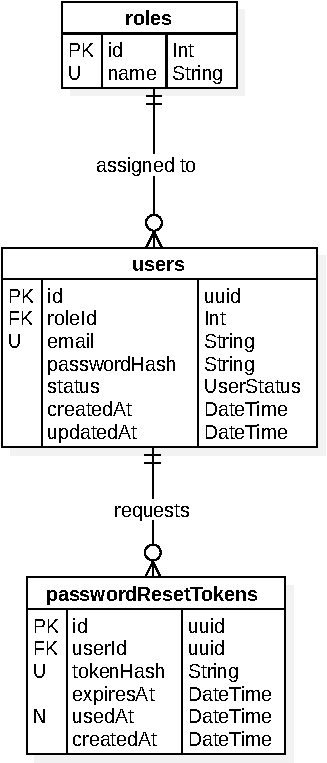
\includegraphics[width=0.32\linewidth]{diagrams/exported/ERD/Auth-and-Account-ERD-crop.pdf}
	\caption{Auth and Account Entity Relationship Diagram.}
	\label{diagram:erd-auth-account}
\end{figure}

Each role may be assigned to any number of users, while every user is assigned exactly one role. A user may request multiple password reset tokens over time, but each token belongs to exactly one user.

\section{Profile and CV Management}

Figure~\ref{diagram:erd-profile-cv} details the entities involved in managing a user's profile, job preferences, and resumes.

\begin{figure}[H]
	\centering
	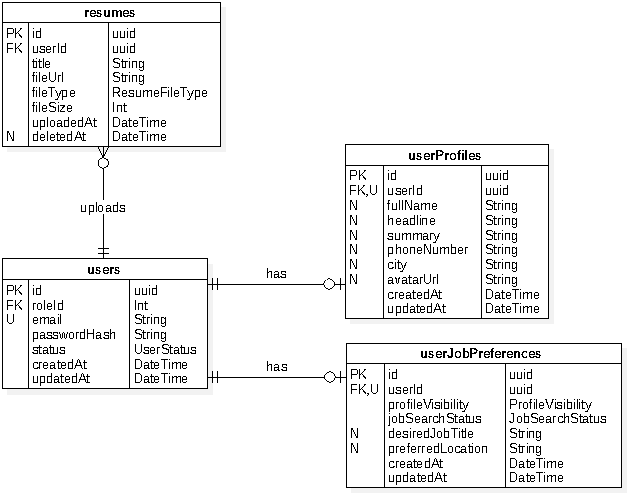
\includegraphics[width=\linewidth]{diagrams/exported/ERD/Profile-and-CV-Management-ERD-crop.pdf}
	\caption{Profile and CV Management Entity Relationship Diagram.}
	\label{diagram:erd-profile-cv}
\end{figure}

Each user has at most one profile and at most one job preference record, both enforced through a unique foreign key, forming one-to-one relationships. A user may upload multiple resumes, but each resume belongs to exactly one user.

\section{Administration and Audit}

Figure~\ref{diagram:erd-admin-audit} details the entities involved in role assignment and system activity logging.

\begin{figure}[H]
	\centering
	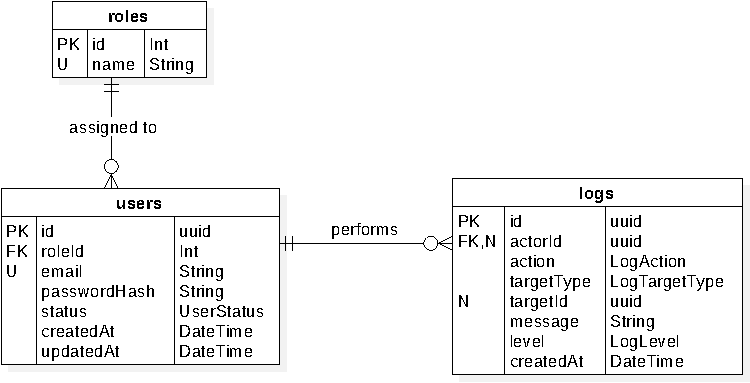
\includegraphics[width=\linewidth]{diagrams/exported/ERD/Administration-and-Audit-ERD-crop.pdf}
	\caption{Administration and Audit Entity Relationship Diagram.}
	\label{diagram:erd-admin-audit}
\end{figure}

As with the Auth and Account group, each role may be assigned to any number of users, while every user is assigned exactly one role. A user may perform any number of logged actions, and each log entry optionally references the user who performed it, since some actions may be attributed to the system itself rather than a specific user.


\chapter{Supplementary Module Designs}
\label{appendix:supplementary-design}

This chapter collects the class-level design of the modules that are not featured in the main body. Each module follows the same controller--service pattern described in Chapter \ref{chapter:system-design}; as with the featured modules, each Controller delegates directly to its Service, which owns all business logic and Prisma access.

\section{Authentication Module}

The Authentication Module implements user registration, login, logout, and password recovery. It resides in \texttt{api-external}, since these operations are invoked directly by external clients, and is the module other modules depend on for issuing and validating access tokens.

Figure~\ref{diagram:class-auth} presents the class diagram of the Authentication Module.

\begin{figure}[H]
	\centering
	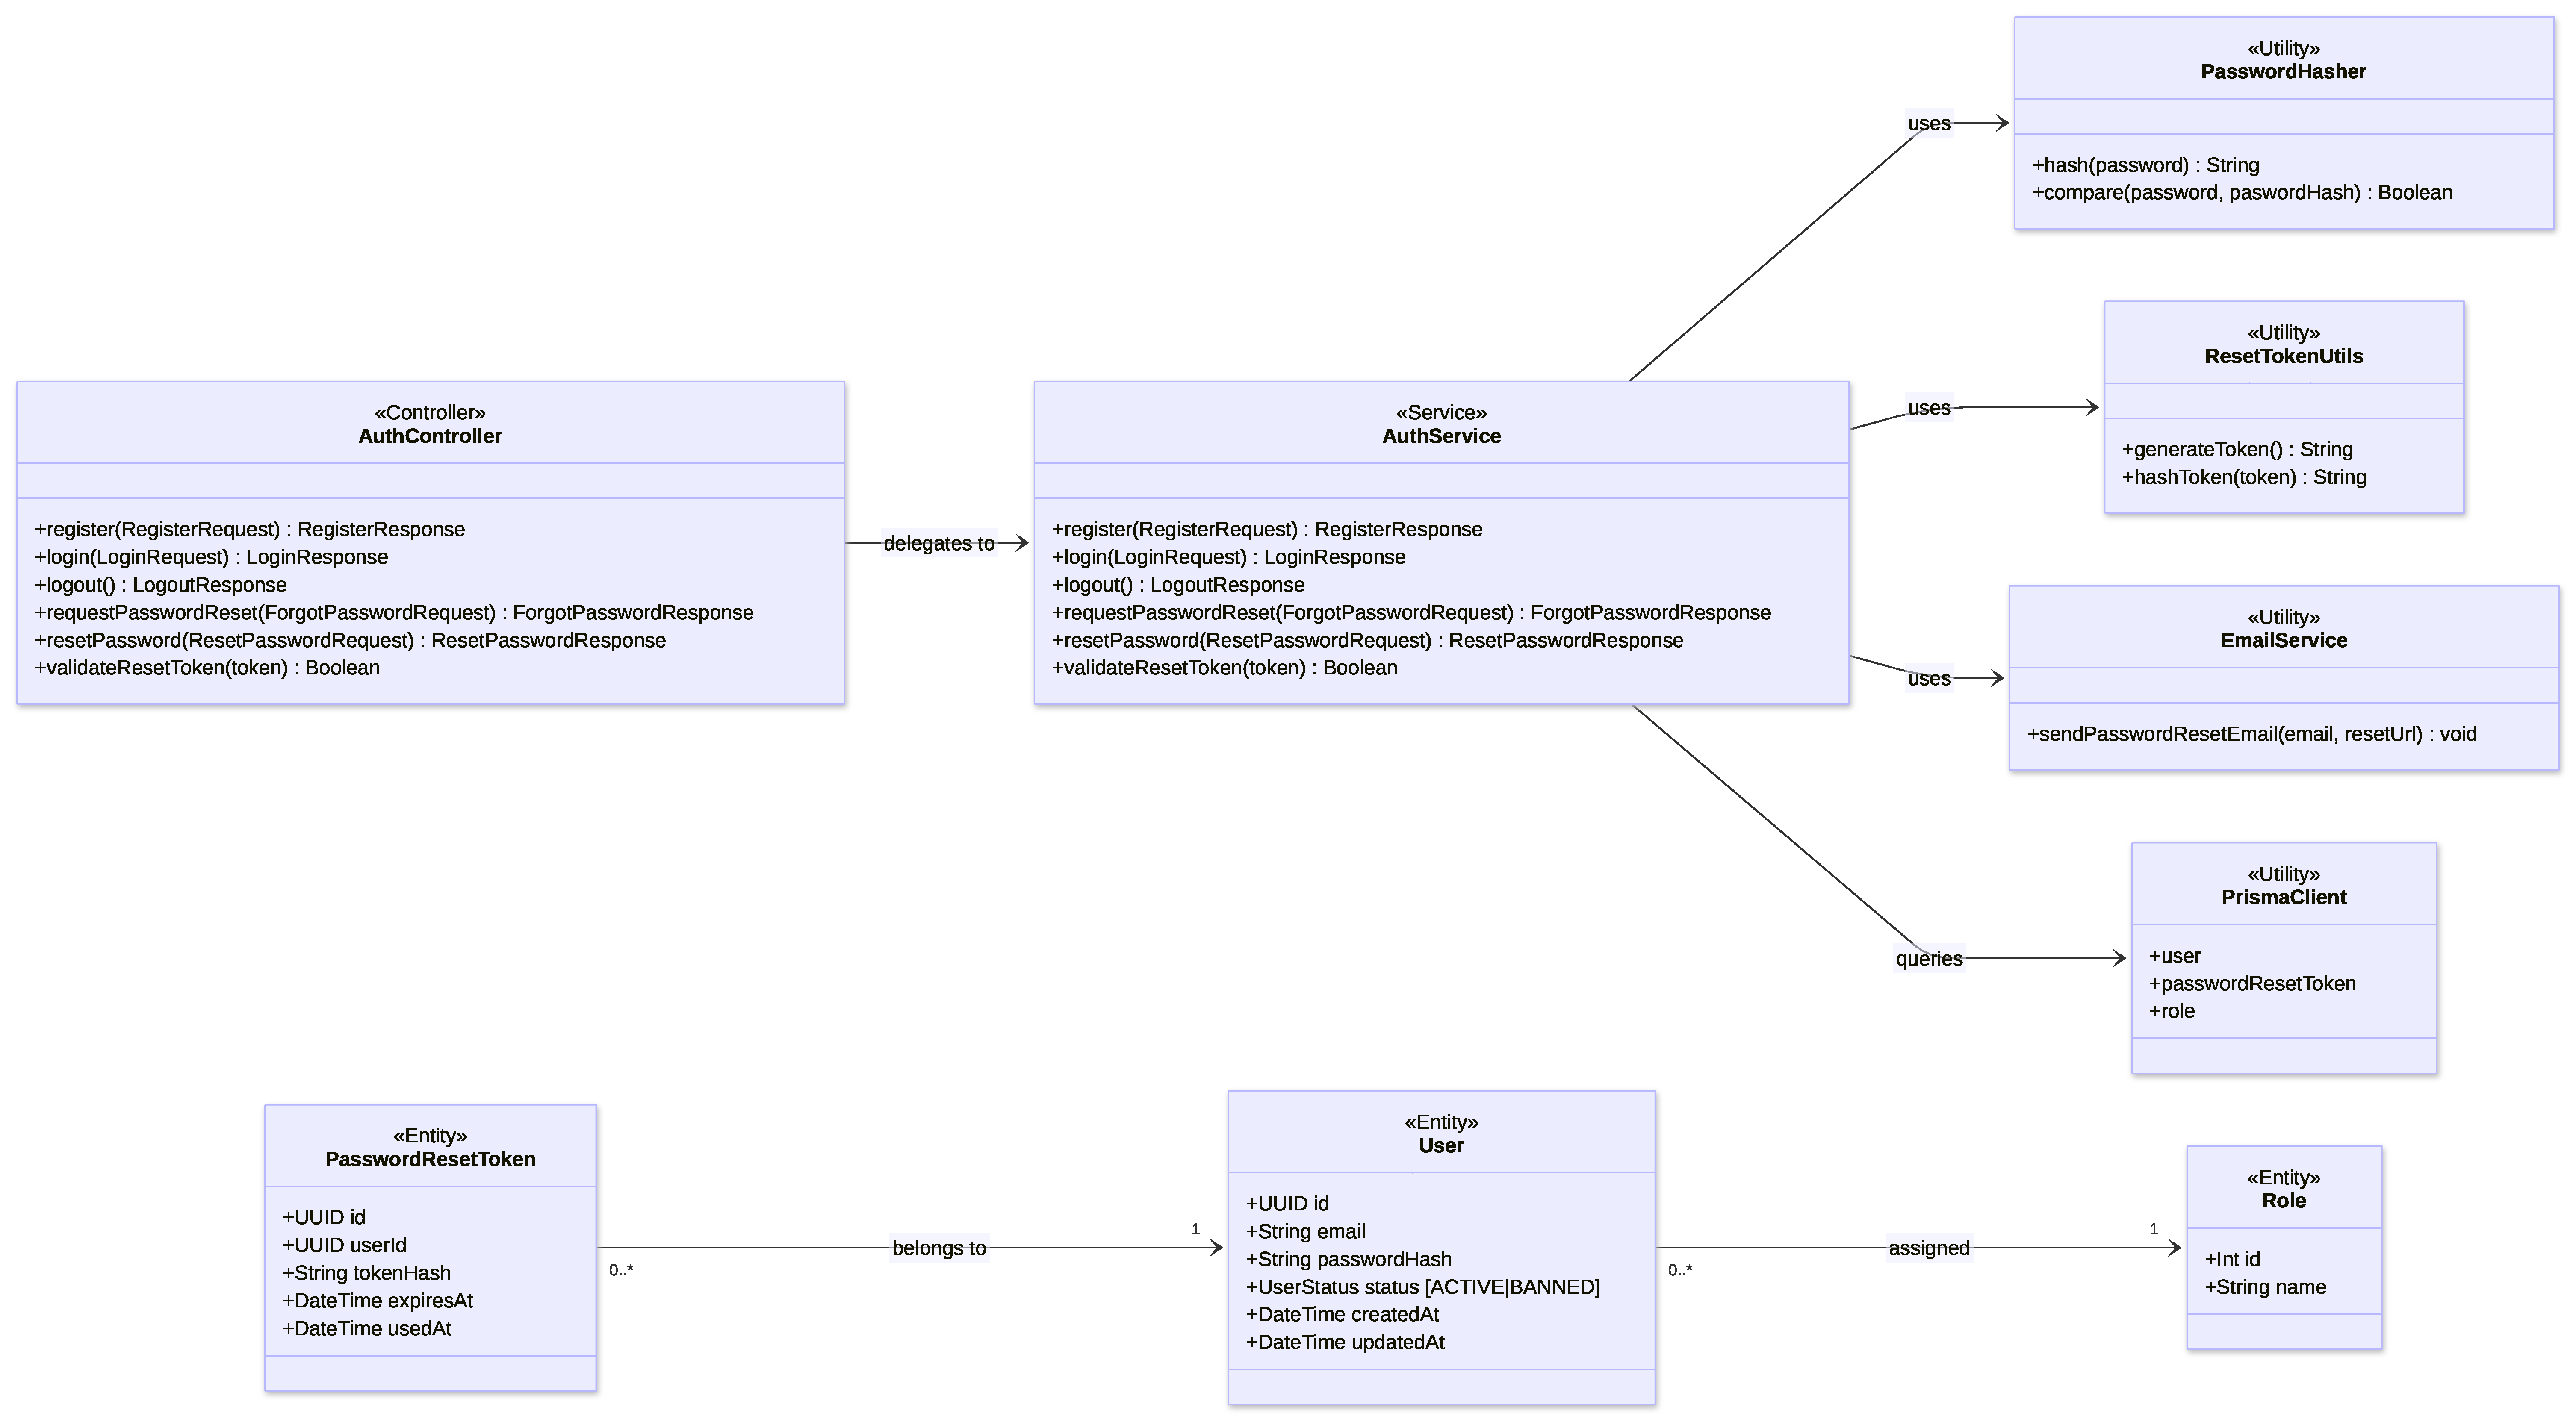
\includegraphics[width=\linewidth]{diagrams/exported/2Auth/Auth-Class-Diagram.pdf}
	\caption{Authentication Module Class Diagram.}
	\label{diagram:class-auth}
\end{figure}

AuthController exposes the authentication endpoints and delegates each directly to a matching method on AuthService. AuthService depends on the shared utility components: PasswordHasher, ResetTokenUtils, EmailService, and Prisma Client. Each AuthService method implements one authentication use case. register validates that the email is not already in use, assigns the default \texttt{JOB\_SEEKER} role, and stores the hashed password. login verifies the submitted password against the stored hash, rejects banned accounts, and issues a signed JWT containing the user's identifier and role. logout returns a simple confirmation message, since JWTs are stateless and token discarding is handled by the frontend. requestPasswordReset issues a hashed, time-limited reset token and emails the corresponding raw token to the user; the same response is returned whether or not the account exists, so the email address is not revealed. resetPassword validates the submitted token against the stored hash and expiration, then updates the password and marks the token as used within a single transaction. validateResetToken lets the frontend check whether a reset token is still valid without consuming it.

\section{Profile Management Module}

The Profile Management Module lets authenticated users view and update their personal profile, job search preferences, avatar, and account password. It resides in \texttt{api-external} and depends on the JWT middleware to identify the requesting user on every operation.

Figure~\ref{diagram:class-profile} presents the class diagram of the Profile Management Module.

\begin{figure}[H]
	\centering
	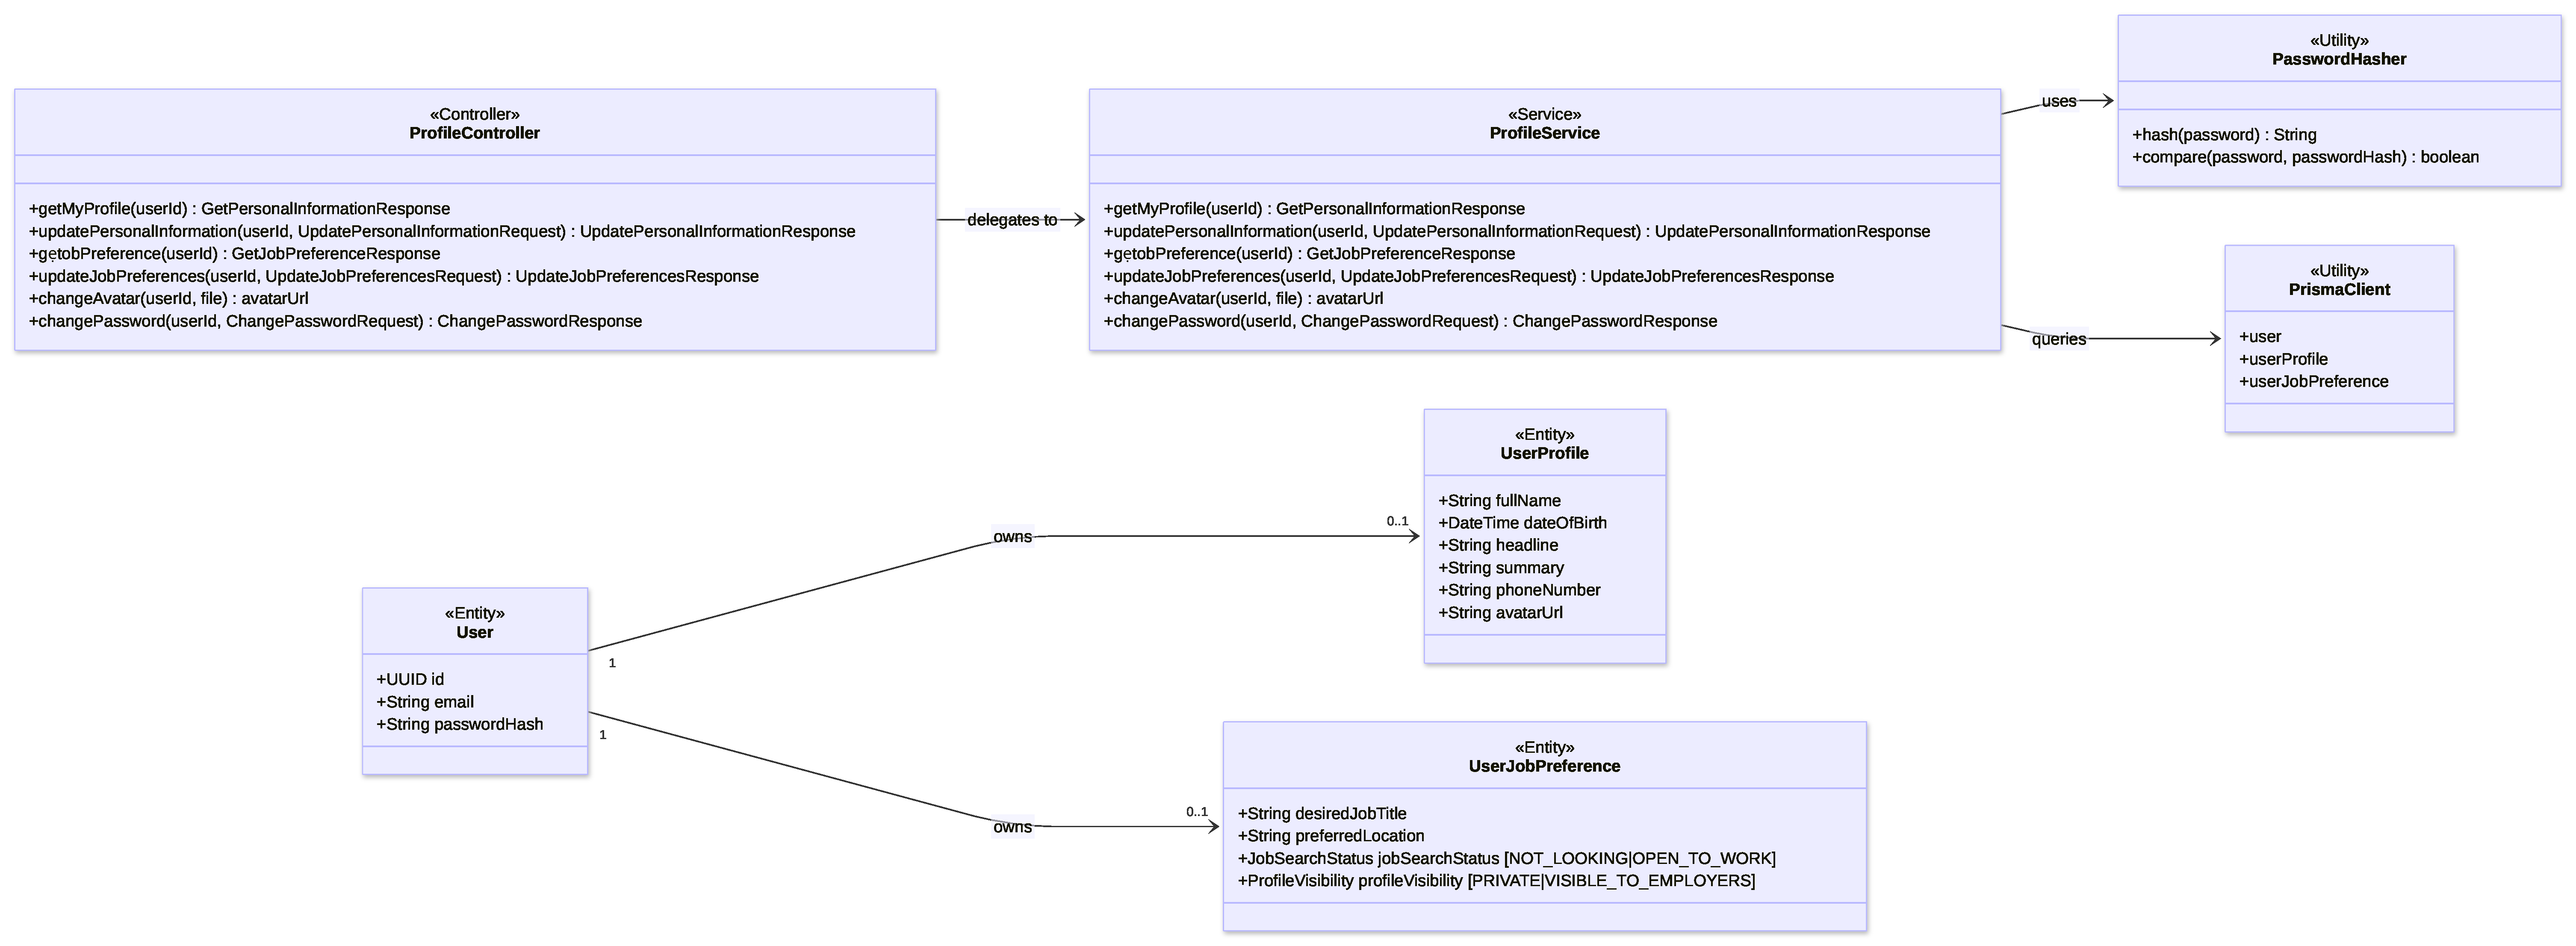
\includegraphics[width=\linewidth]{diagrams/exported/3Profile/Profile-Class-Diagram.pdf}
	\caption{Profile Management Module Class Diagram.}
	\label{diagram:class-profile}
\end{figure}

ProfileController delegates each of its endpoints directly to a method on ProfileService. ProfileService depends on PasswordHasher, FileStorageService, and Prisma Client. getMyProfile and getJobPreference return the authenticated user's records, selecting only fields safe for display. updatePersonalInformation and updateJobPreference use an upsert operation, creating the record on first use and updating it thereafter; updateJobPreference additionally distinguishes an omitted field (left unchanged) from a field explicitly set to \texttt{null} (cleared). changeAvatar validates the uploaded file's type and size before storing it. changePassword verifies the submitted current password, rejects the request if the new password is identical to the old one, and otherwise hashes and stores the new password.

\section{Resume Management Module}

The Resume Management Module lets job seekers list, upload, and delete their resumes, which are later selected when submitting job applications. It resides in \texttt{api-external} and depends on the JWT middleware.

Figure~\ref{diagram:class-resume} presents the class diagram of the Resume Management Module.

\begin{figure}[H]
	\centering
	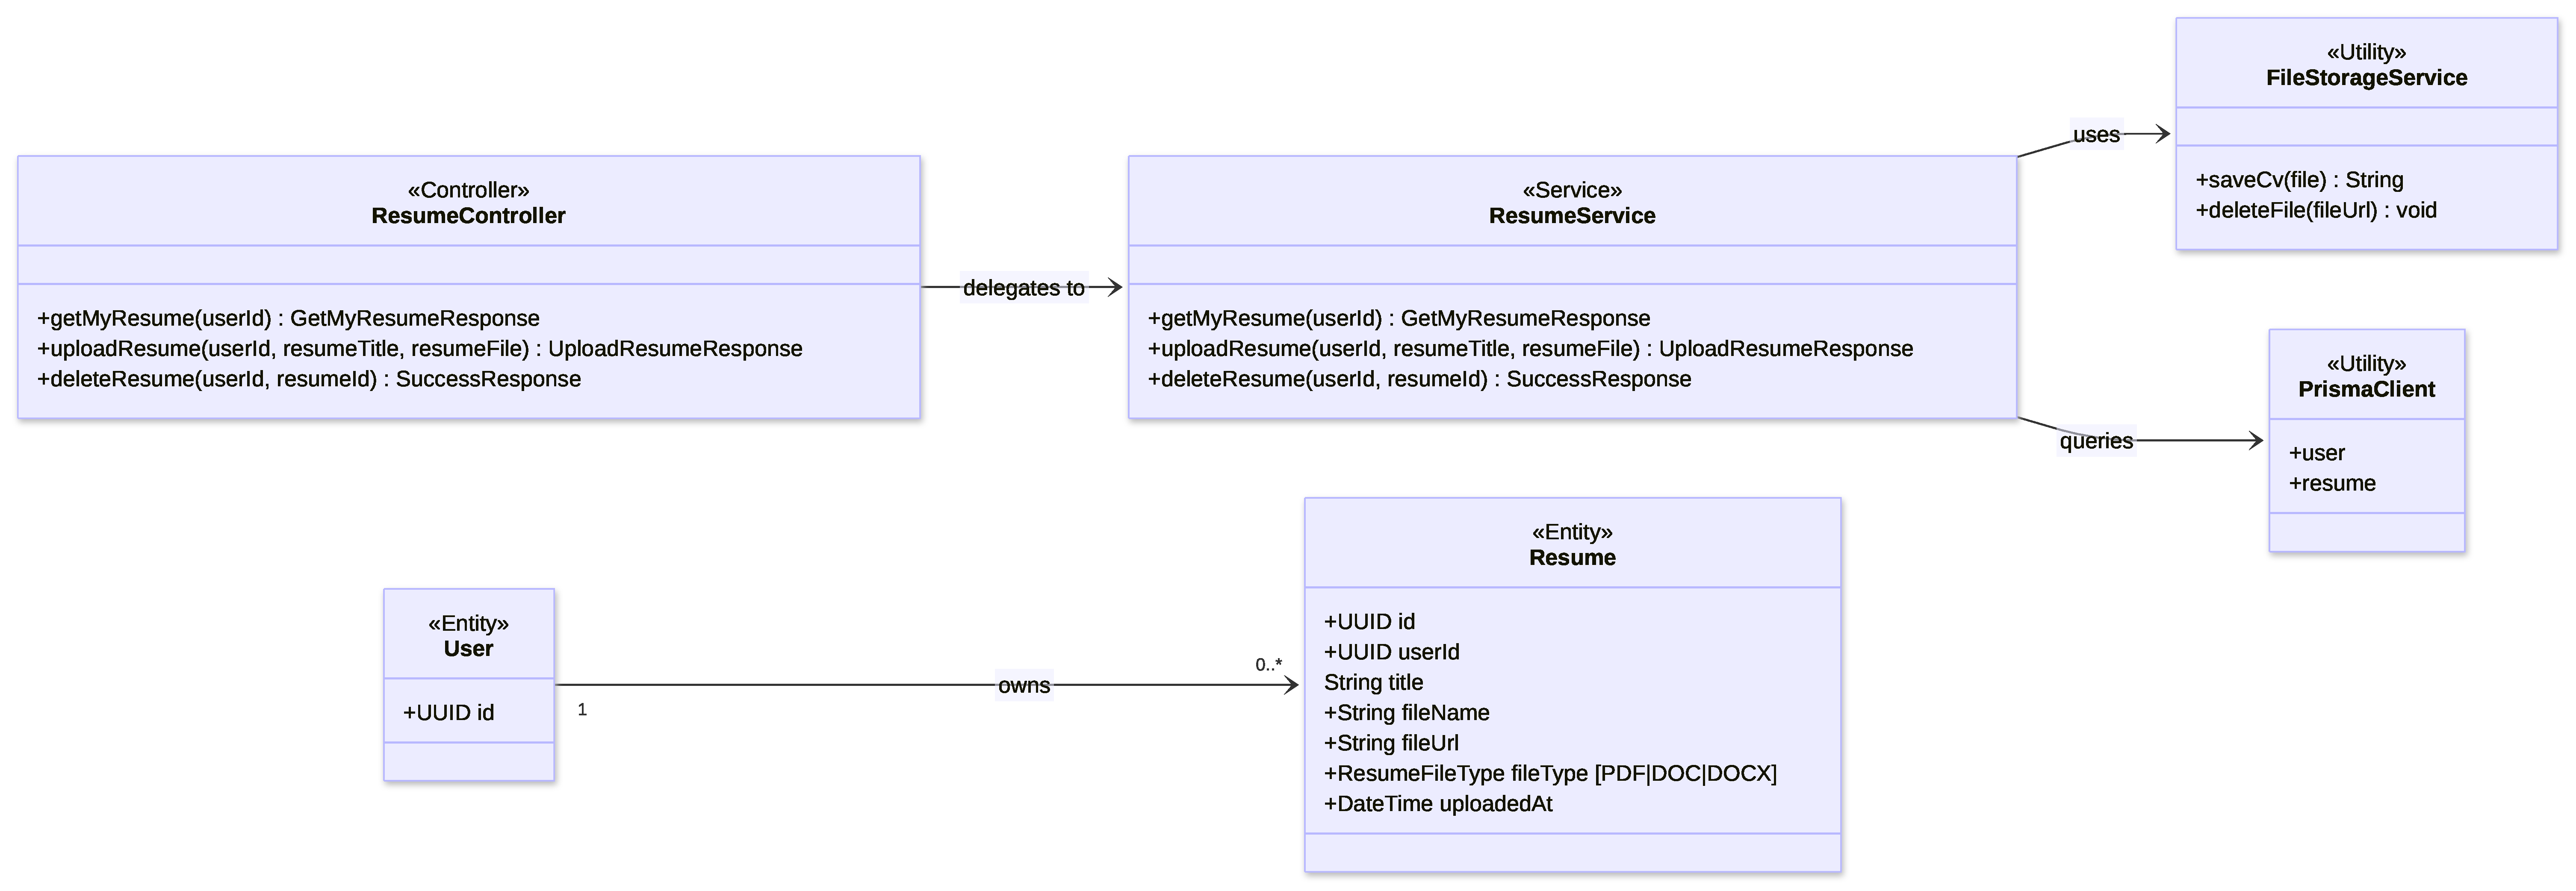
\includegraphics[width=\linewidth]{diagrams/exported/4Resume/Resume-Class-Diagram.pdf}
	\caption{Resume Management Module Class Diagram.}
	\label{diagram:class-resume}
\end{figure}

ResumeController delegates its endpoints to ResumeService, which depends on FileStorageService and Prisma Client. getMyResumes returns the authenticated user's non-deleted resumes, ordered from newest to oldest. uploadResume validates that a title and file are provided, rejects files larger than 5~MB or of an unsupported type (only PDF, DOC, and DOCX are accepted), stores the file through FileStorageService, then creates the resume record. deleteResume verifies that the resume exists, is not already deleted, and belongs to the requesting user, then checks whether it is referenced by any application. If it is, the resume is soft-deleted so existing applications retain a valid reference; otherwise it is hard-deleted from both the database and file storage.

\section{Job Discovery Module}

The Job Discovery Module lets guests and authenticated users search active job postings and view their details. Unlike the previous modules, its endpoints are not protected by the JWT middleware, since job browsing is a public capability. It also includes the public-facing company profile and active job listing endpoints operated by \texttt{CompanyController} and \texttt{CompanyService}.

Figure~\ref{diagram:class-job-discovery} presents the Public class diagram, which covers both the job discovery and company profile viewing capabilities.

\begin{figure}[H]
	\centering
	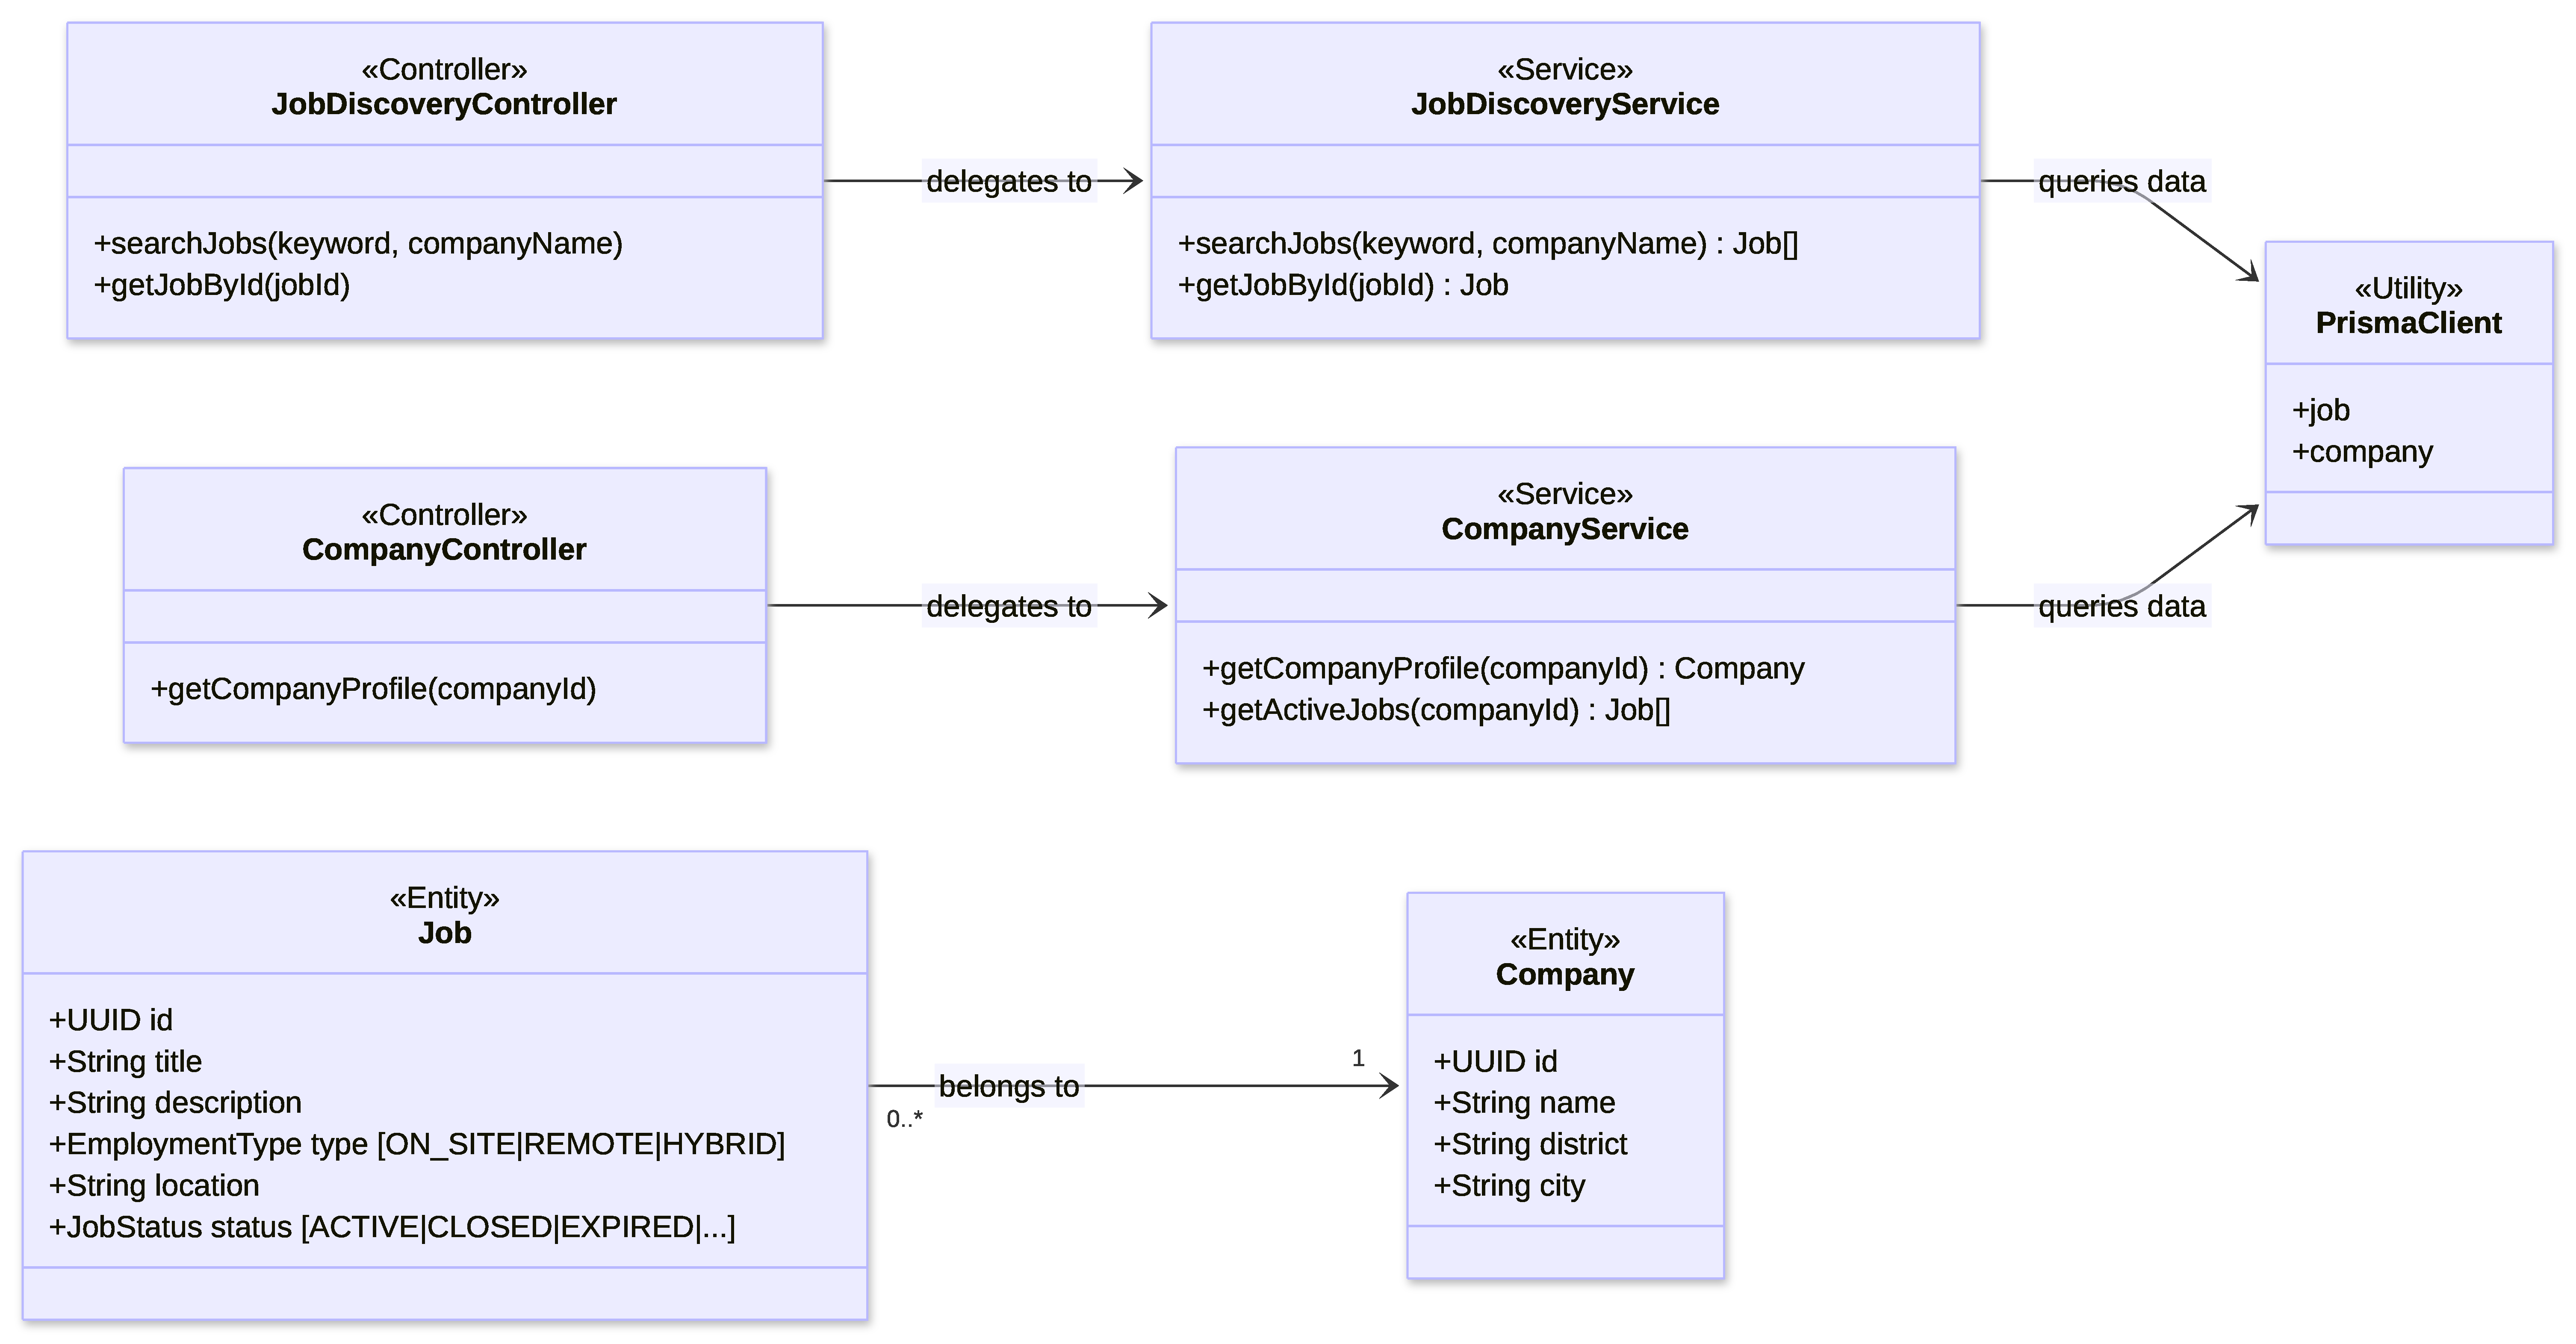
\includegraphics[width=\linewidth]{diagrams/exported/1Public/Public-Class-Diagram.pdf}
	\caption{Public Class Diagram.}
	\label{diagram:class-job-discovery}
\end{figure}

JobDiscoveryService depends on the shared Prisma Client, which queries the Job and Company entities. searchJobs restricts results to \texttt{ACTIVE} jobs and accepts an optional keyword and location, either of which may be provided independently or together. An empty string is treated as not provided, each value is capped at 255 characters, and the keyword matches against the job title or company name while the location matches against the job location or the company's city and district, case-insensitively. Neither is required: if no keyword is given, all active jobs are returned, and a query that matches nothing returns an empty list rather than an error. getJobDetail returns the full detail of a single active job by identifier, with a 404 error if the job does not exist or is not currently active.

\section{Back Office Module}

The Back Office module is hosted under \texttt{api-internal}. Figure~\ref{diagram:class-back-office} presents its class diagram.

\begin{figure}[H]
	\centering
	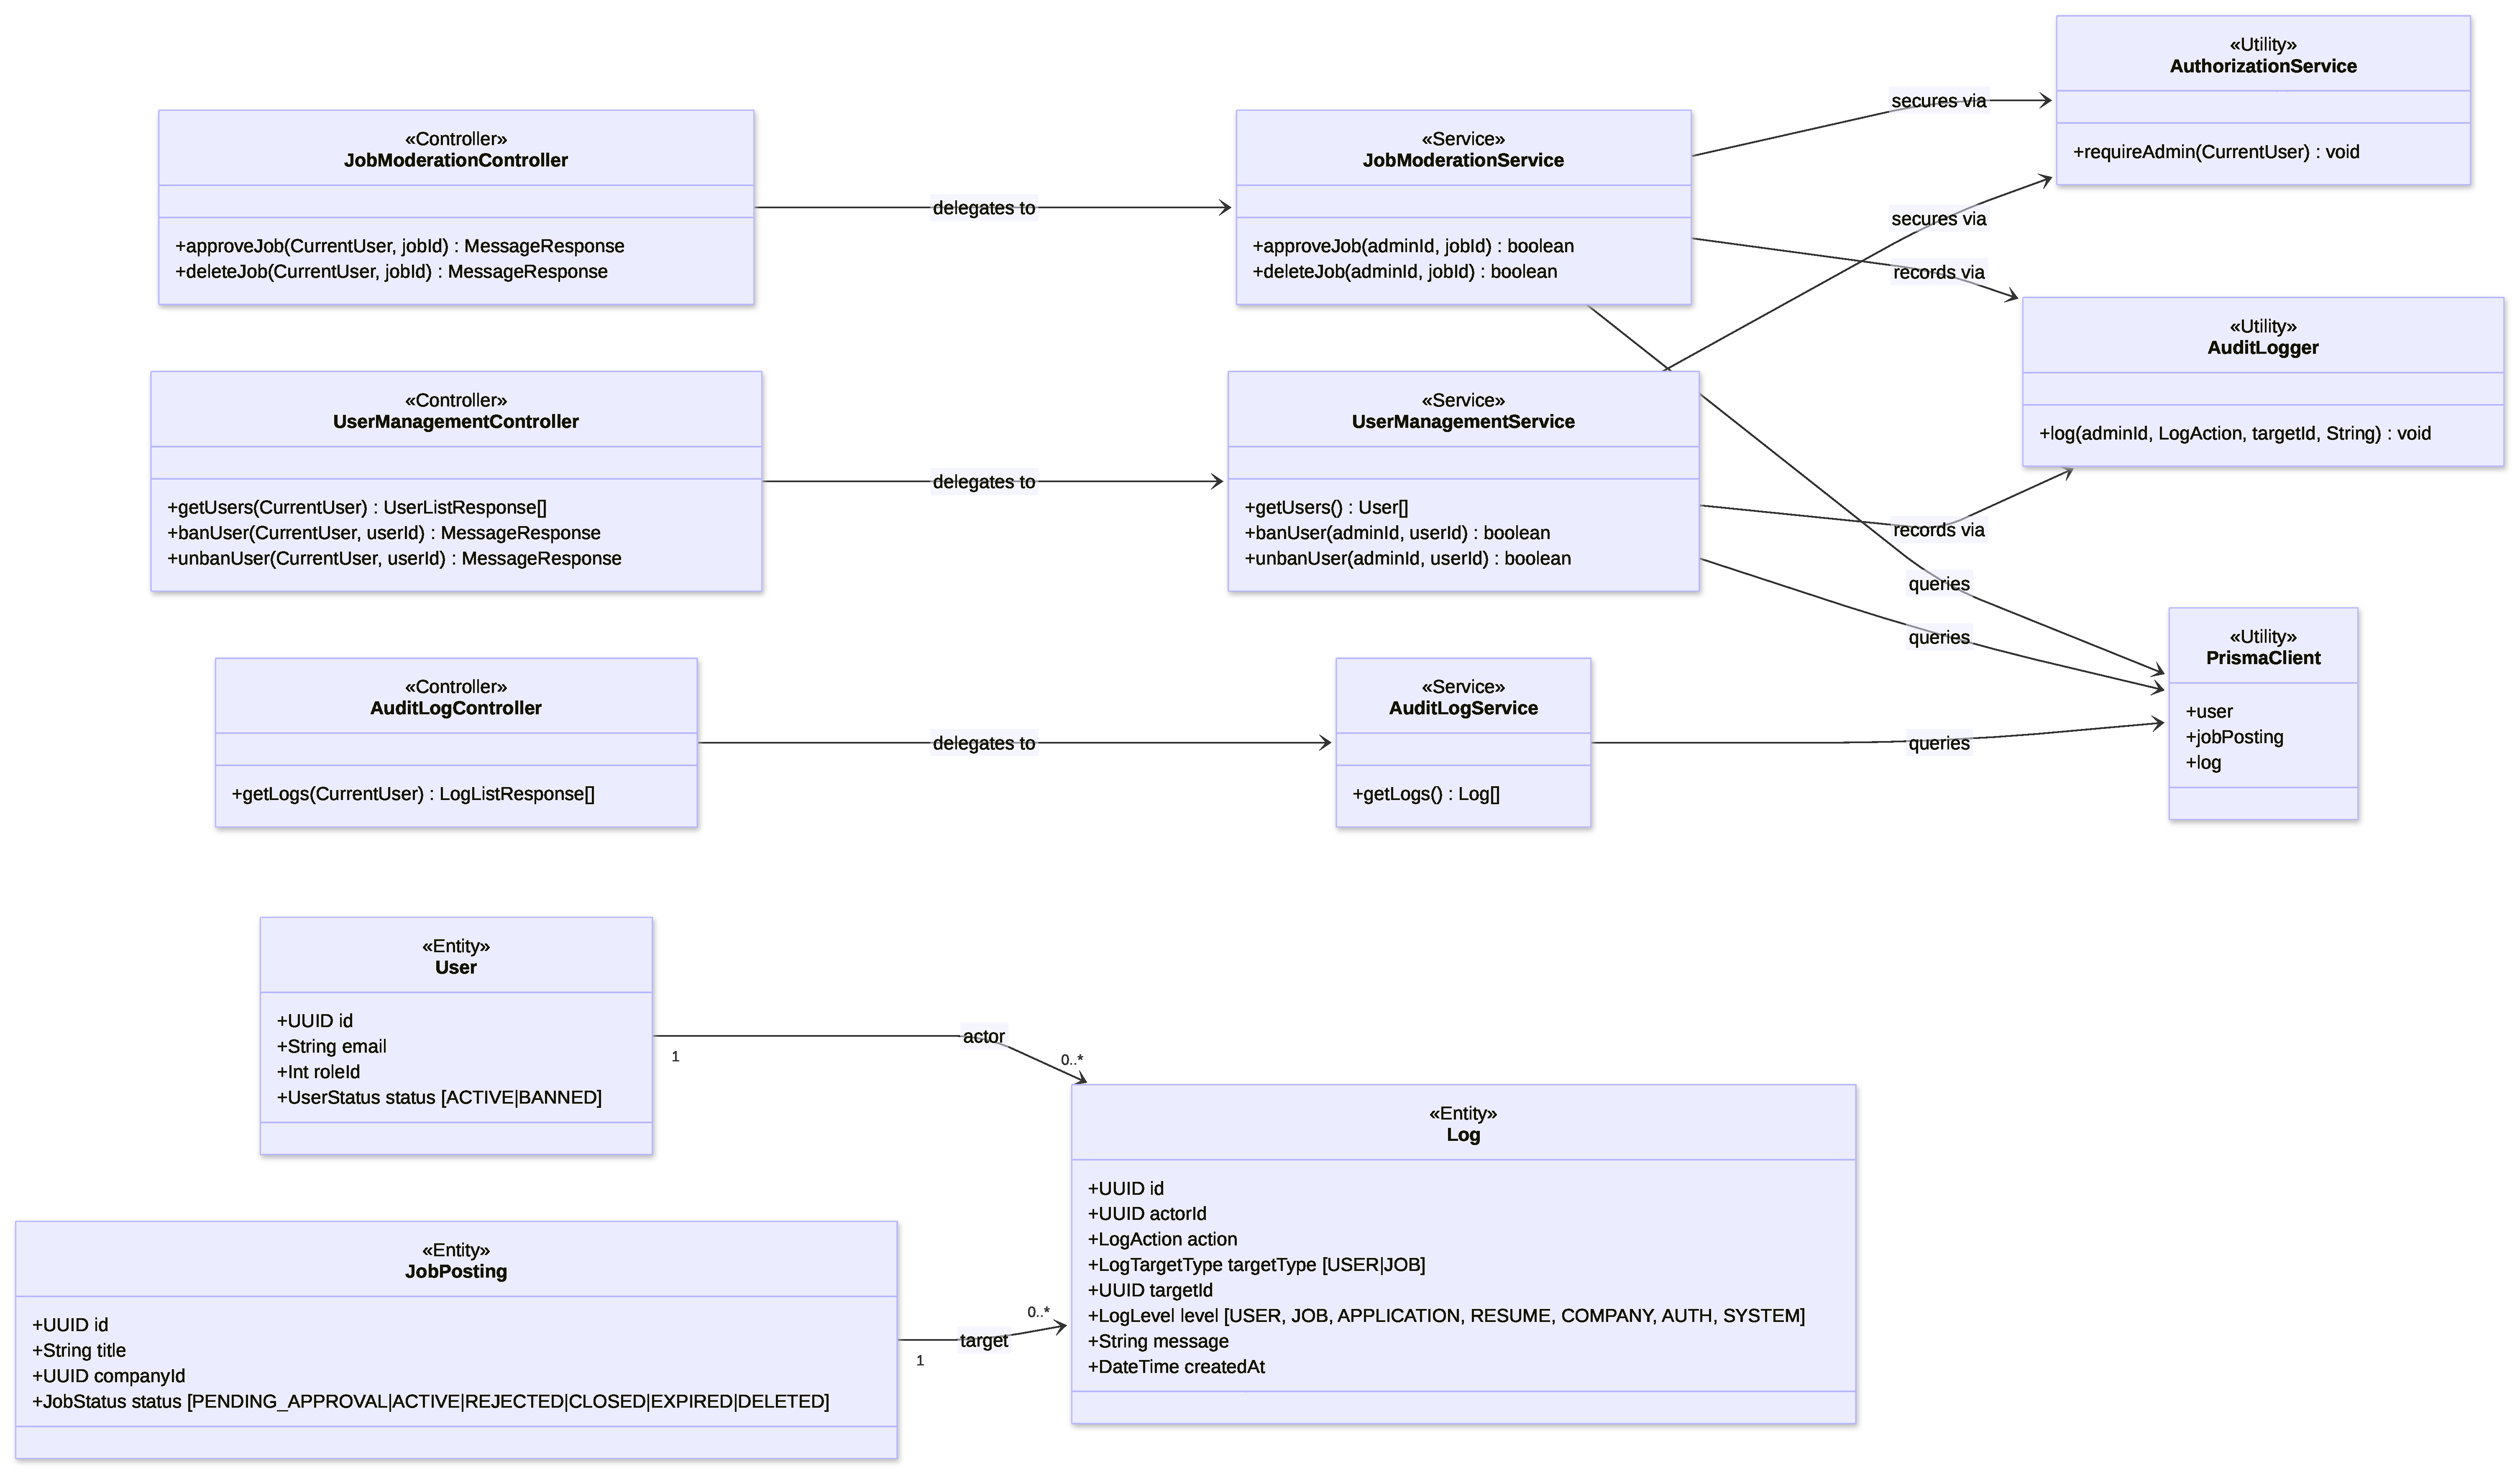
\includegraphics[width=\linewidth]{diagrams/exported/7BackOffice/BackOffice-Class-Diagram.pdf}
	\caption{Back Office Class Diagram.}
	\label{diagram:class-back-office}
\end{figure}


\chapter{Sequence Diagrams}
\label{appendix:sequence-diagrams}

This chapter collects the sequence diagrams of the platform's use cases as reference material. They illustrate the interaction between the actor, the frontend, and the backend service for each flow, and supplement the design discussion in Chapter \ref{chapter:system-design} and the implementation discussion in Chapter \ref{chapter:implementation}.

\section{Job Application}

\begin{figure}[H]
	\centering
	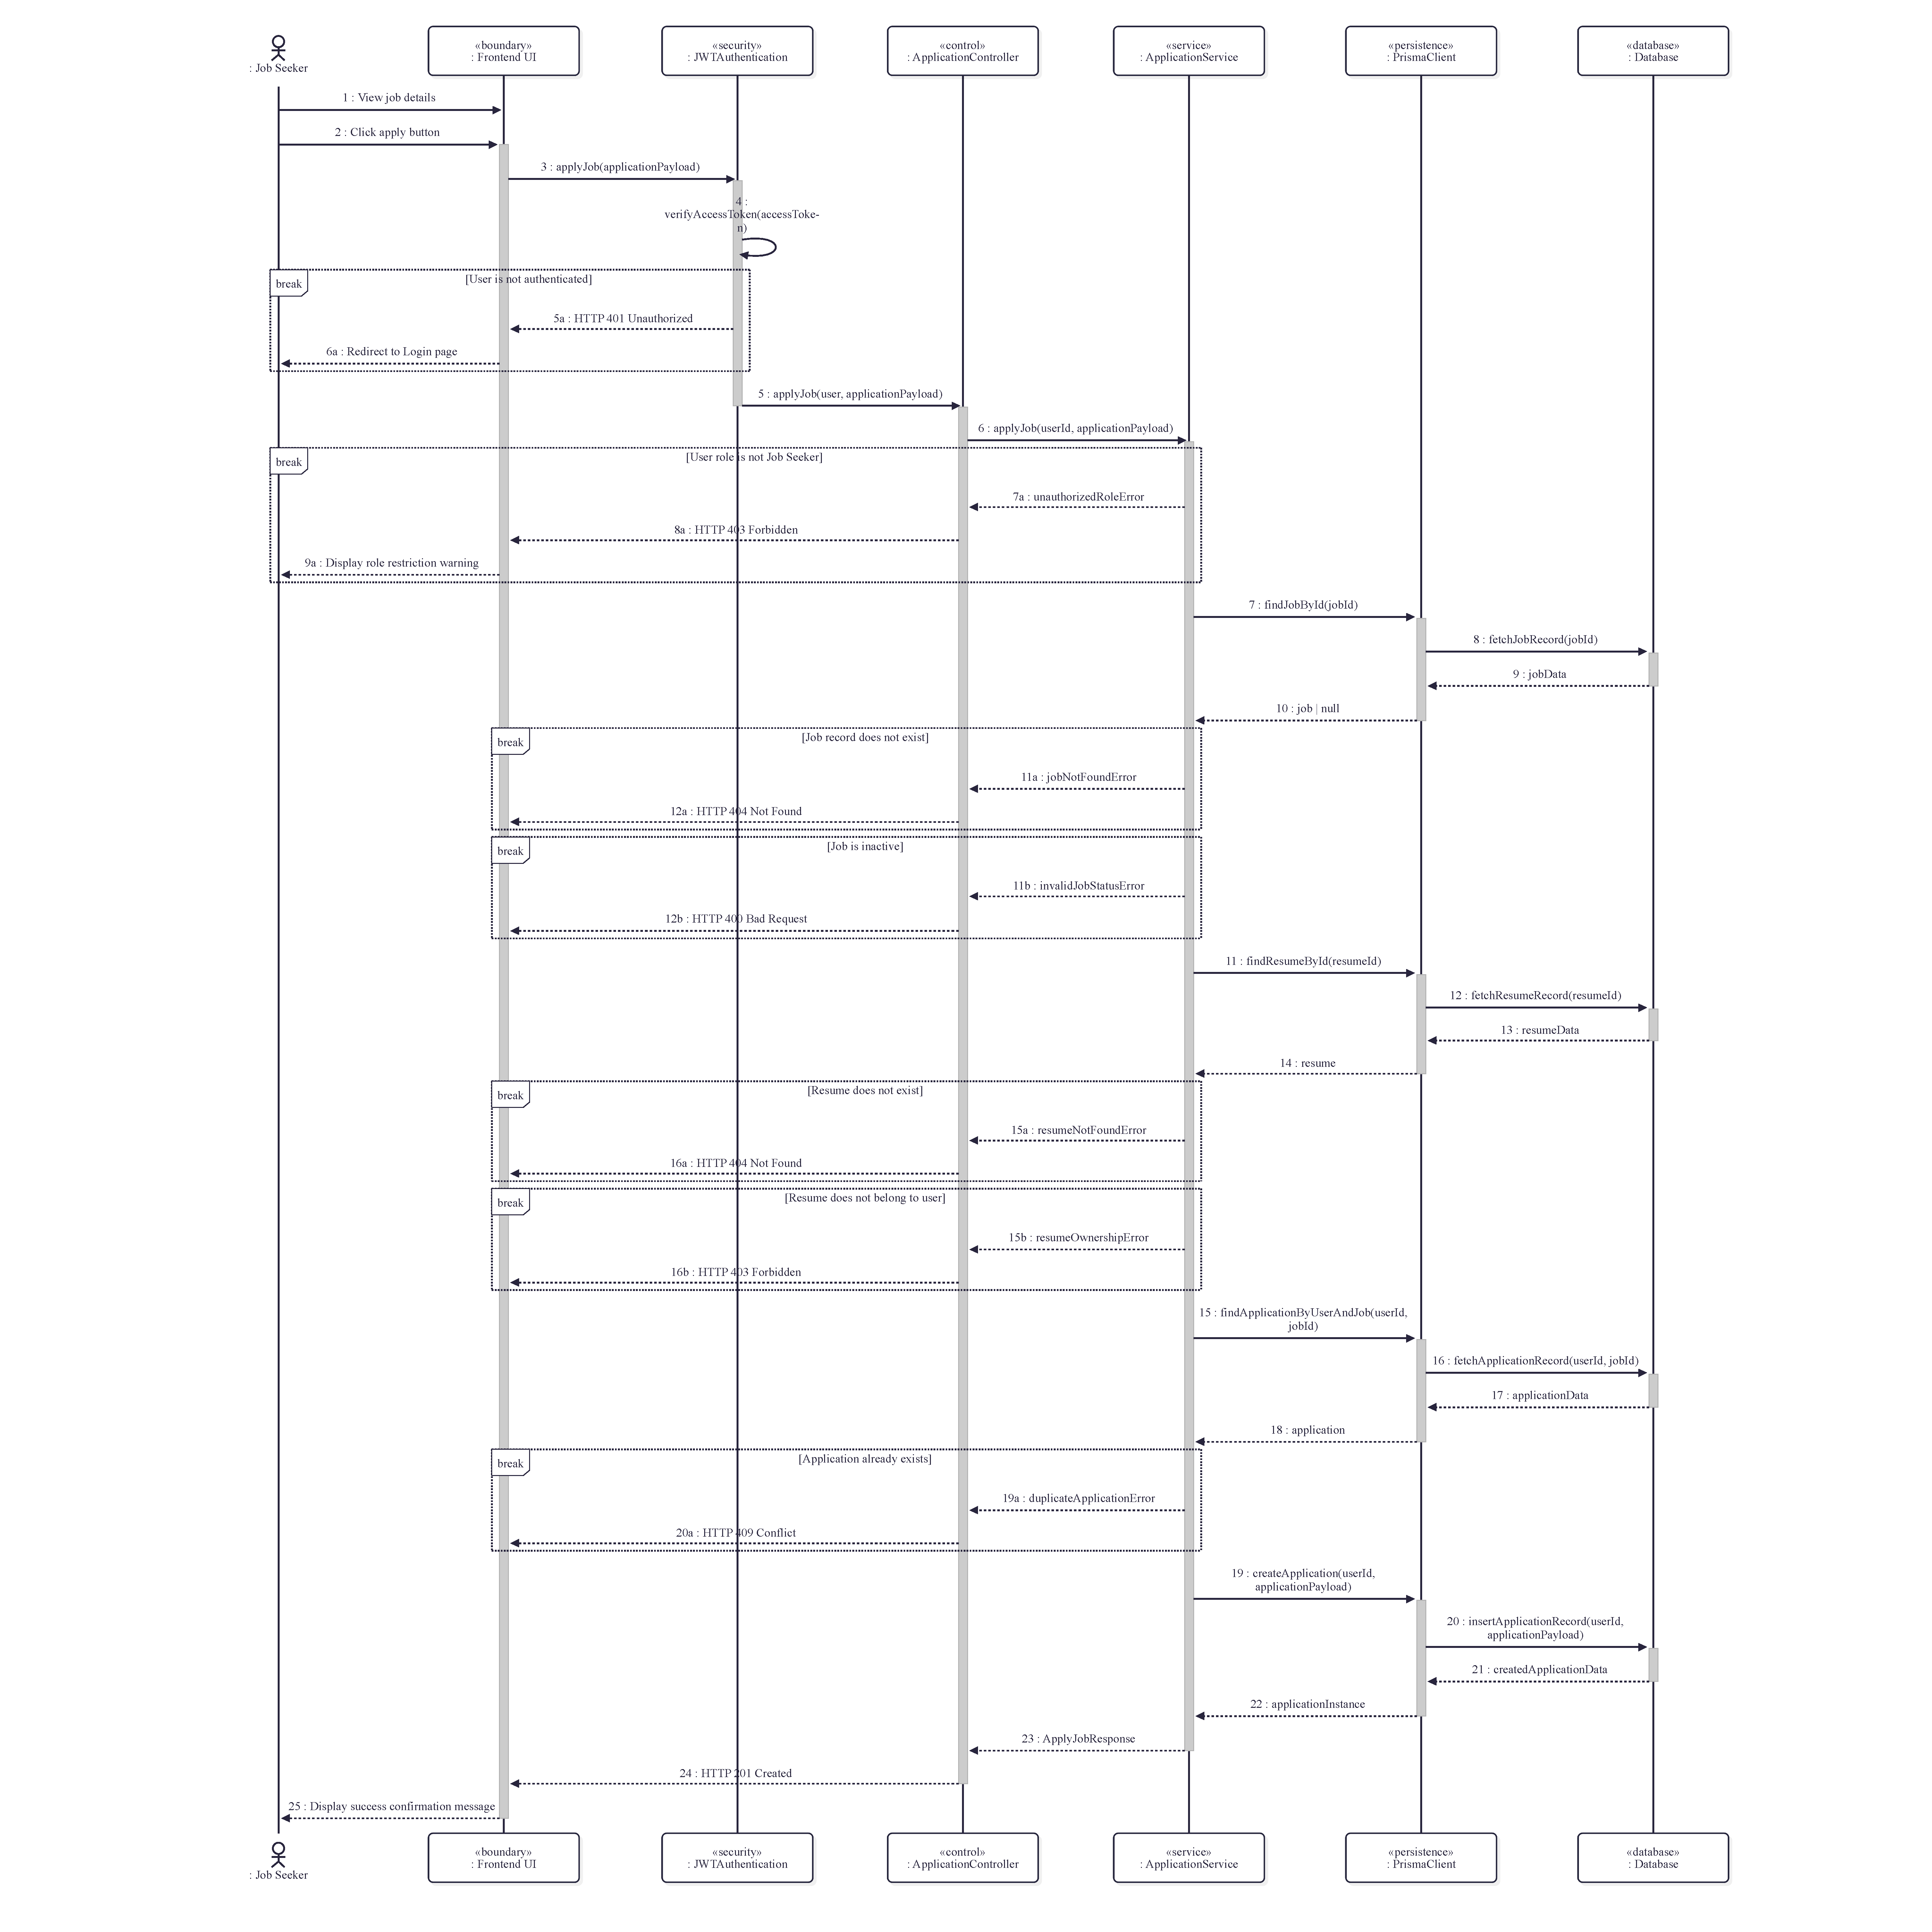
\includegraphics[width=0.9\linewidth]{diagrams/exported/5JobSeeker/SD-JobSeeker01-Apply-For-Jobs.pdf}
	\caption{Sequence Diagram: Apply for Jobs.}
	\label{diagram:sd-jobseeker-apply}
\end{figure}

\begin{figure}[H]
	\centering
	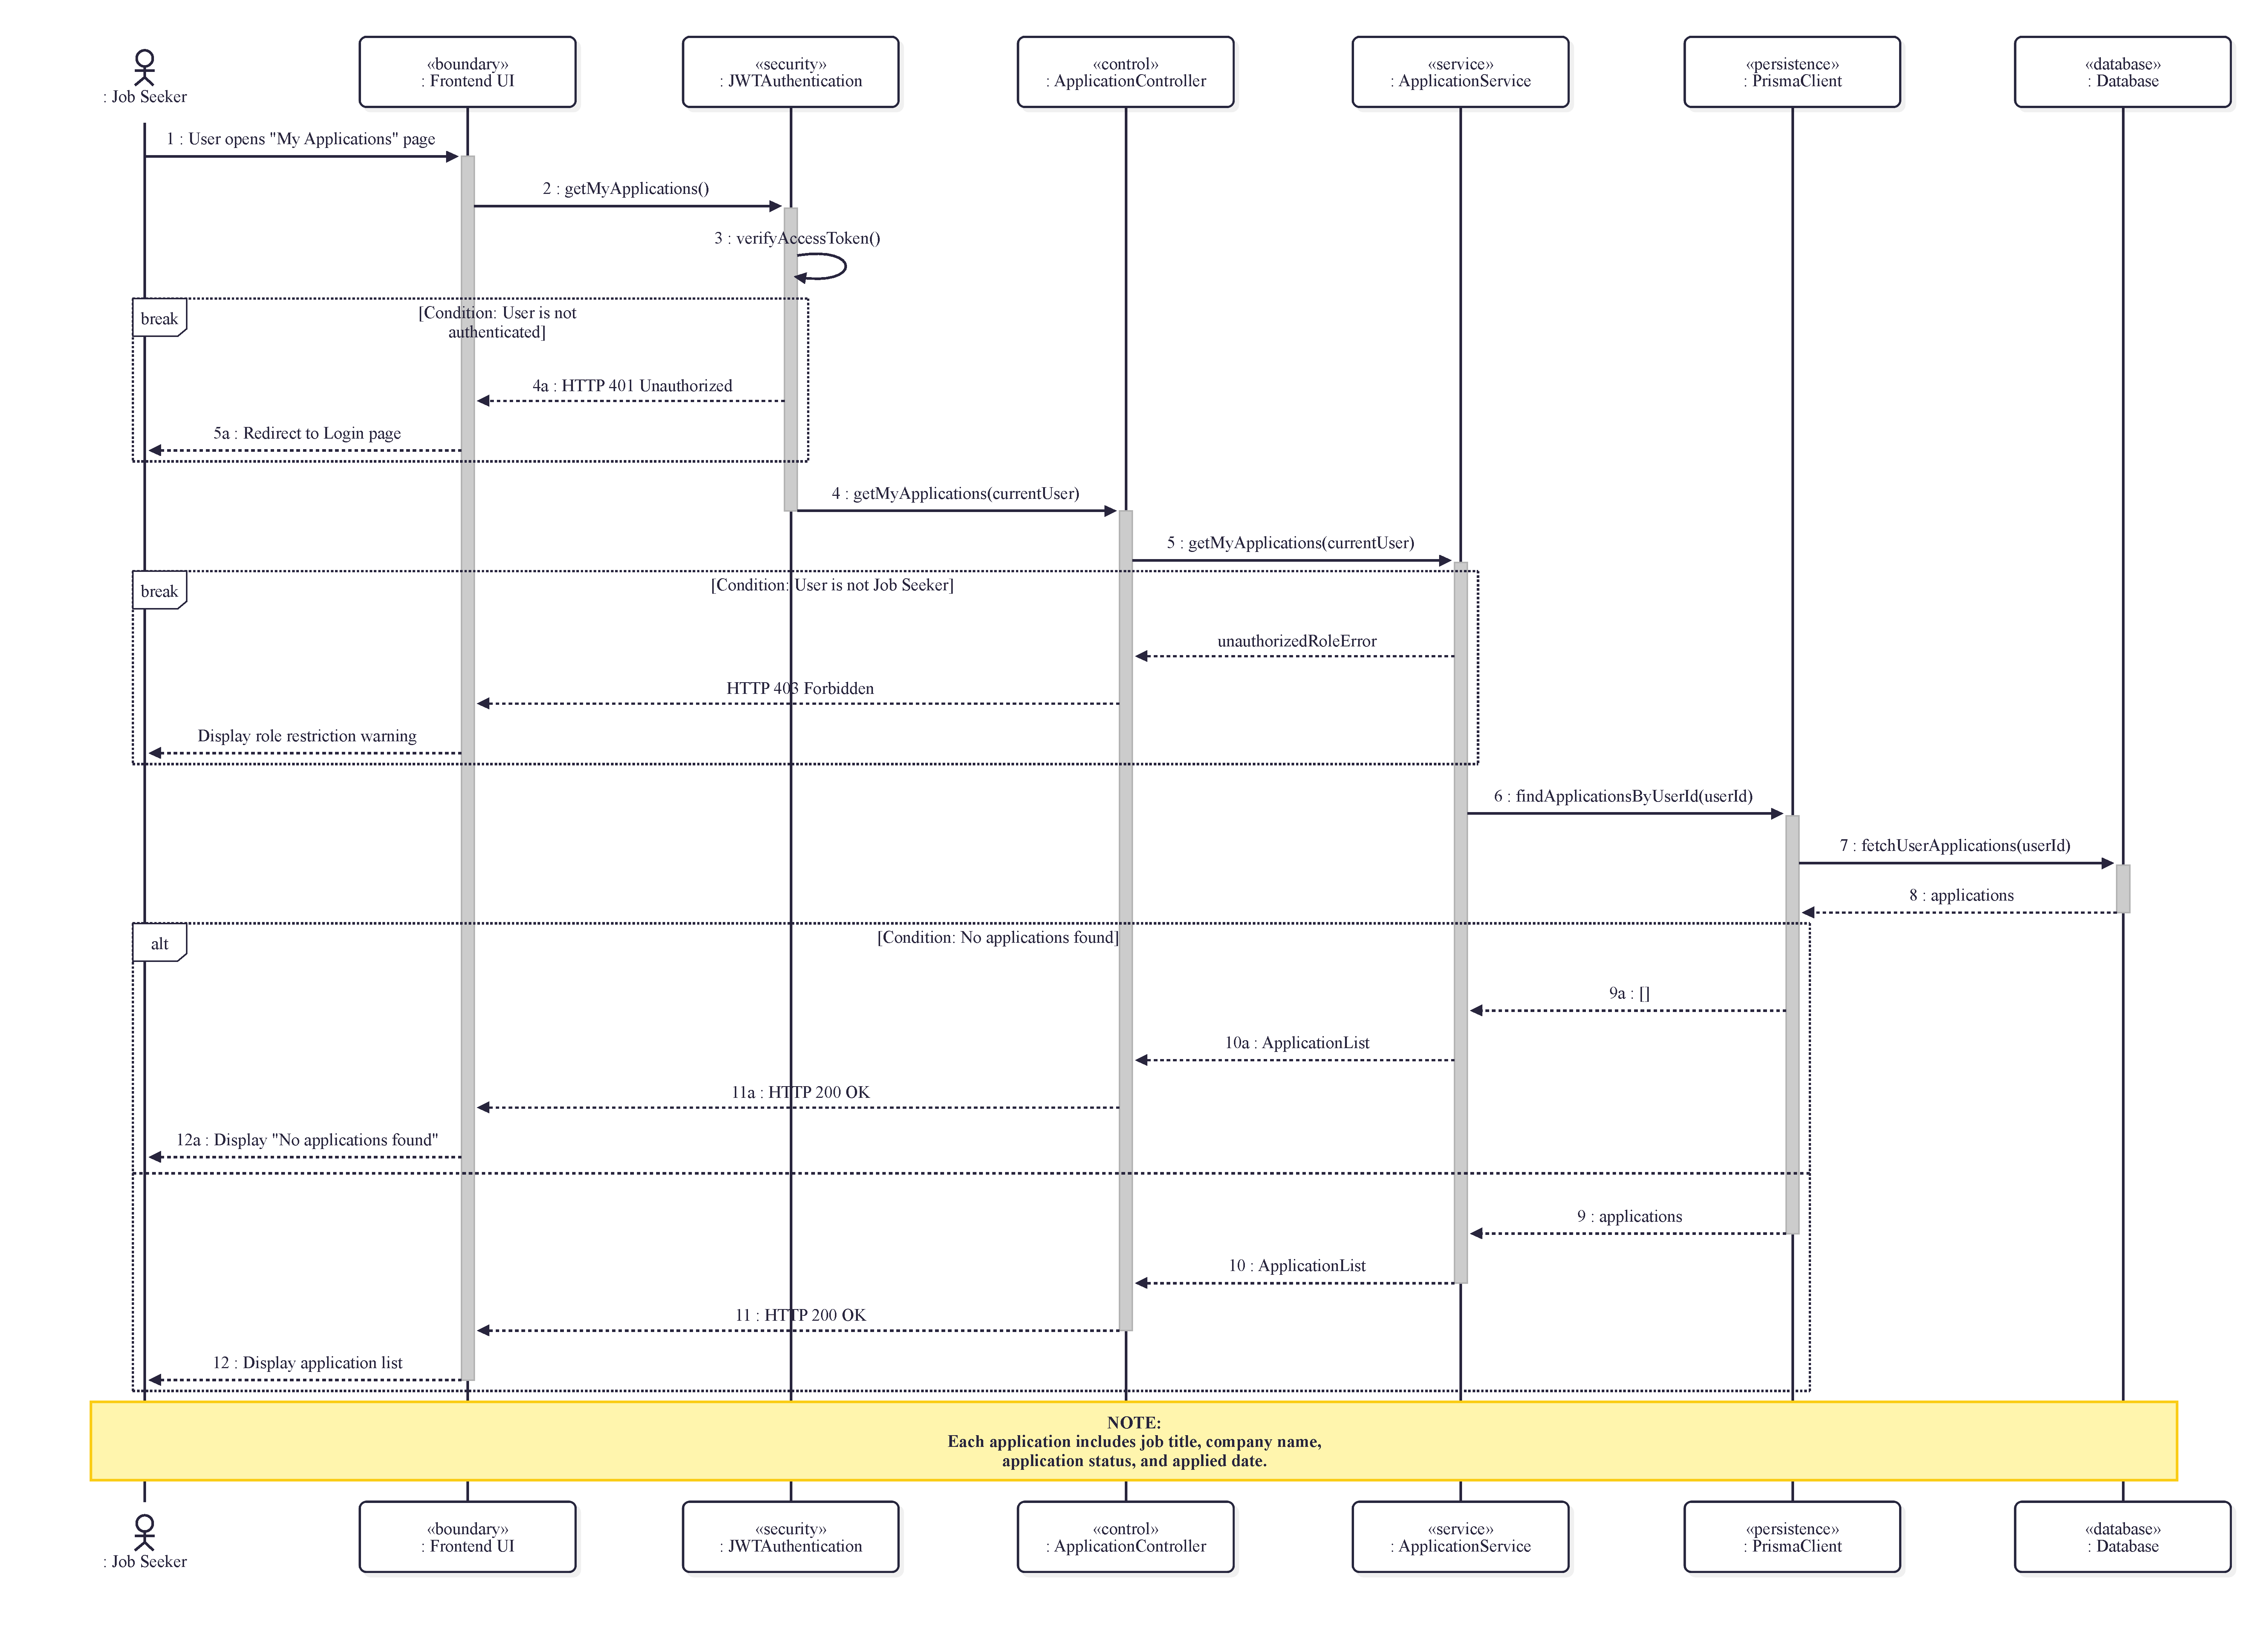
\includegraphics[width=0.9\linewidth]{diagrams/exported/5JobSeeker/SD-JobSeeker02-Track-Applications.pdf}
	\caption{Sequence Diagram: Track Applications.}
	\label{diagram:sd-jobseeker-track}
\end{figure}

\begin{figure}[H]
	\centering
	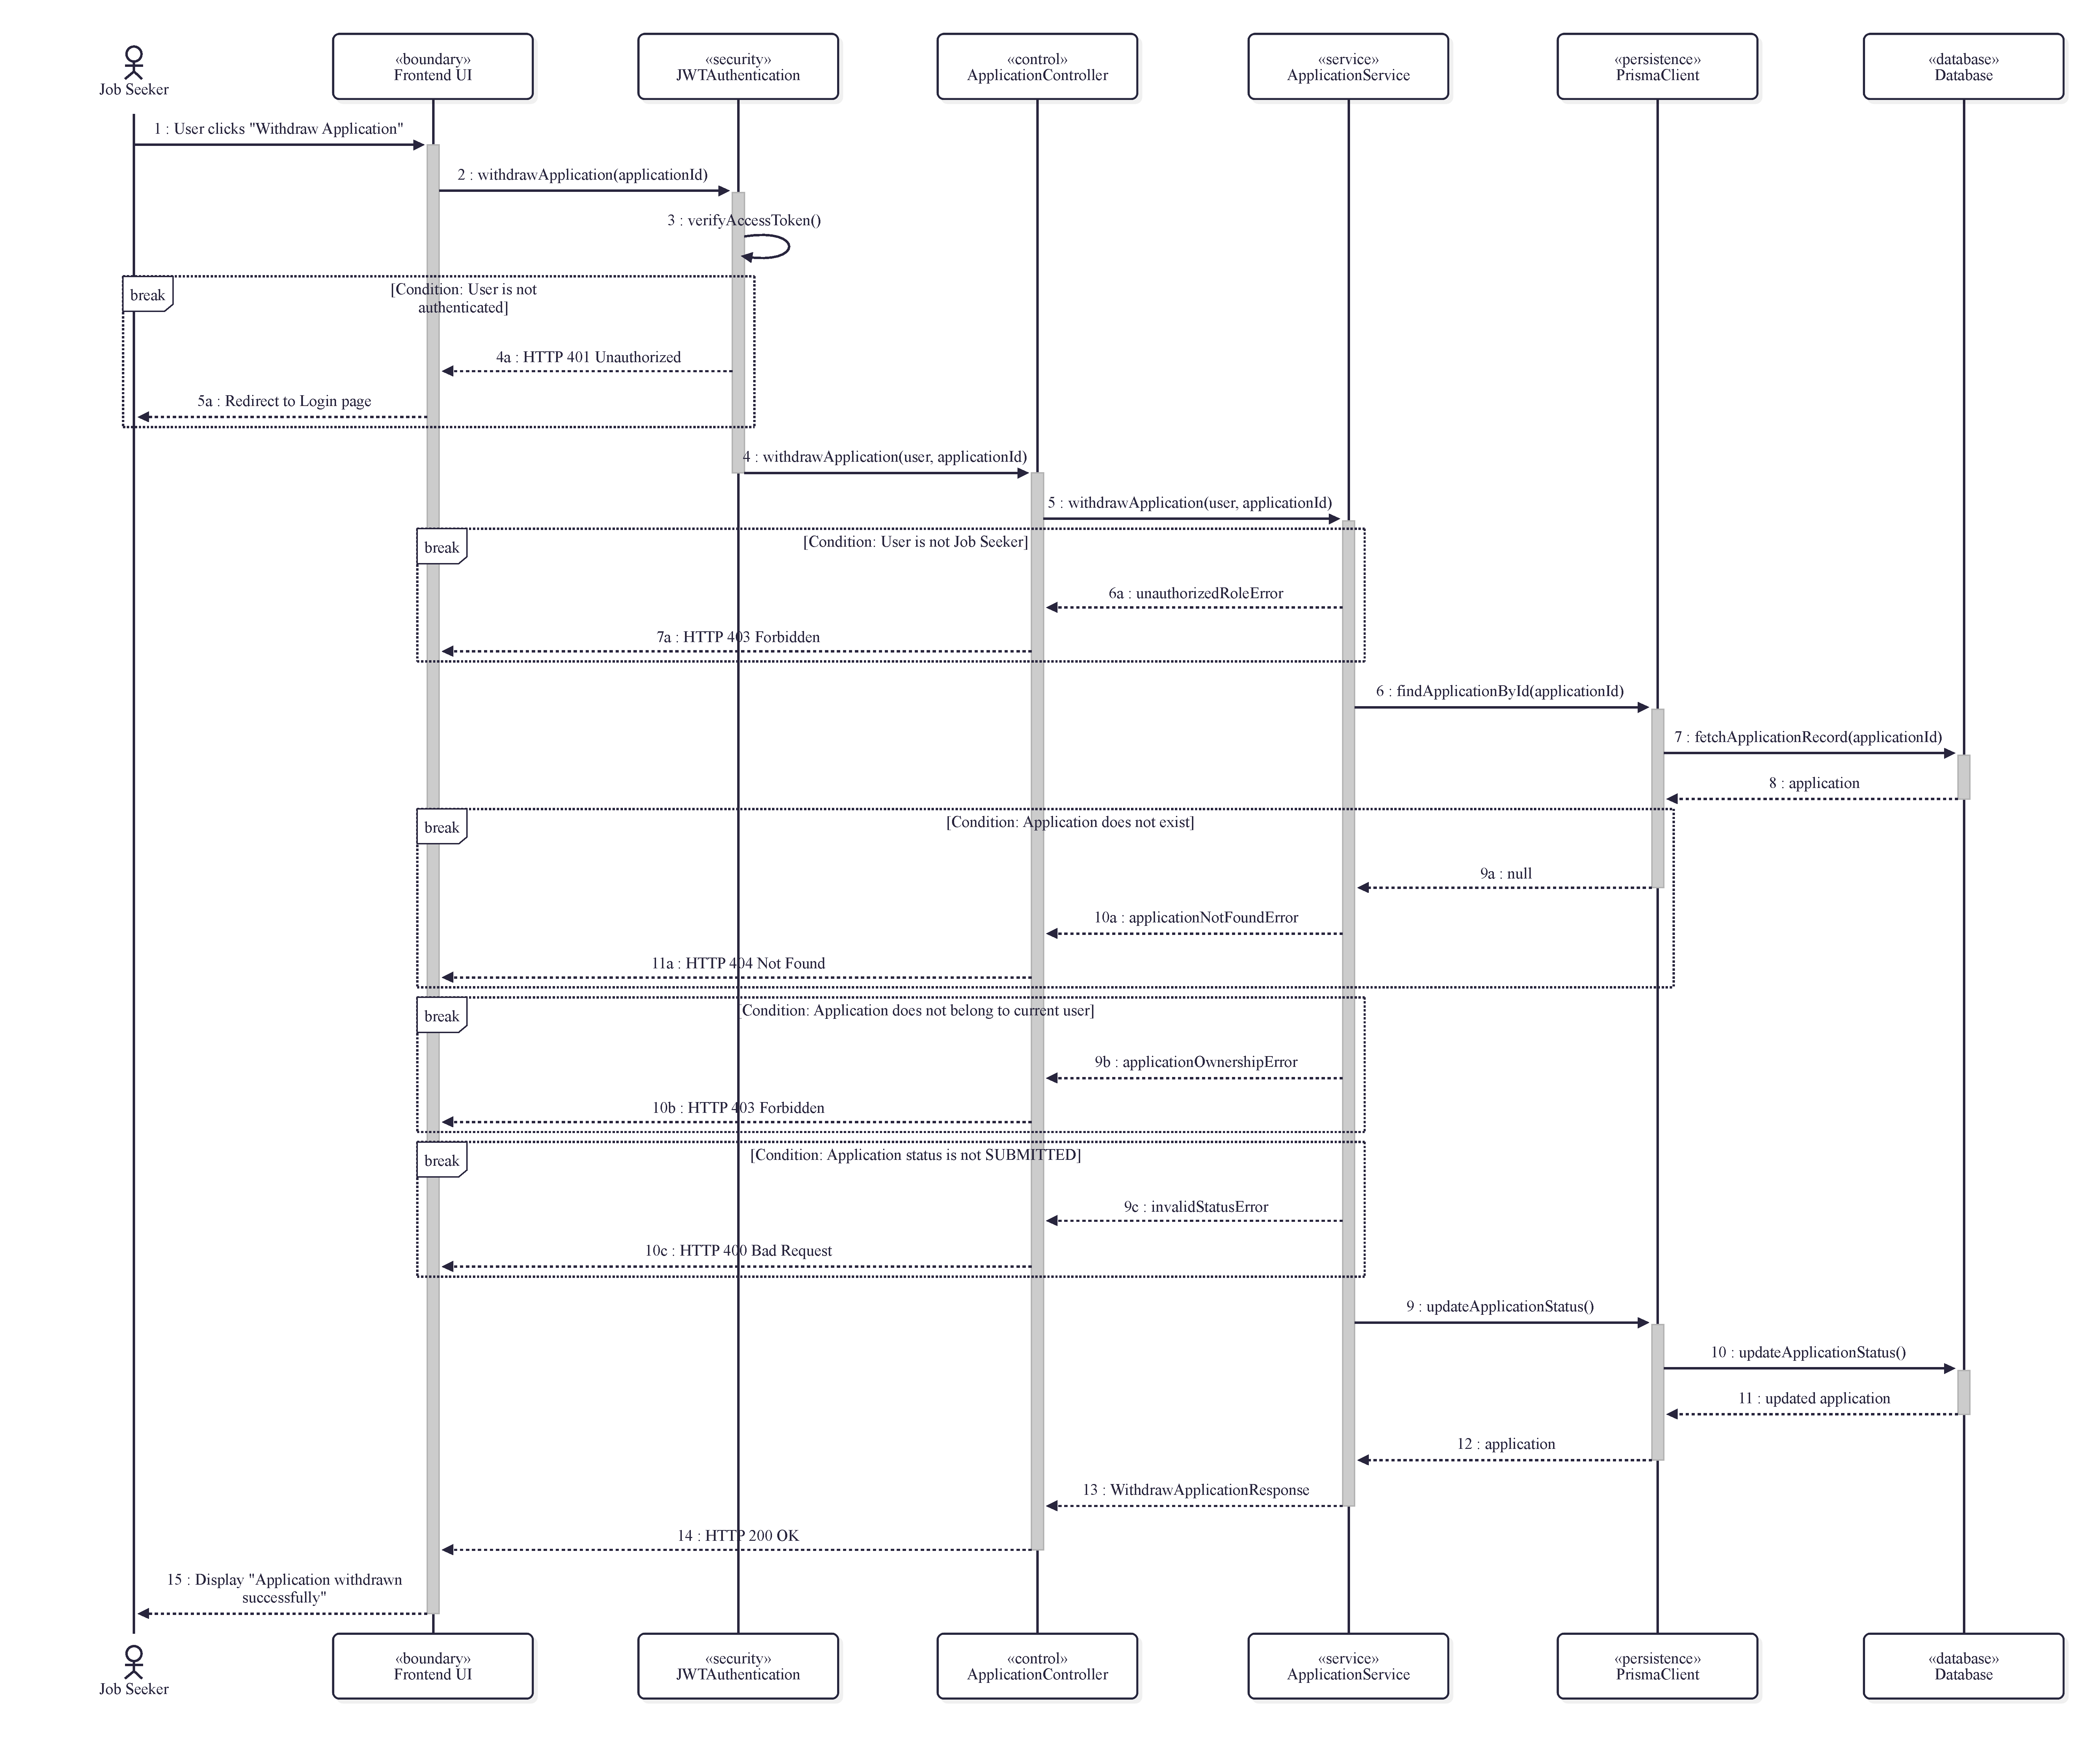
\includegraphics[width=0.9\linewidth]{diagrams/exported/5JobSeeker/SD-JobSeeker03-Cancel-Applications.pdf}
	\caption{Sequence Diagram: Cancel Applications.}
	\label{diagram:sd-jobseeker-cancel}
\end{figure}

\section{Employer Job Management}

\begin{figure}[H]
	\centering
	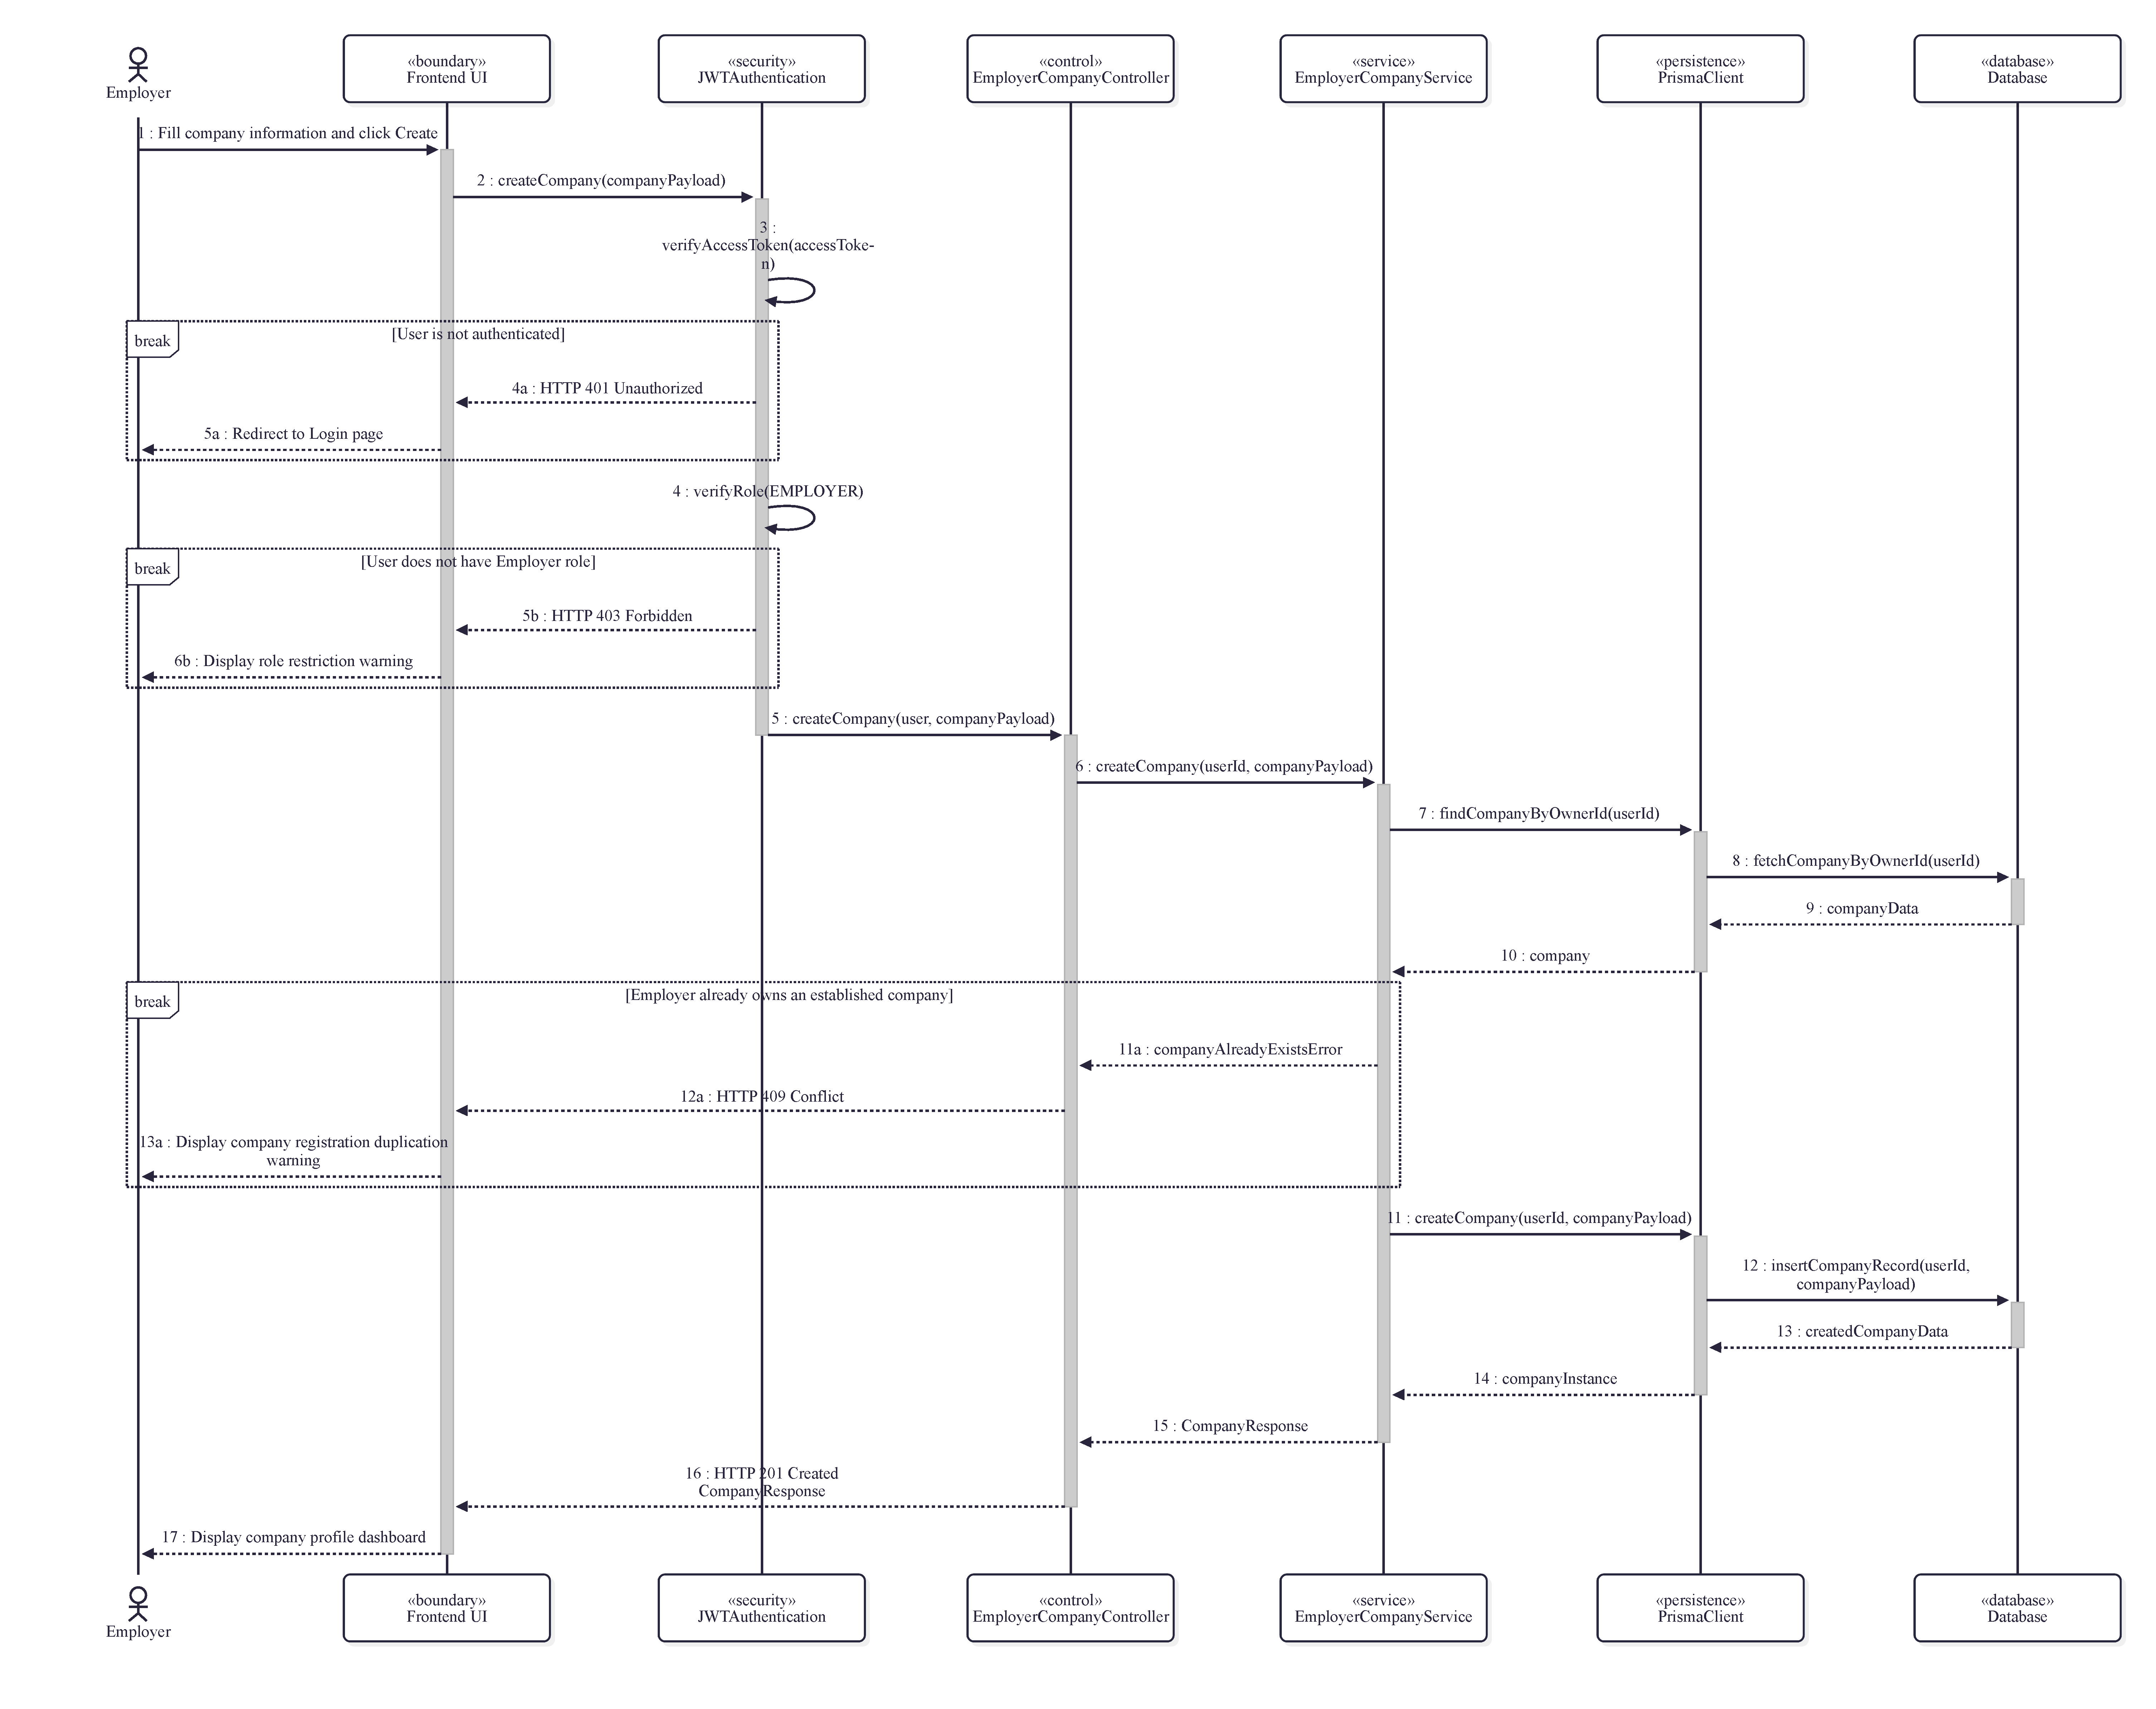
\includegraphics[width=0.9\linewidth]{diagrams/exported/6Employer/SD-Employer00-Create-Company-Profile.pdf}
	\caption{Sequence Diagram: Create Company Profile.}
	\label{diagram:sd-employer-company}
\end{figure}

\begin{figure}[H]
	\centering
	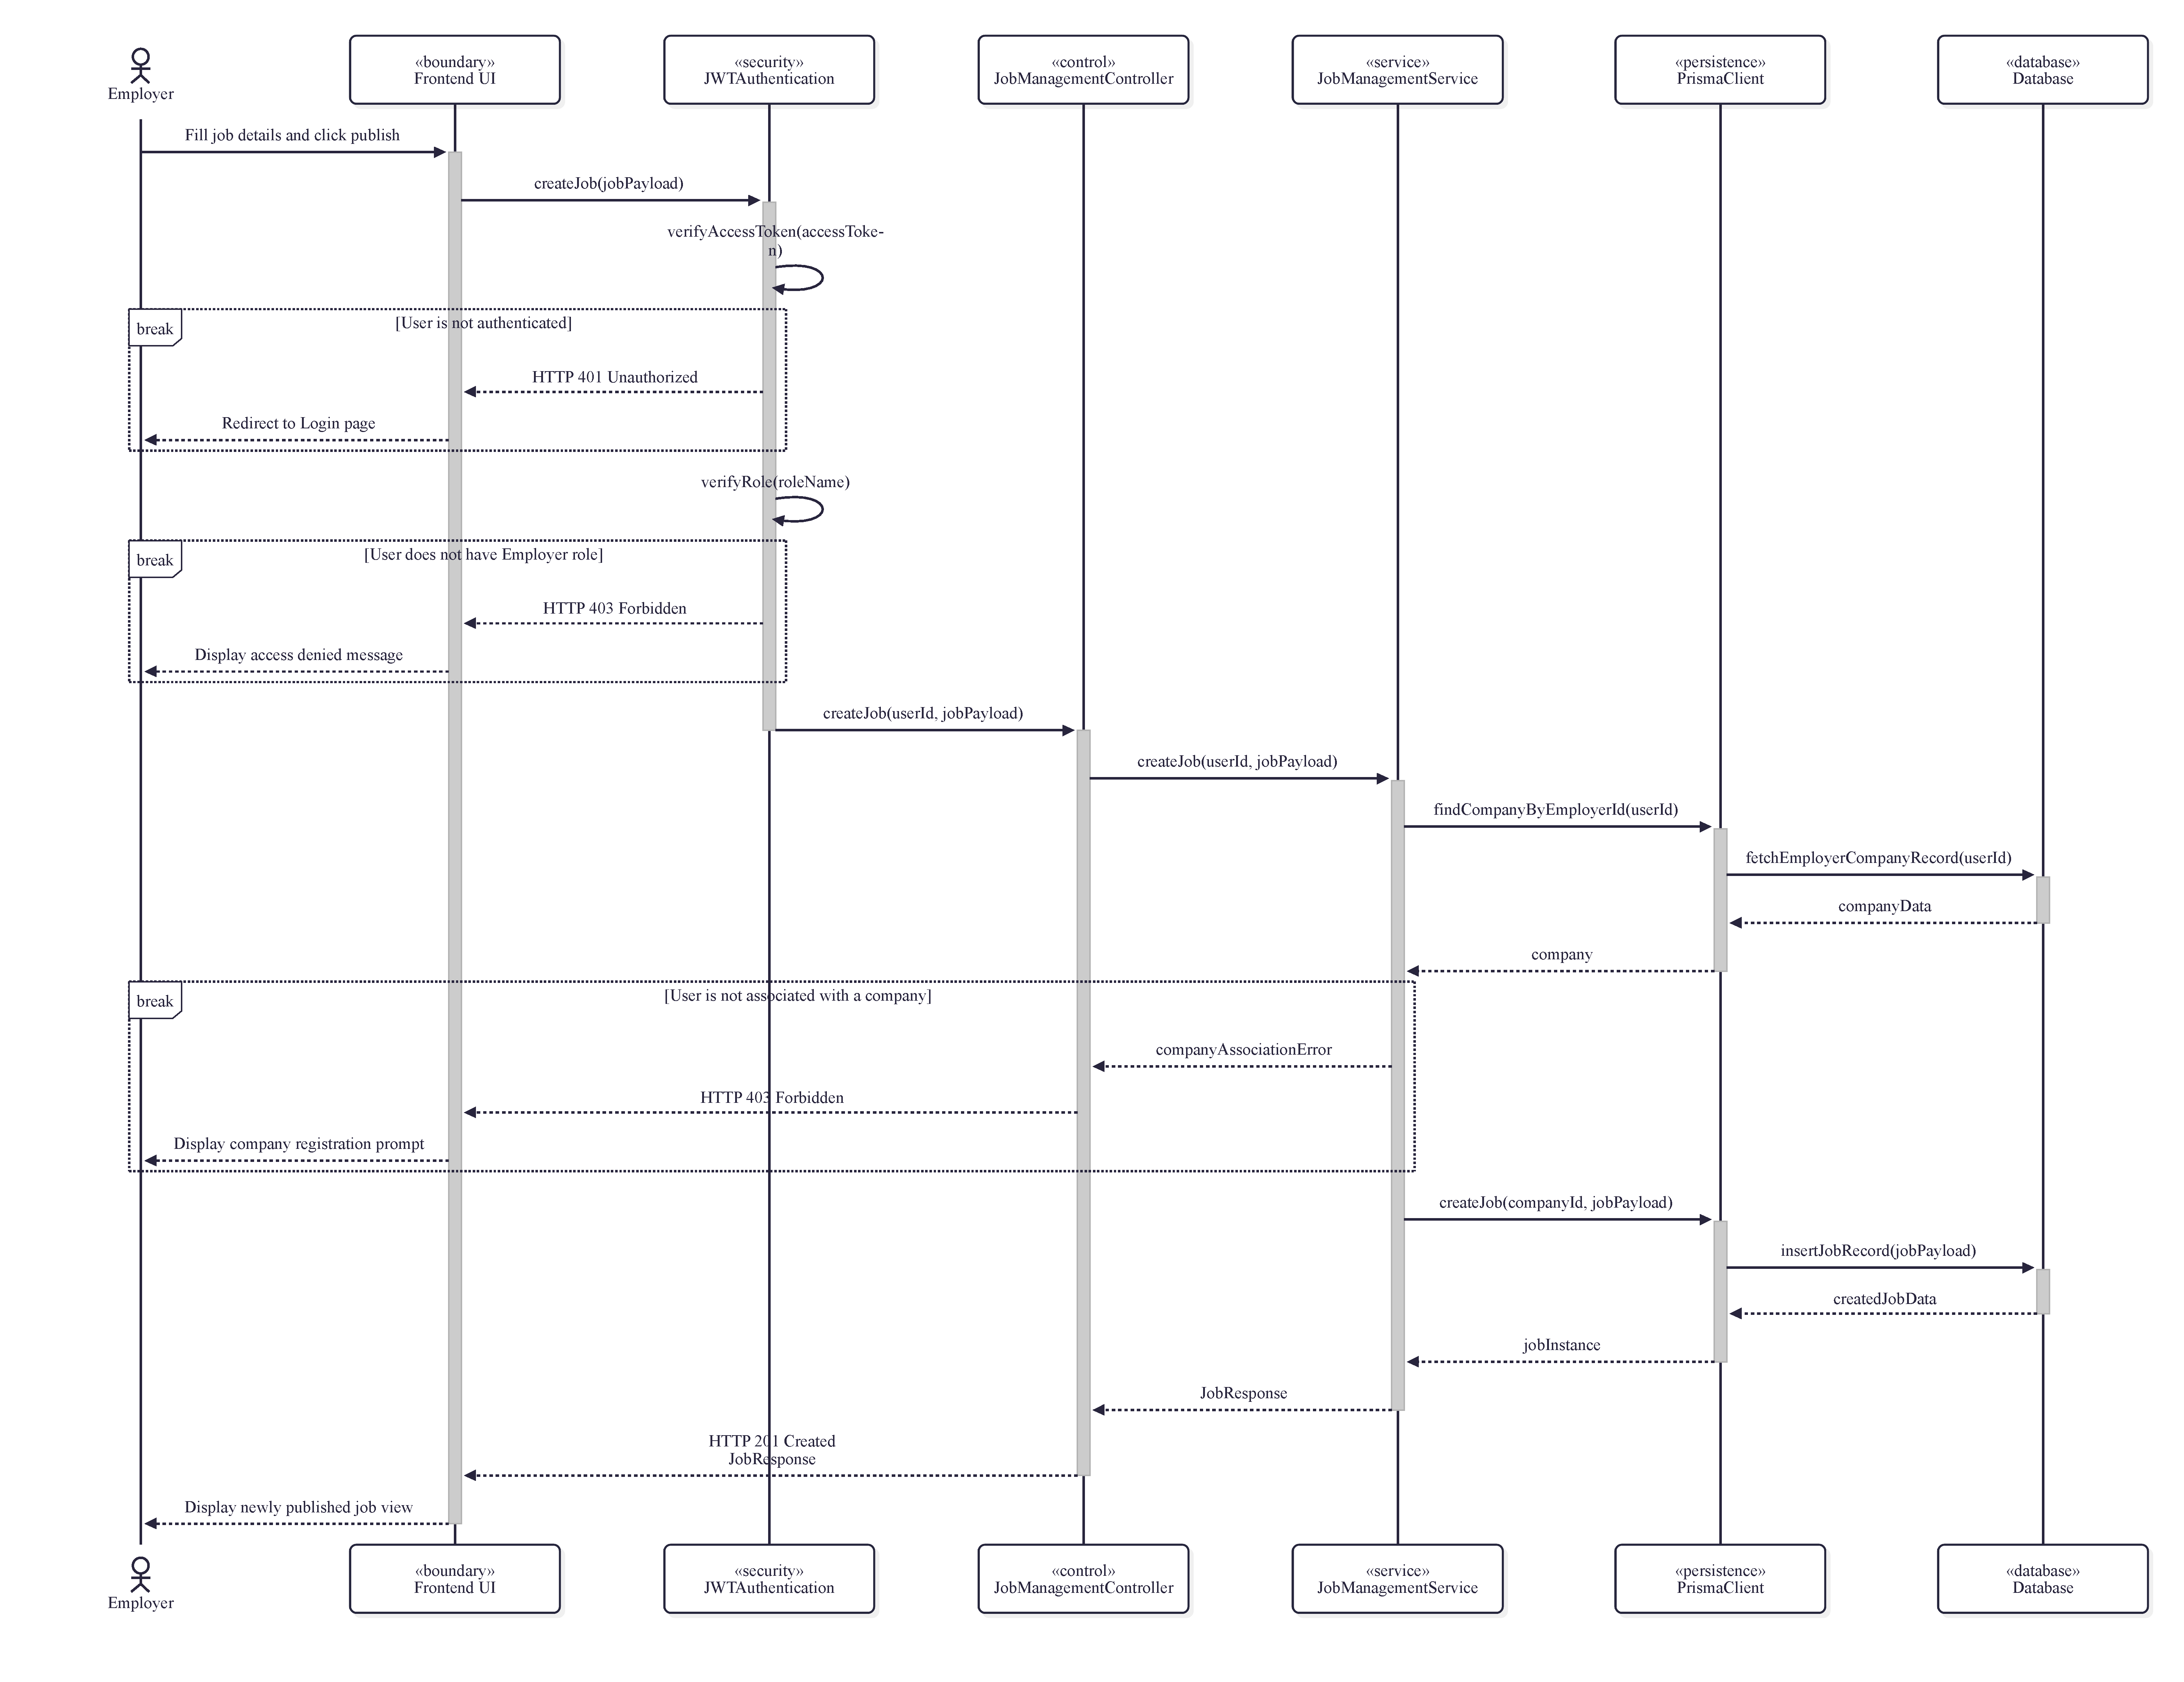
\includegraphics[width=0.9\linewidth]{diagrams/exported/6Employer/SD-Employer01-Create-Job-Posting.pdf}
	\caption{Sequence Diagram: Create Job Posting.}
	\label{diagram:sd-employer-create-job}
\end{figure}

\begin{figure}[H]
	\centering
	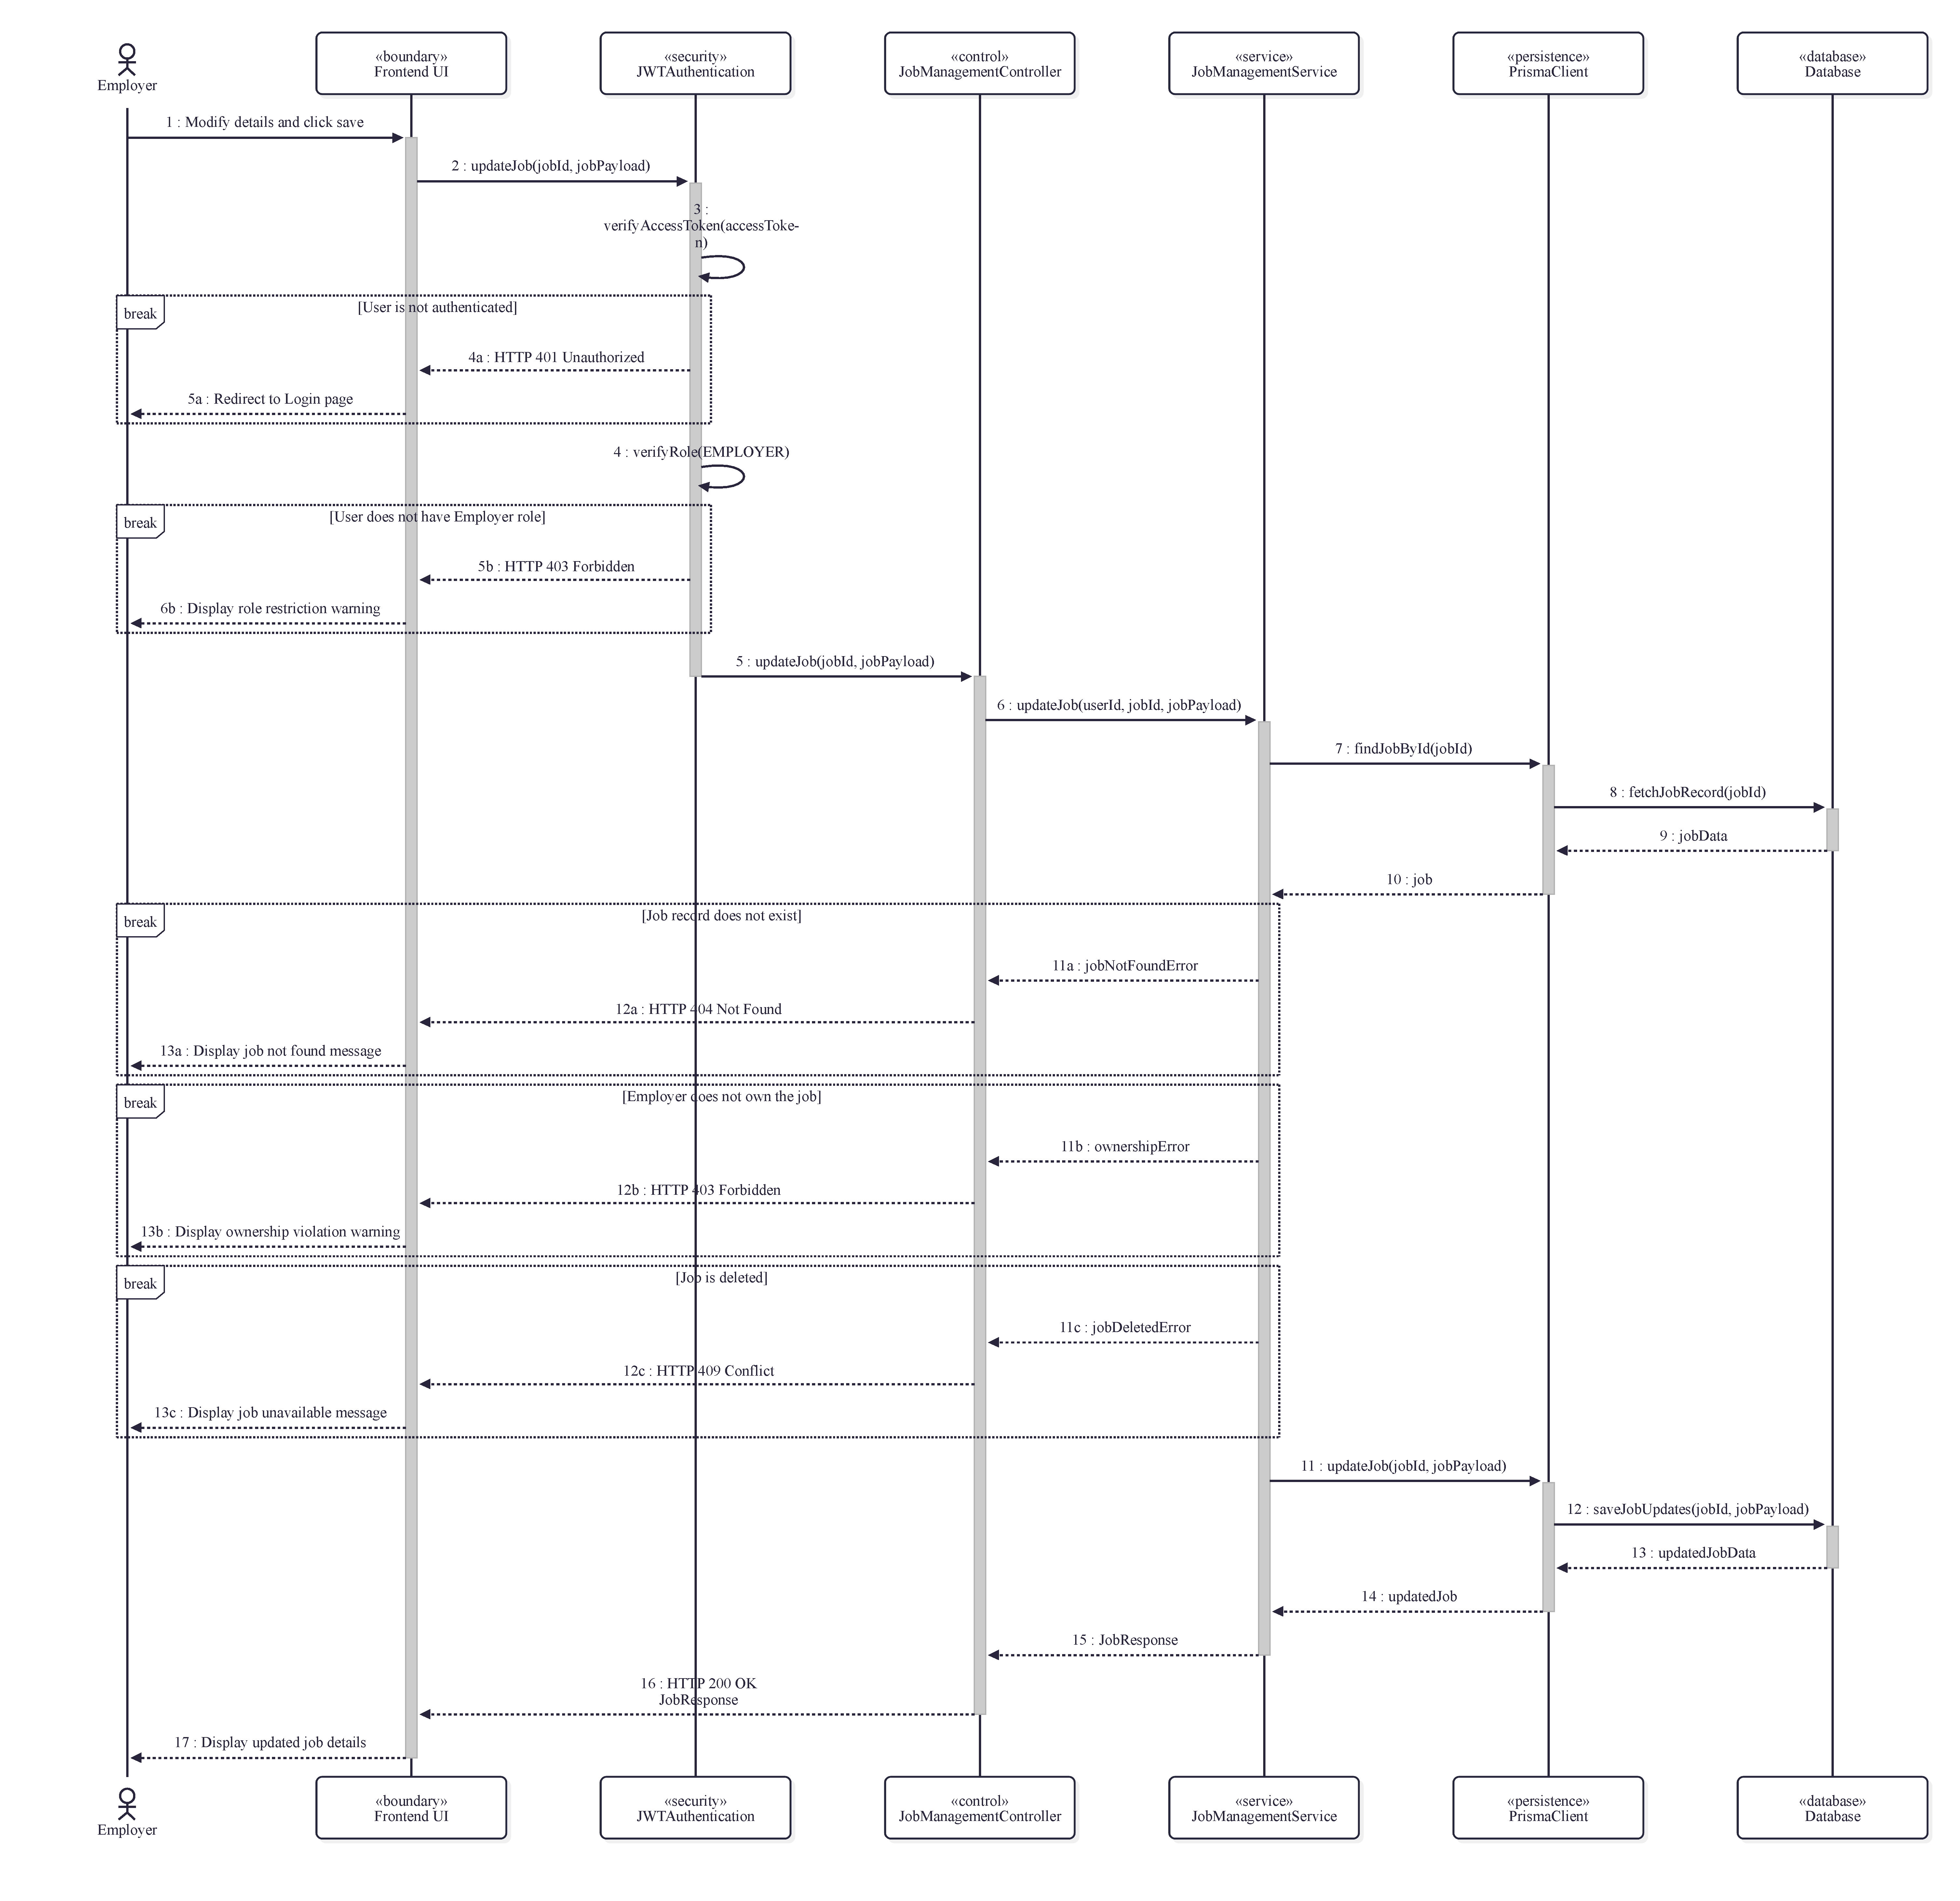
\includegraphics[width=0.9\linewidth]{diagrams/exported/6Employer/SD-Employer02-Edit-Job-Posting.pdf}
	\caption{Sequence Diagram: Edit Job Posting.}
	\label{diagram:sd-employer-edit-job}
\end{figure}

\begin{figure}[H]
	\centering
	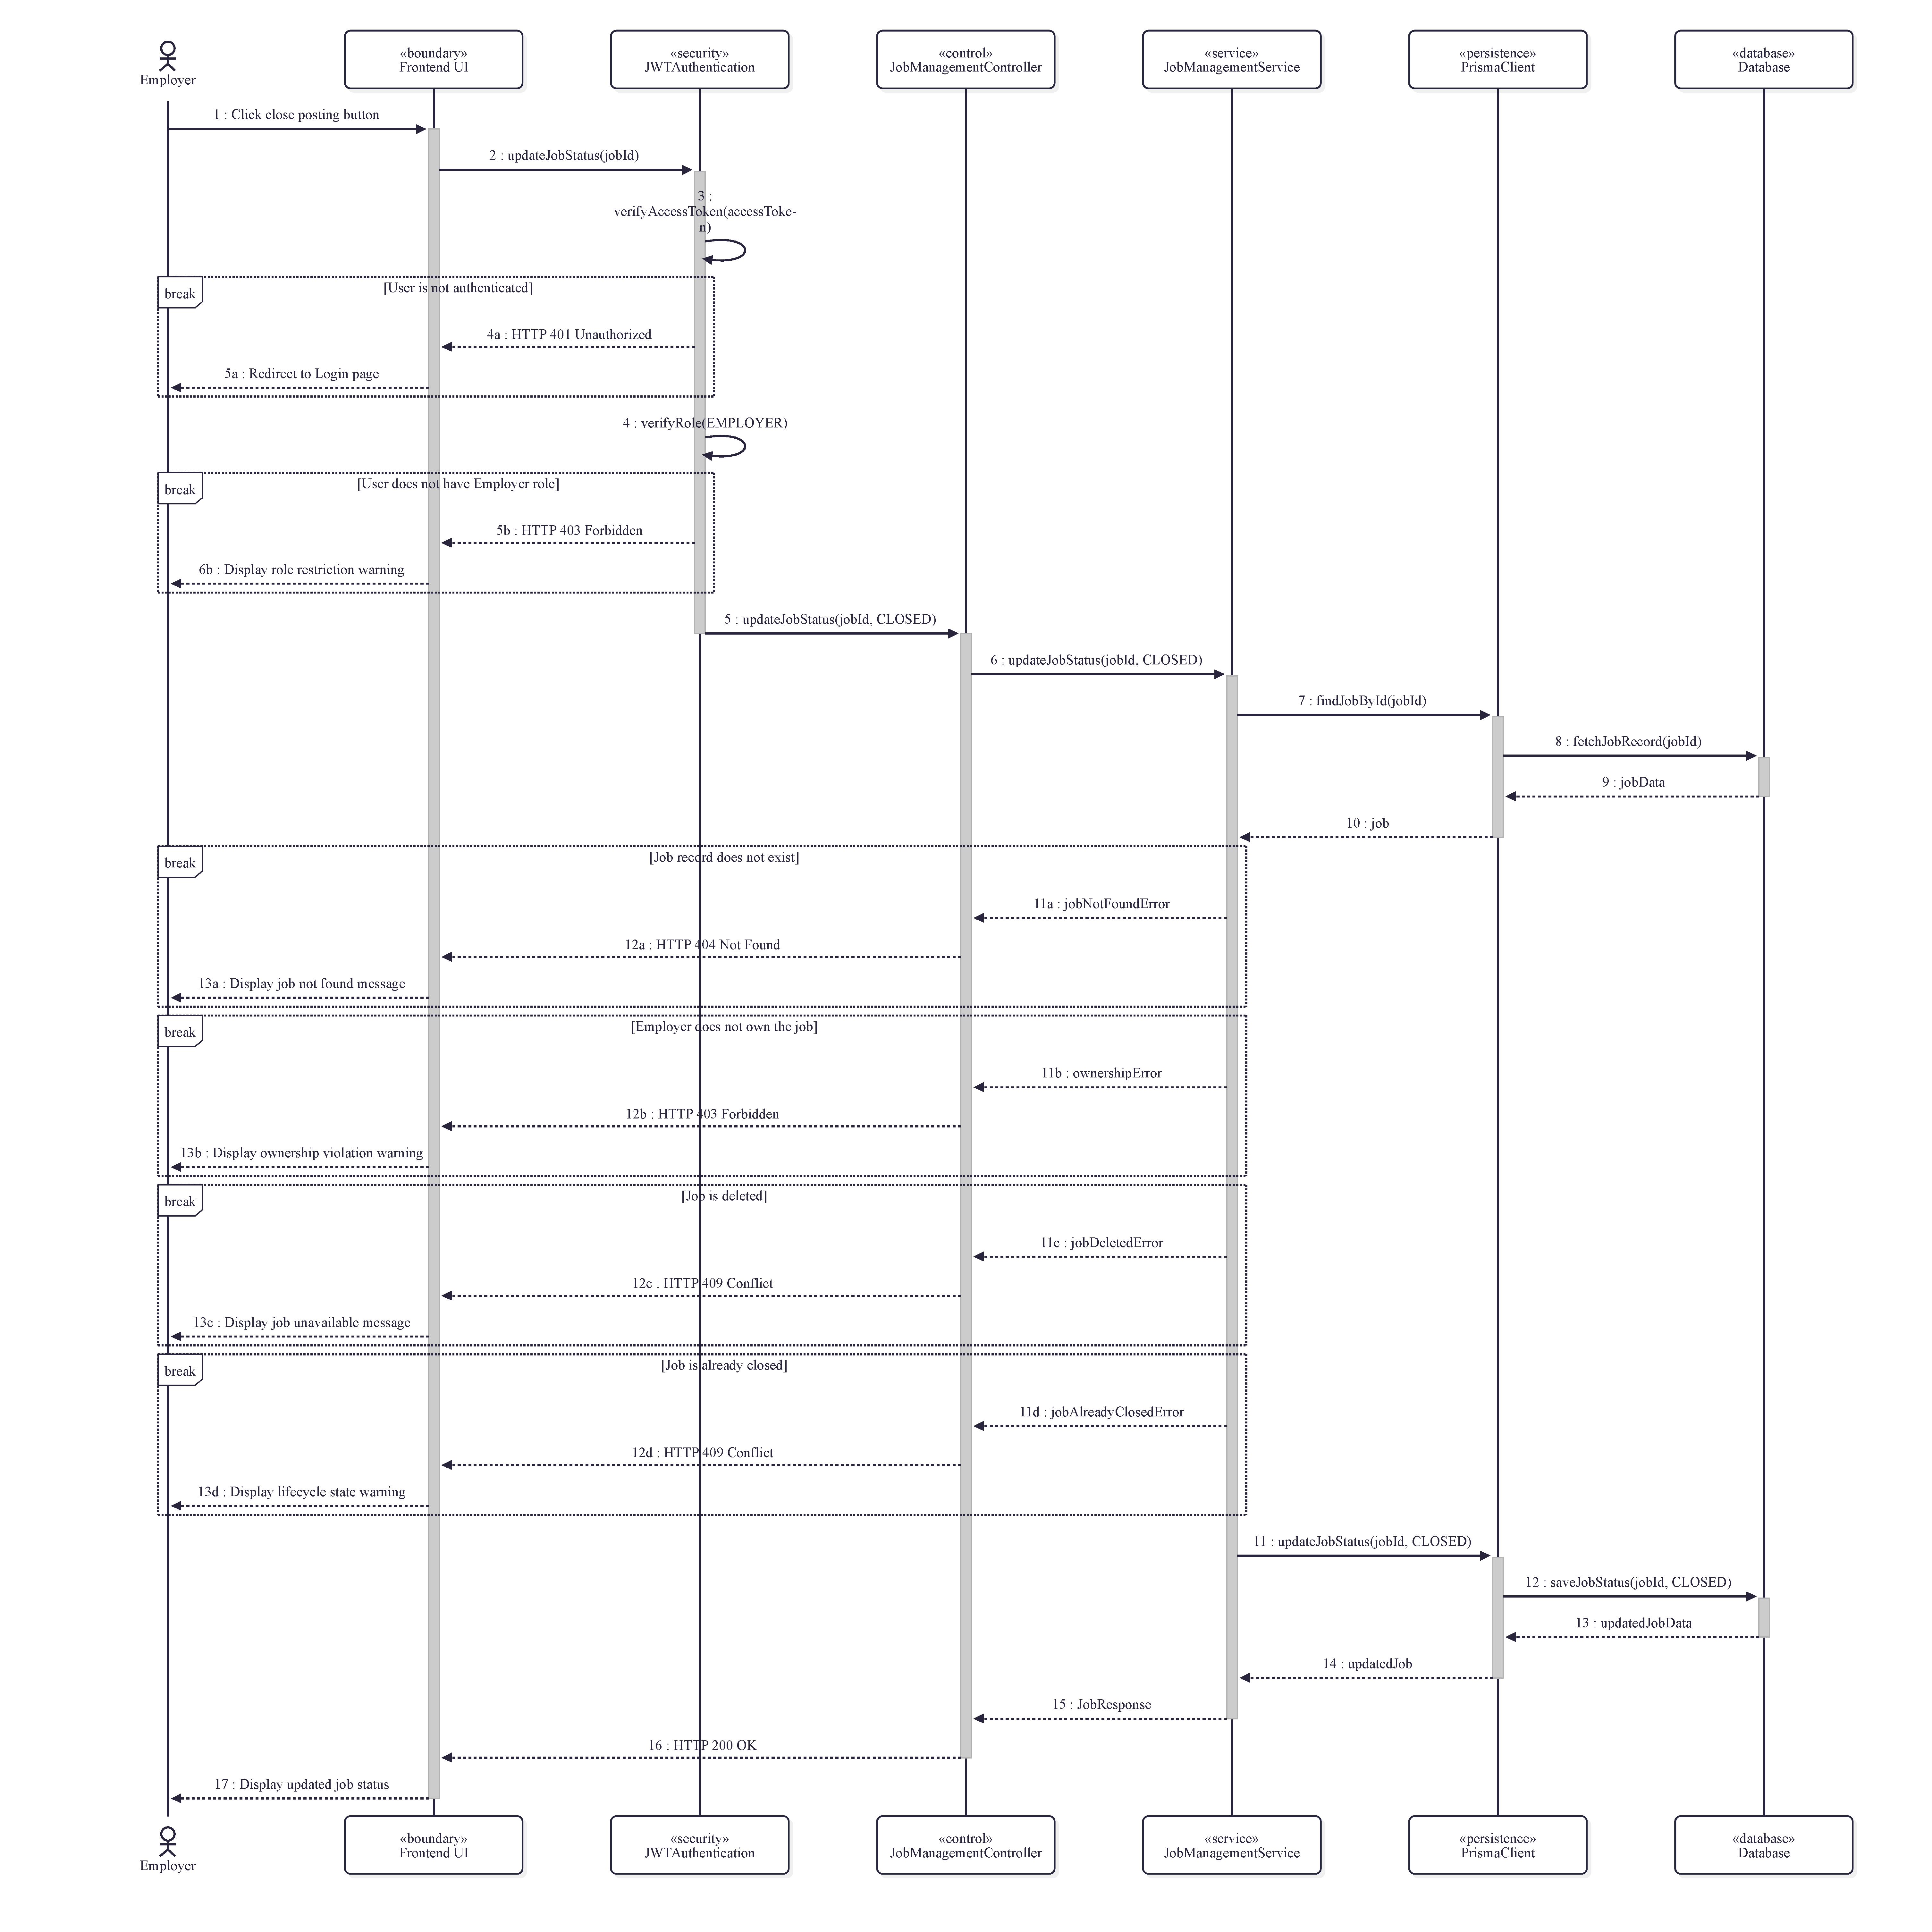
\includegraphics[width=0.9\linewidth]{diagrams/exported/6Employer/SD-Employer03-Close-Job-Posting.pdf}
	\caption{Sequence Diagram: Close Job Posting.}
	\label{diagram:sd-employer-close-job}
\end{figure}

\begin{figure}[H]
	\centering
	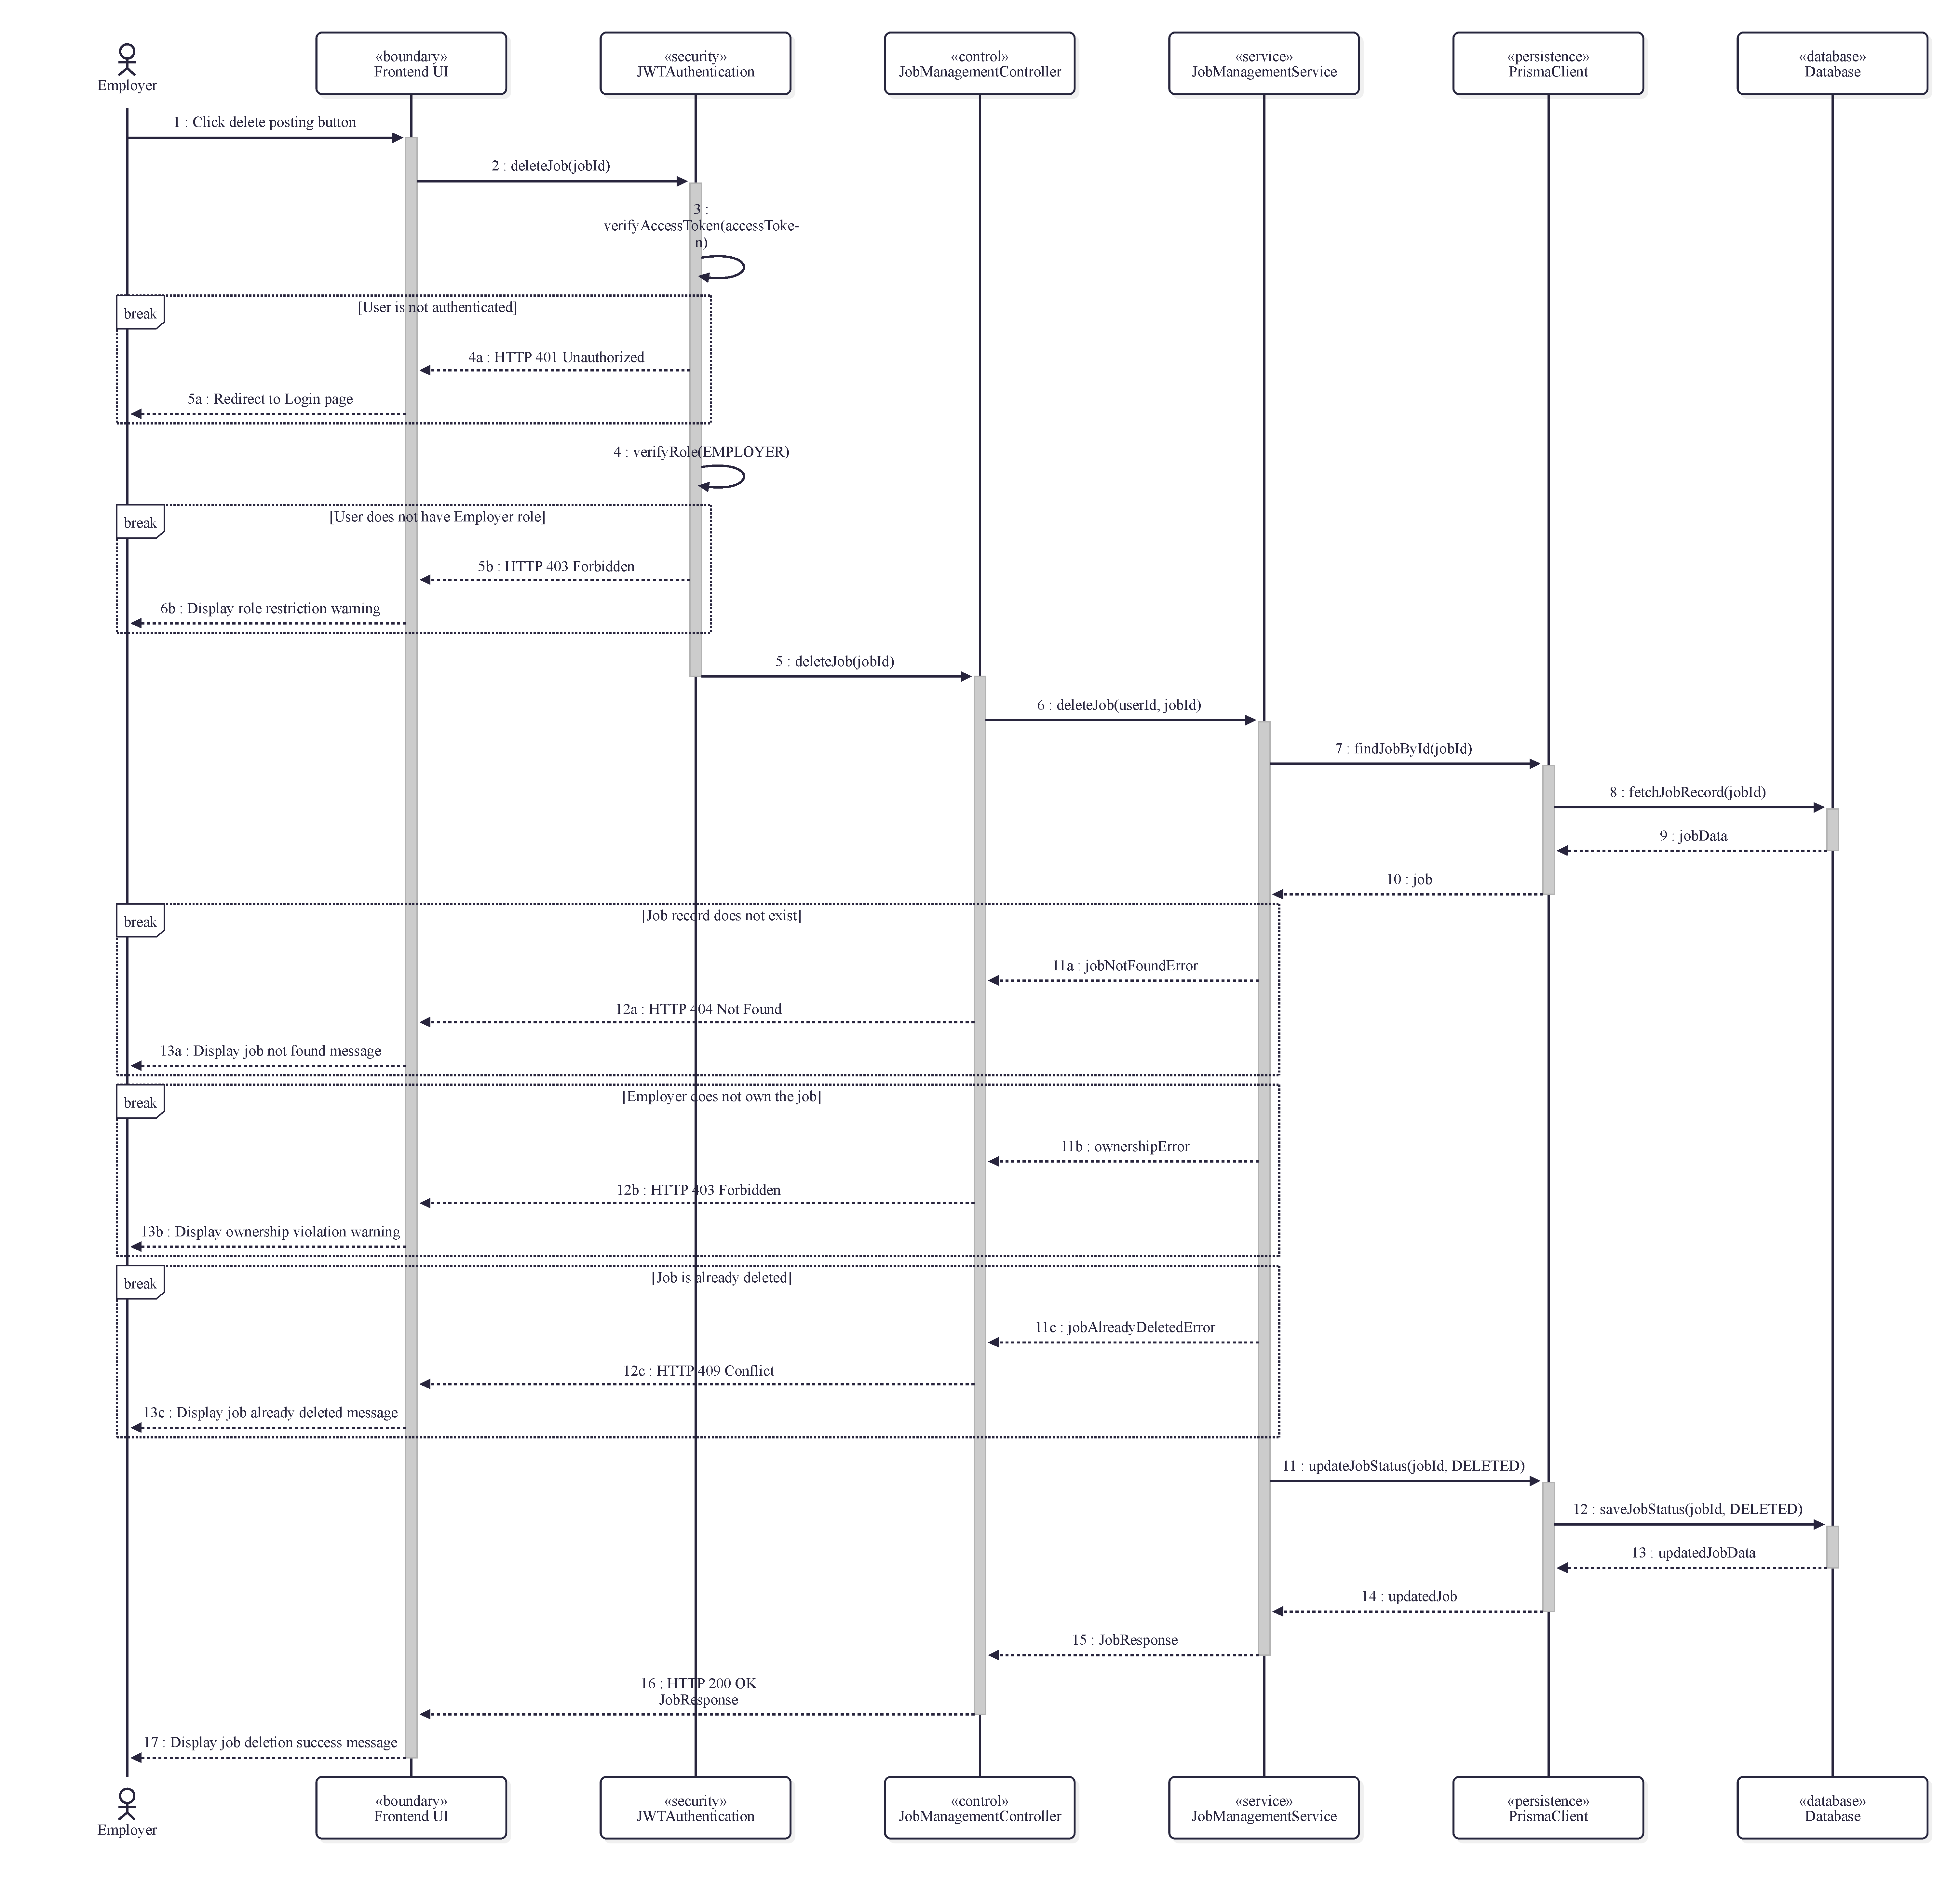
\includegraphics[width=0.9\linewidth]{diagrams/exported/6Employer/SD-Employer04-Delete-Job-Posting.pdf}
	\caption{Sequence Diagram: Delete Job Posting.}
	\label{diagram:sd-employer-delete-job}
\end{figure}

\begin{figure}[H]
	\centering
	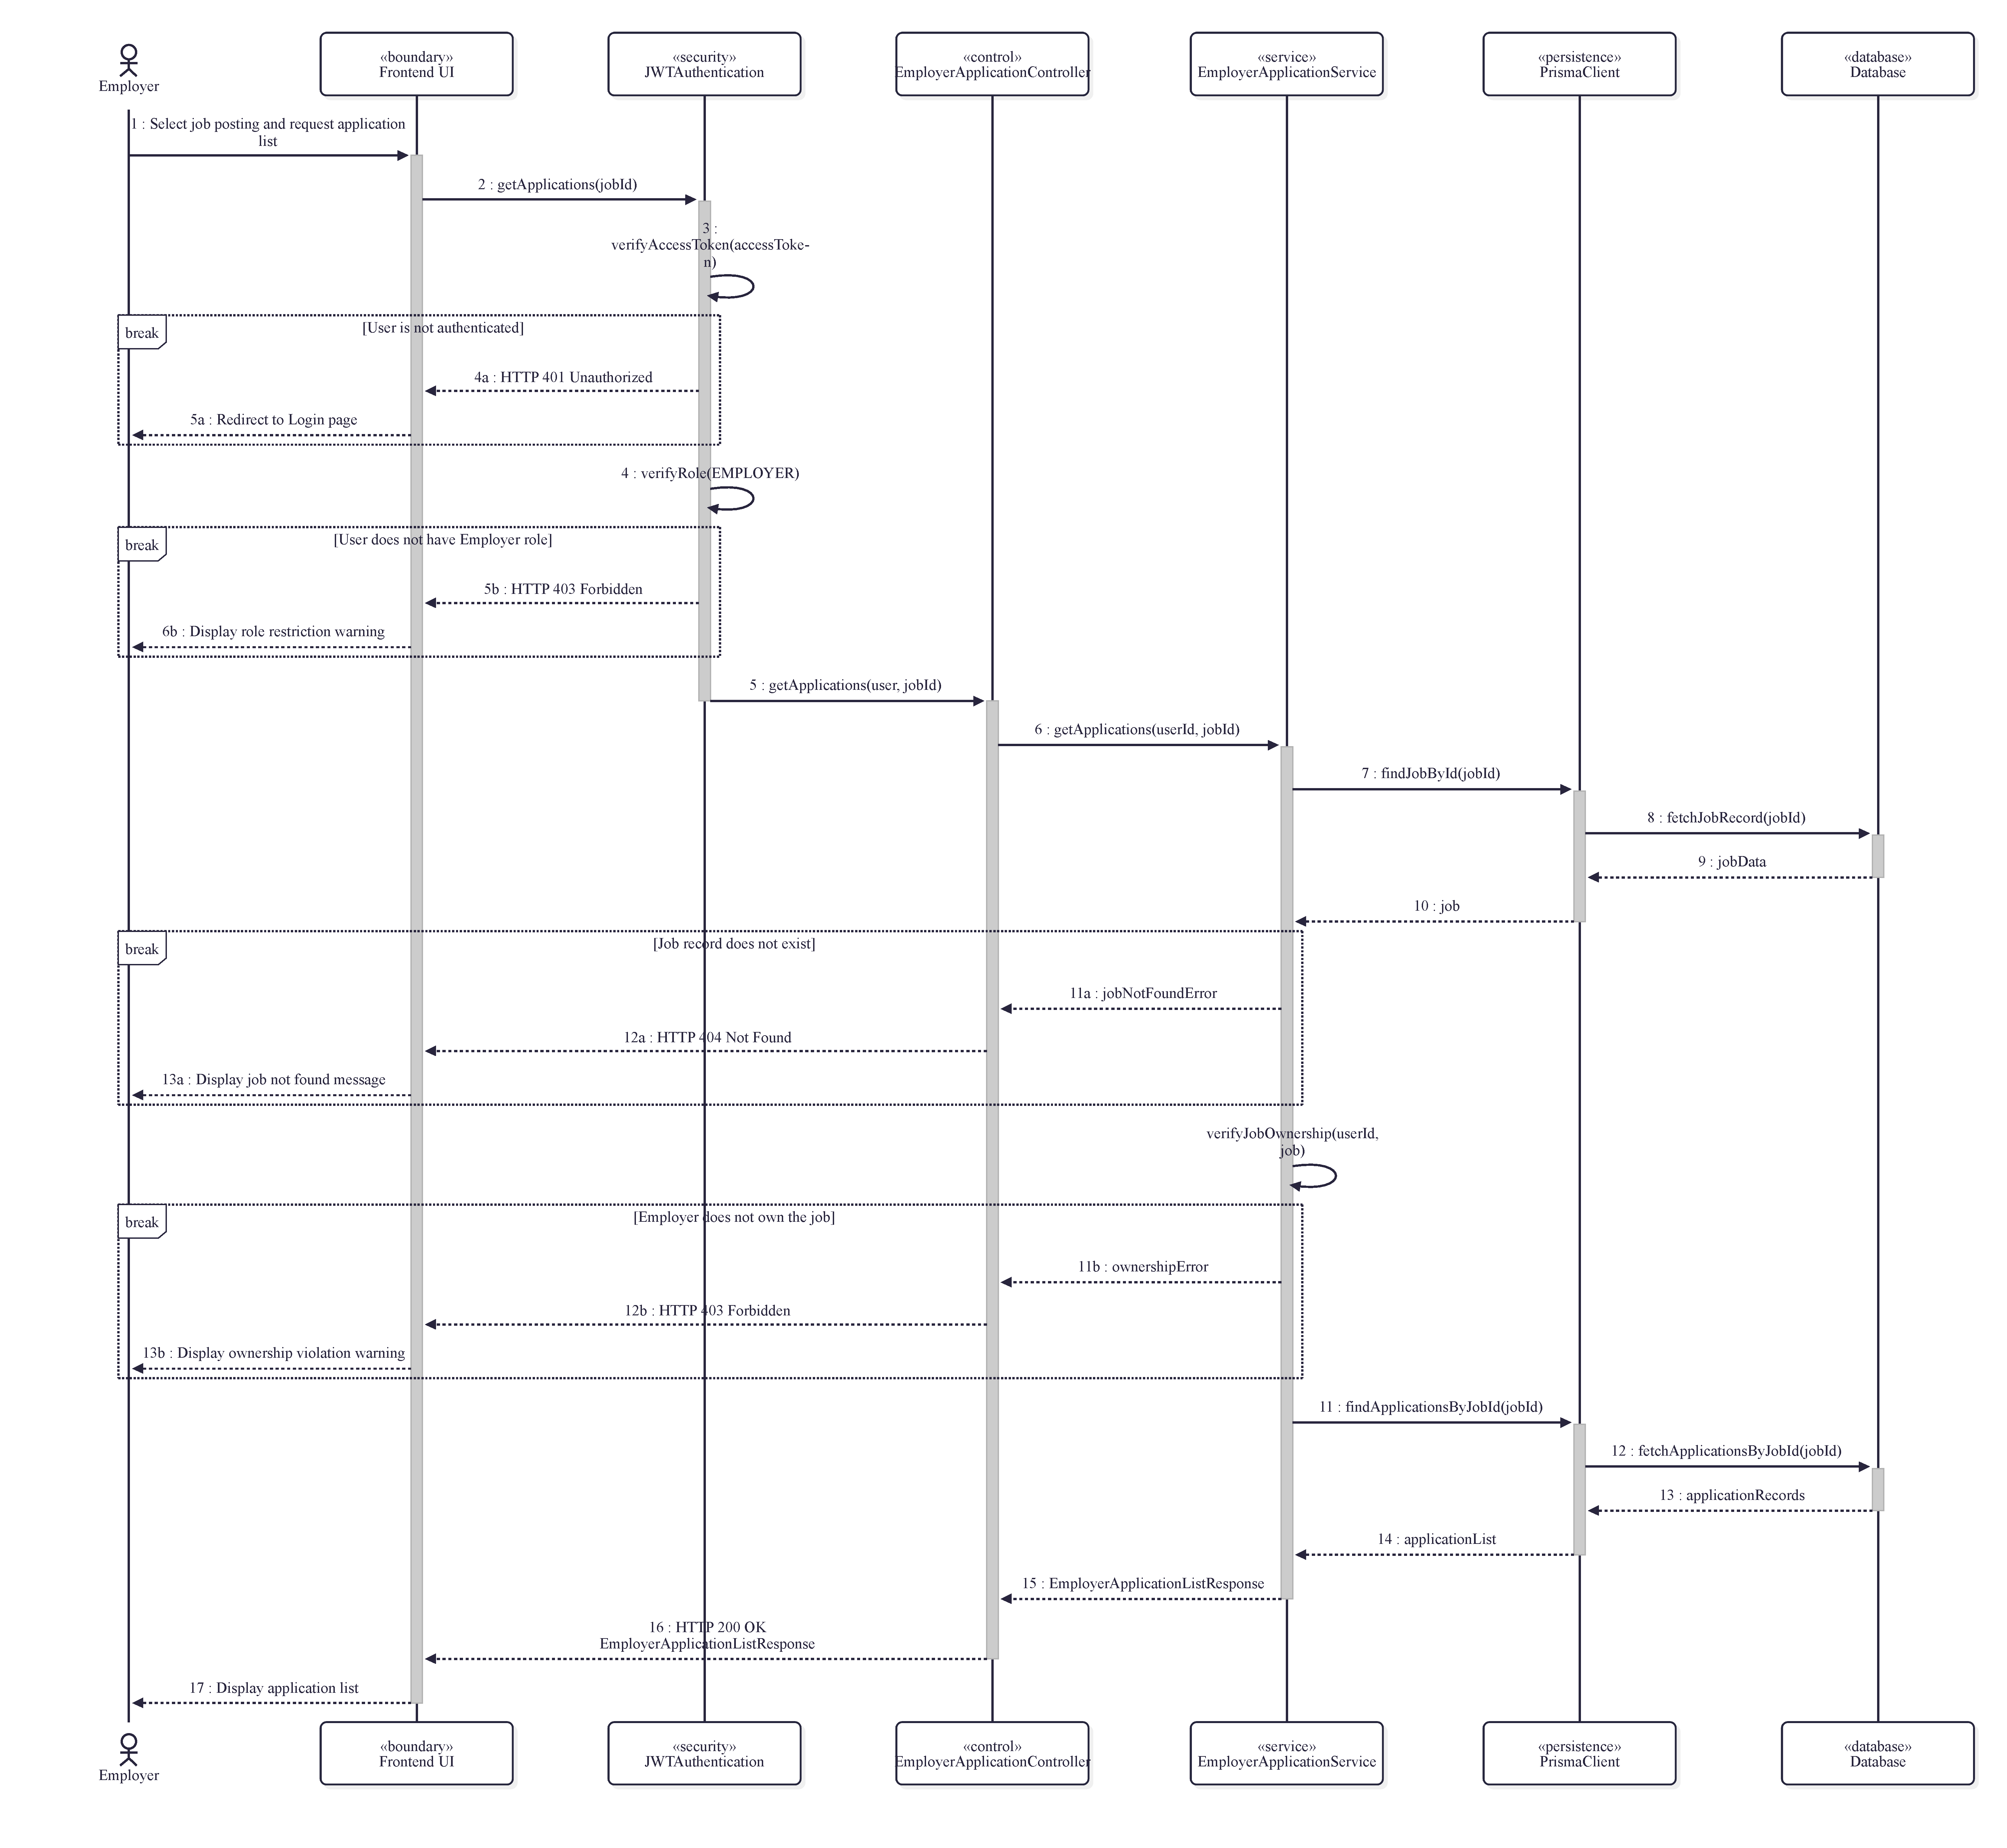
\includegraphics[width=0.9\linewidth]{diagrams/exported/6Employer/SD-Employer05-Review-Application.pdf}
	\caption{Sequence Diagram: Review Application.}
	\label{diagram:sd-employer-review-application}
\end{figure}

\section{Authentication and Profile}

\begin{figure}[H]
	\centering
	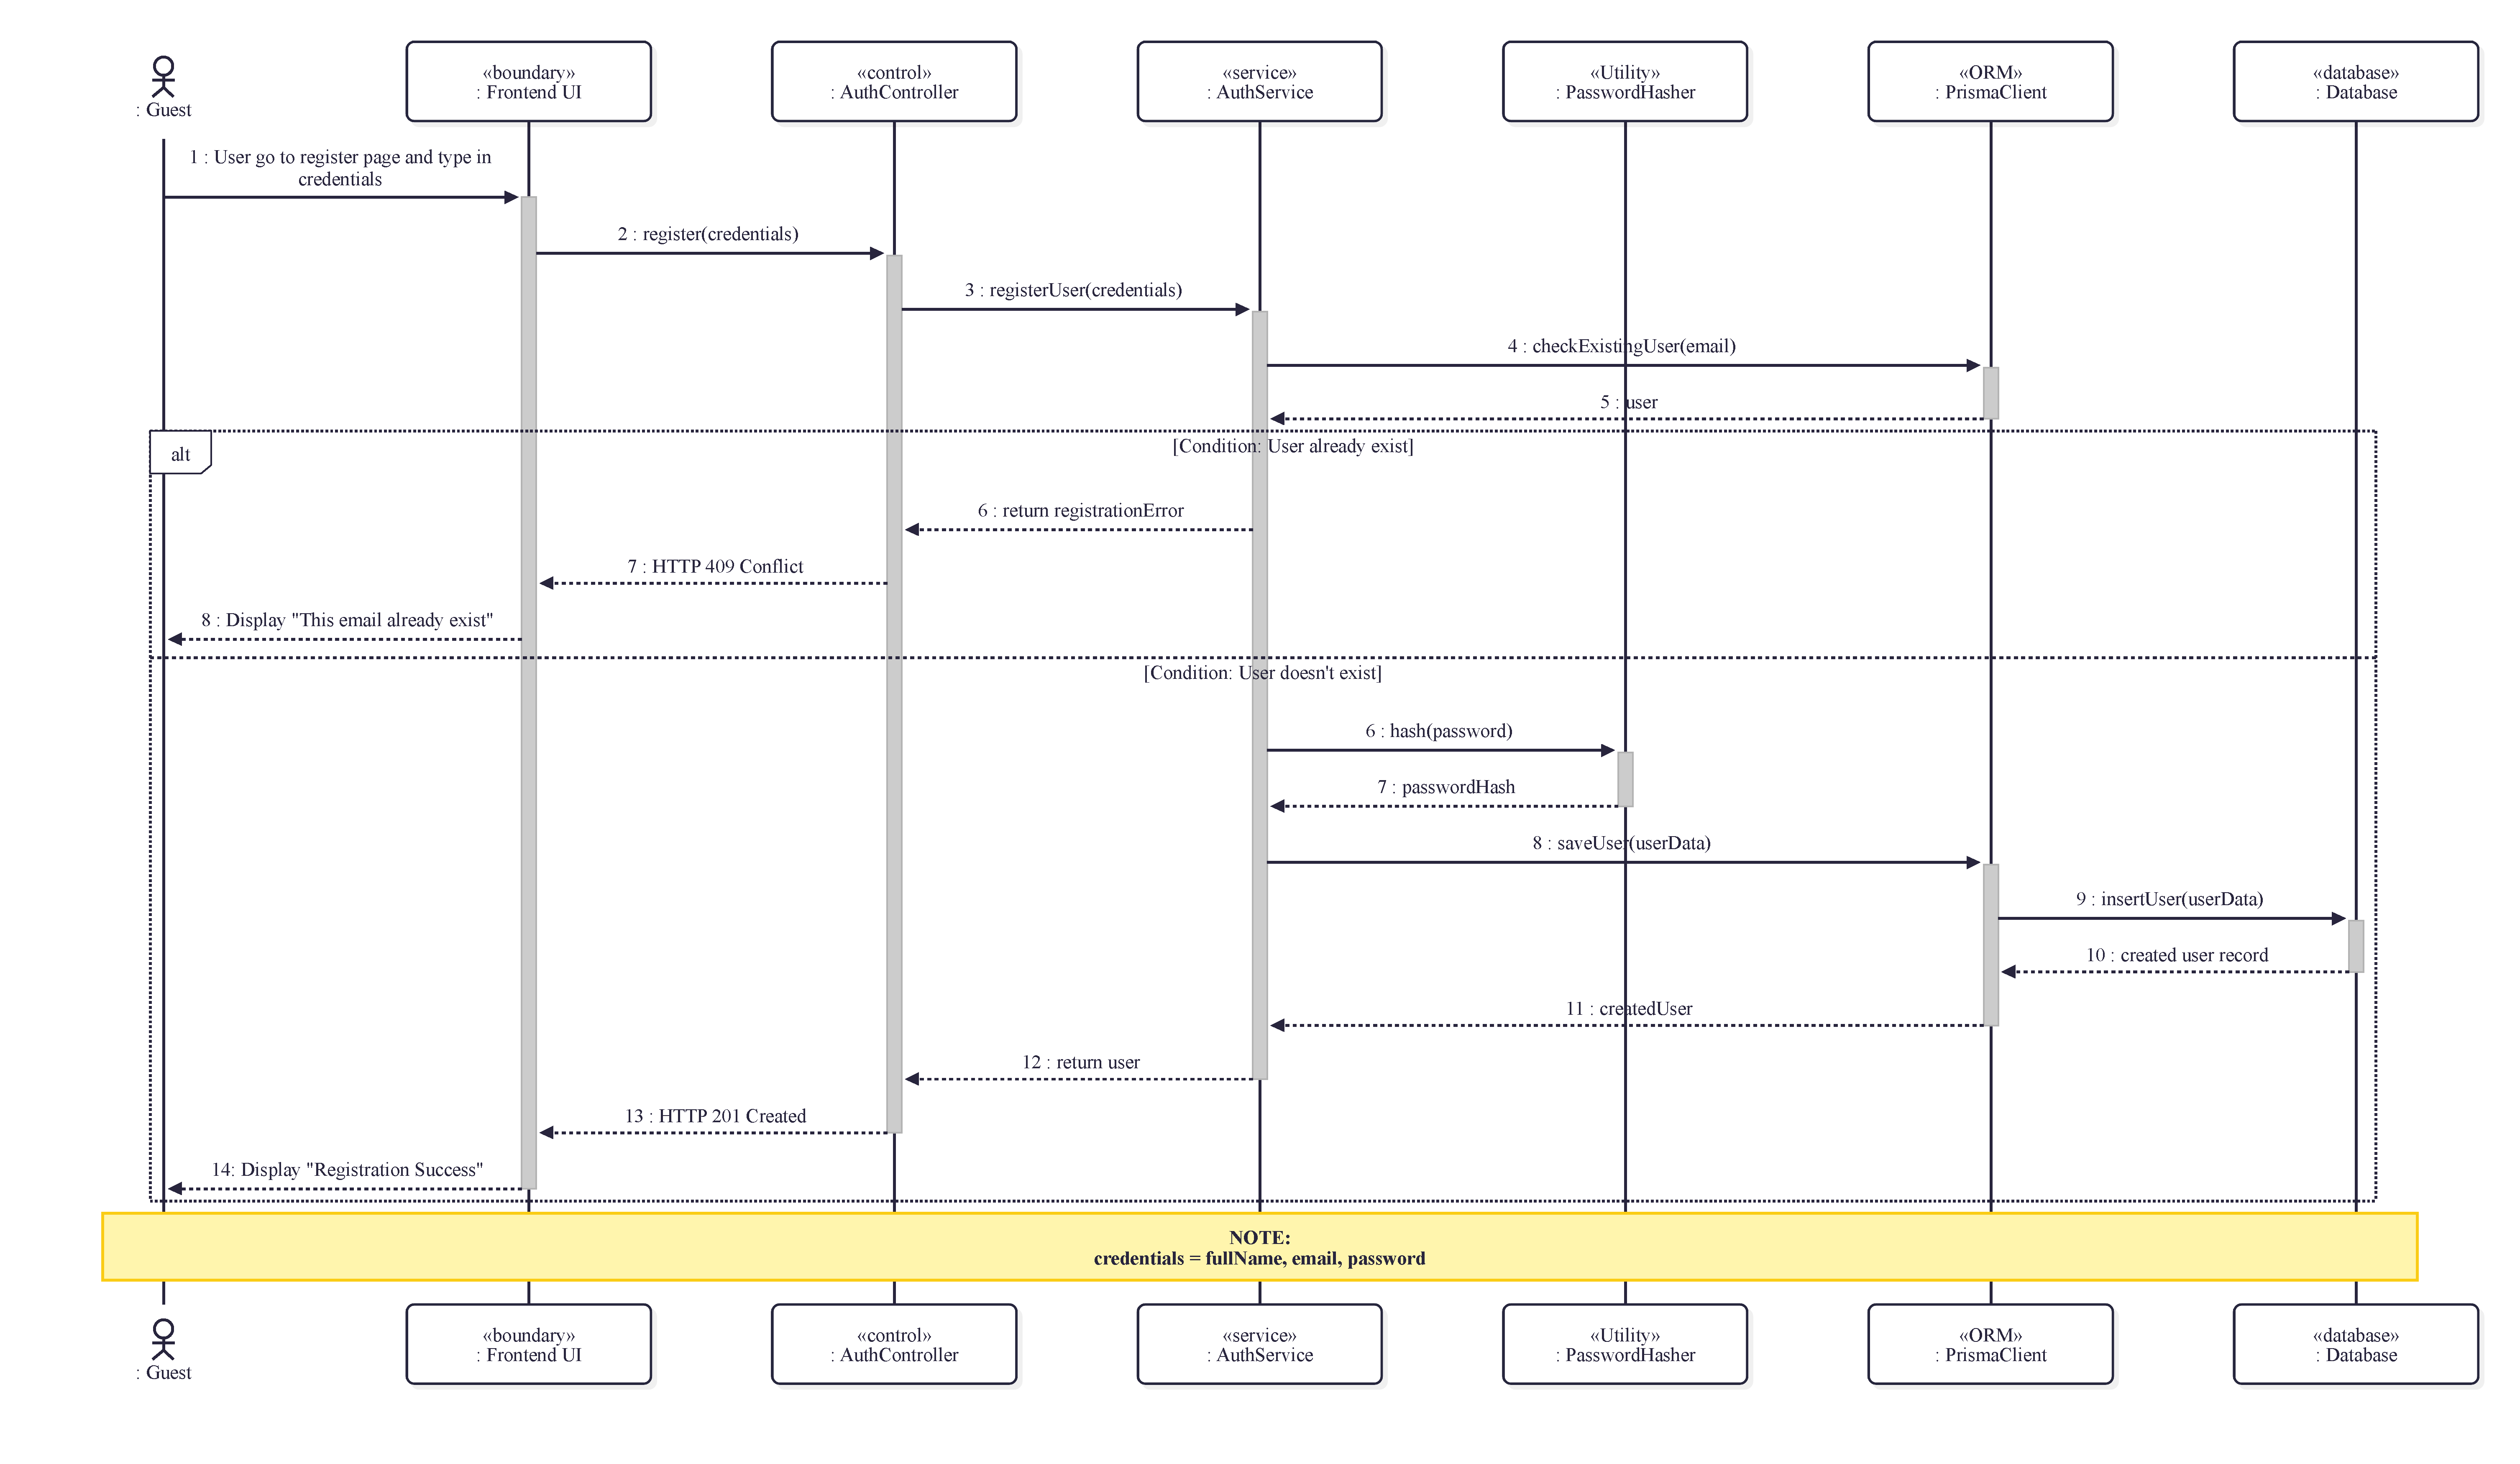
\includegraphics[width=0.9\linewidth]{diagrams/exported/2Auth/SD-Auth01-Register.pdf}
	\caption{Sequence Diagram: Register.}
	\label{diagram:sd-auth-register}
\end{figure}

\begin{figure}[H]
	\centering
	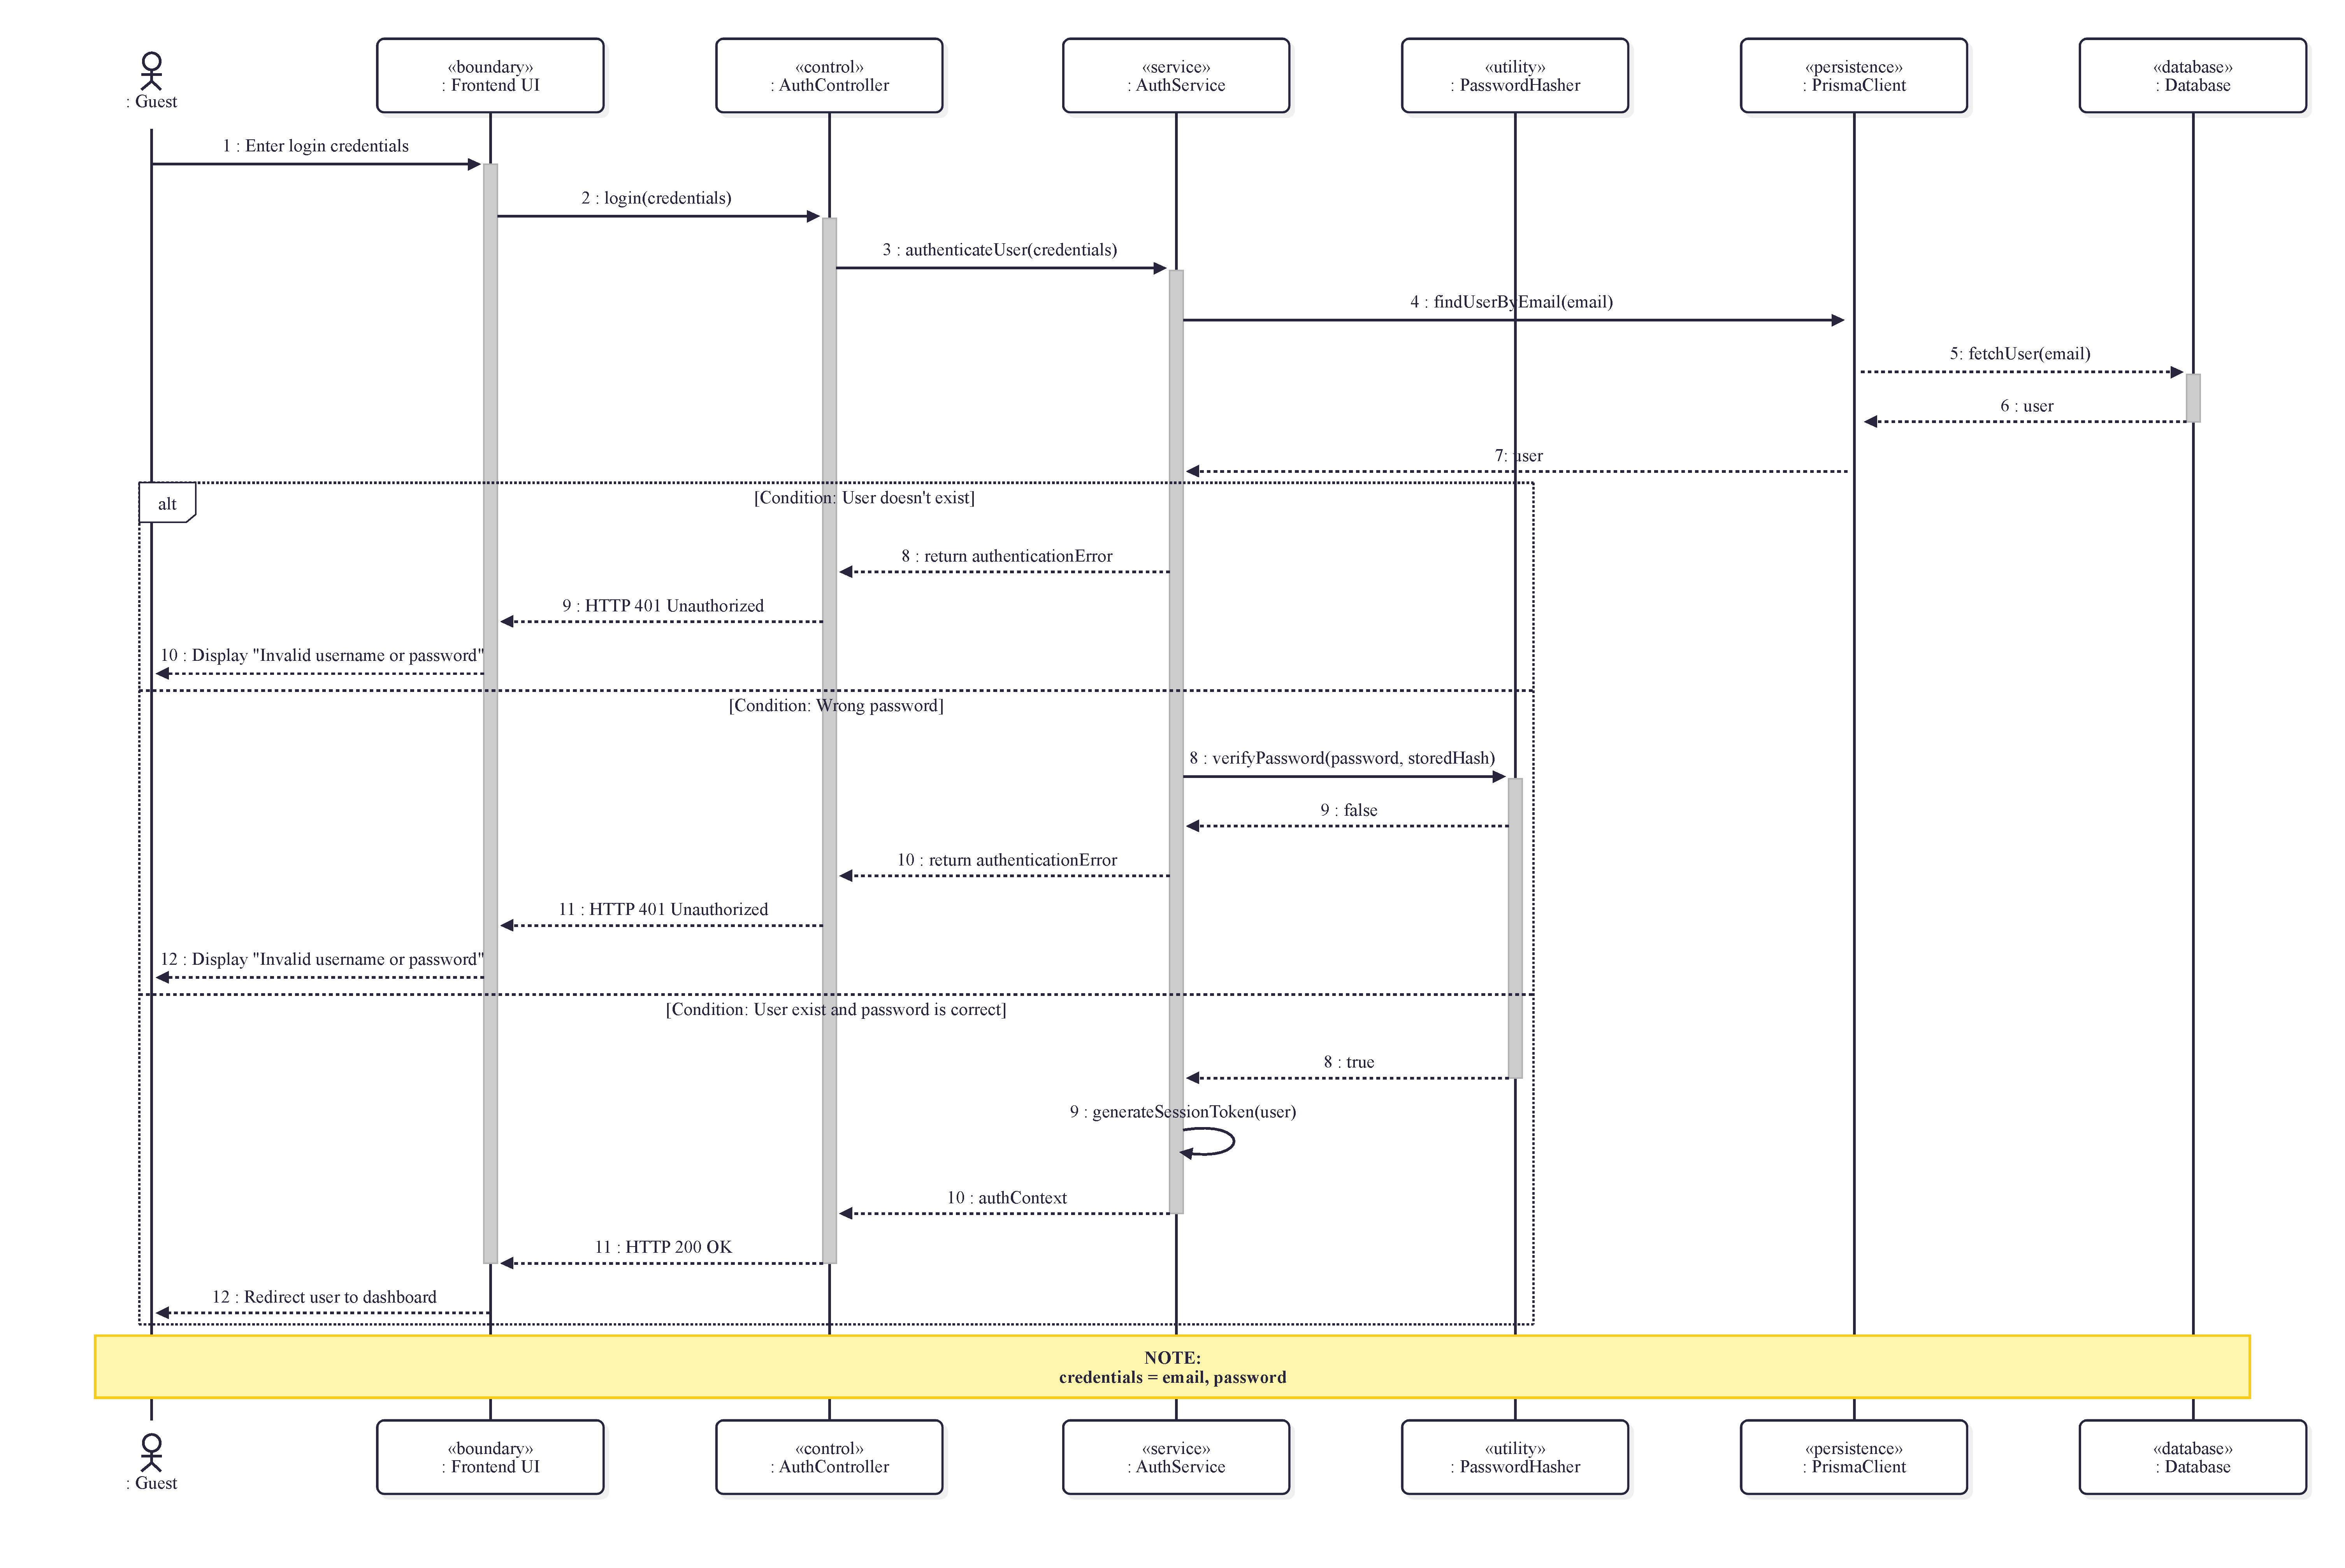
\includegraphics[width=0.9\linewidth]{diagrams/exported/2Auth/SD-Auth02-Login.pdf}
	\caption{Sequence Diagram: Login.}
	\label{diagram:sd-auth-login}
\end{figure}

\begin{figure}[H]
	\centering
	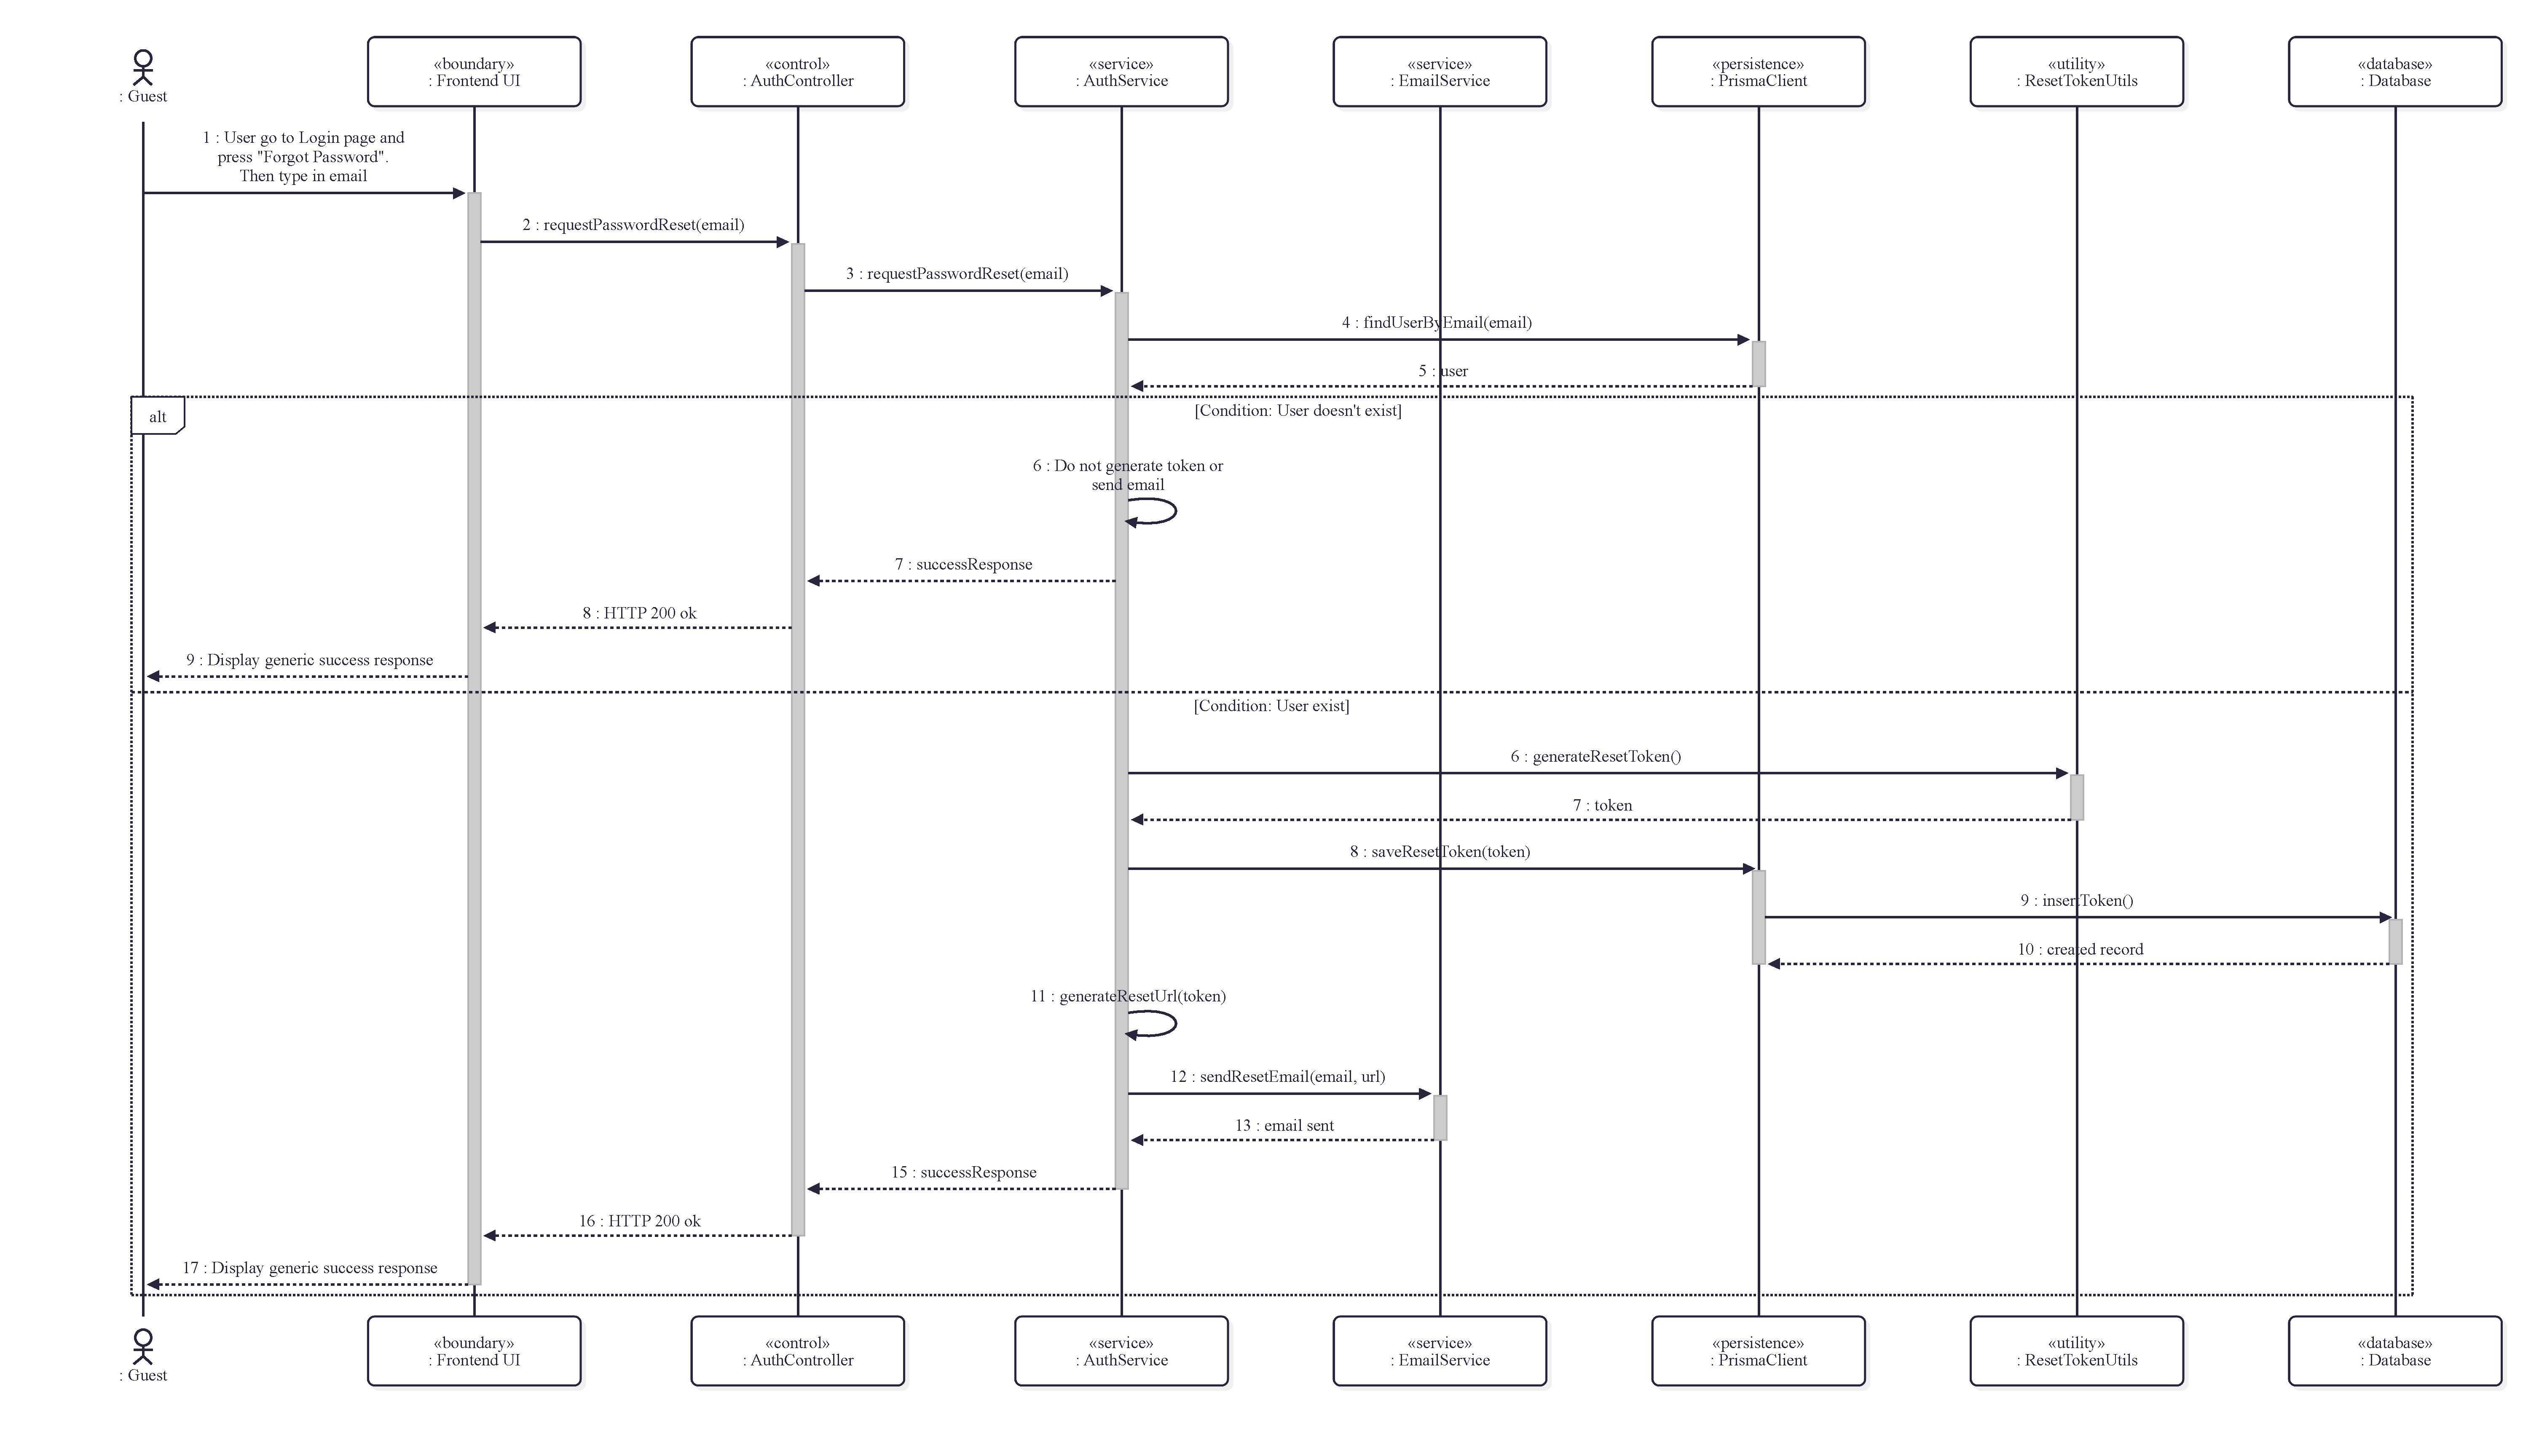
\includegraphics[width=0.9\linewidth]{diagrams/exported/2Auth/SD-Auth04-Forgot-Password.pdf}
	\caption{Sequence Diagram: Forgot Password.}
	\label{diagram:sd-auth-forgot-password}
\end{figure}

\begin{figure}[H]
	\centering
	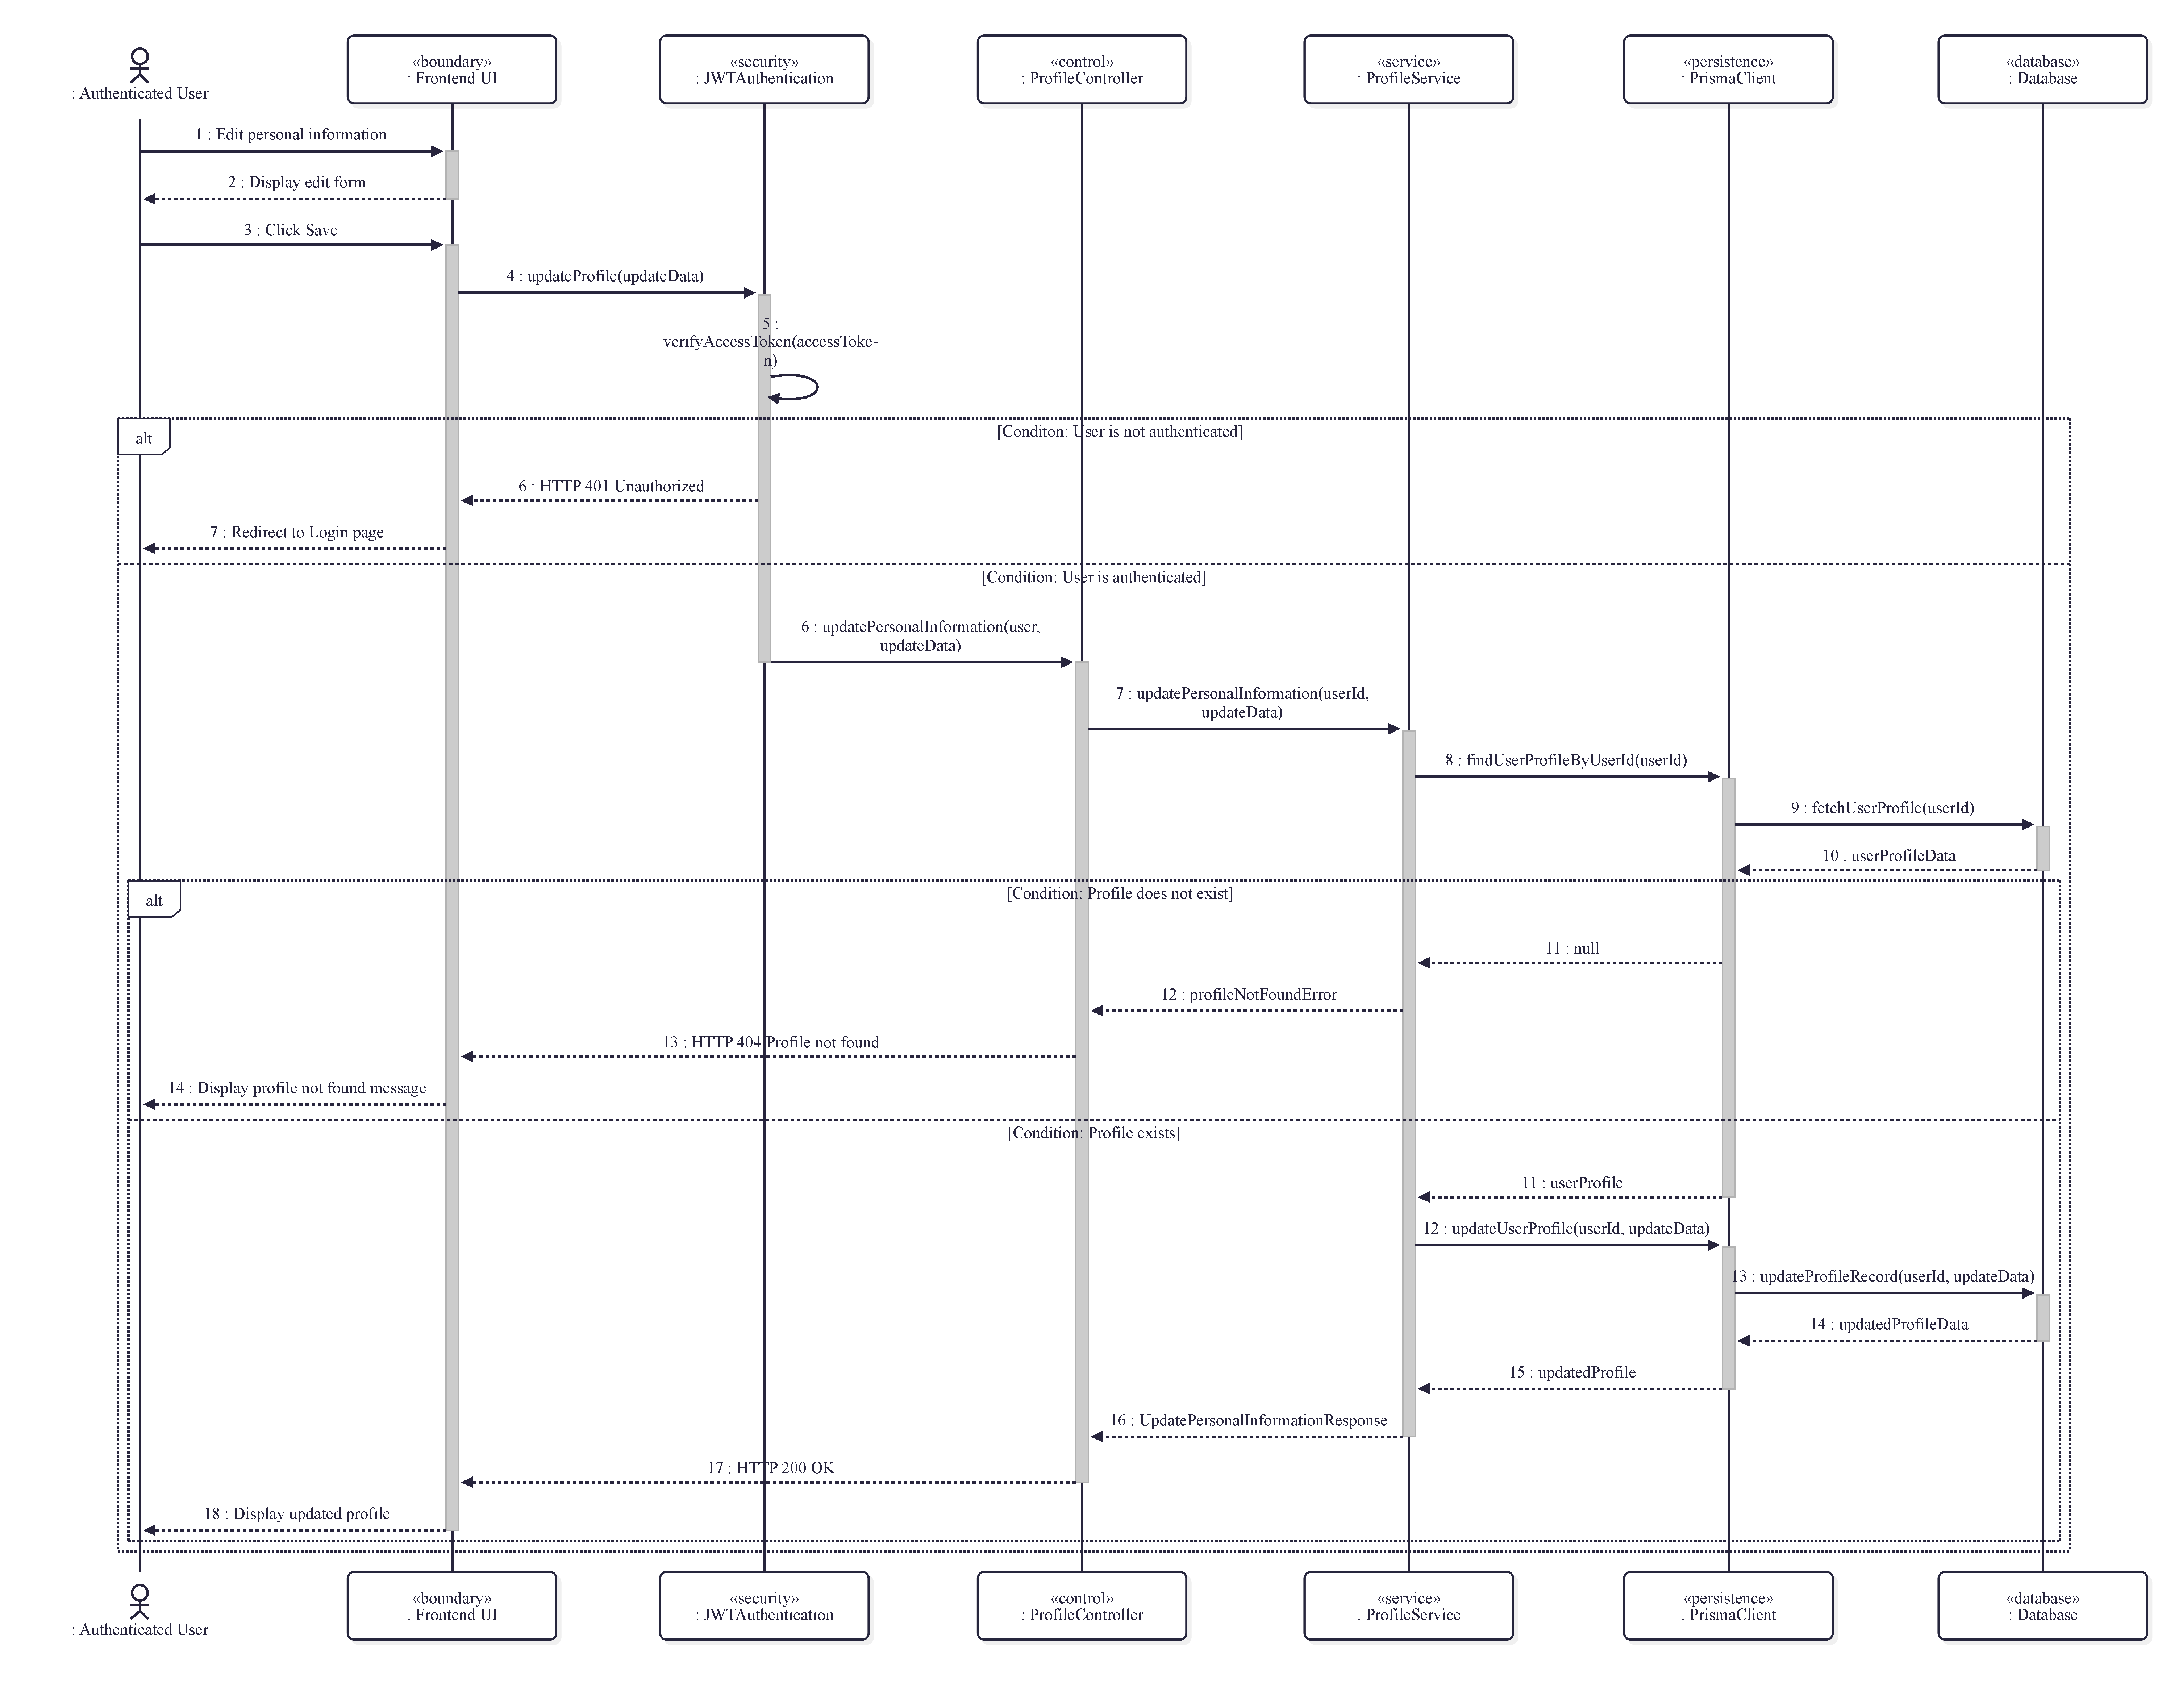
\includegraphics[width=0.9\linewidth]{diagrams/exported/3Profile/SD-Profile01-Update-Personal-Information.pdf}
	\caption{Sequence Diagram: Update Personal Information.}
	\label{diagram:sd-profile-update}
\end{figure}

\begin{figure}[H]
	\centering
	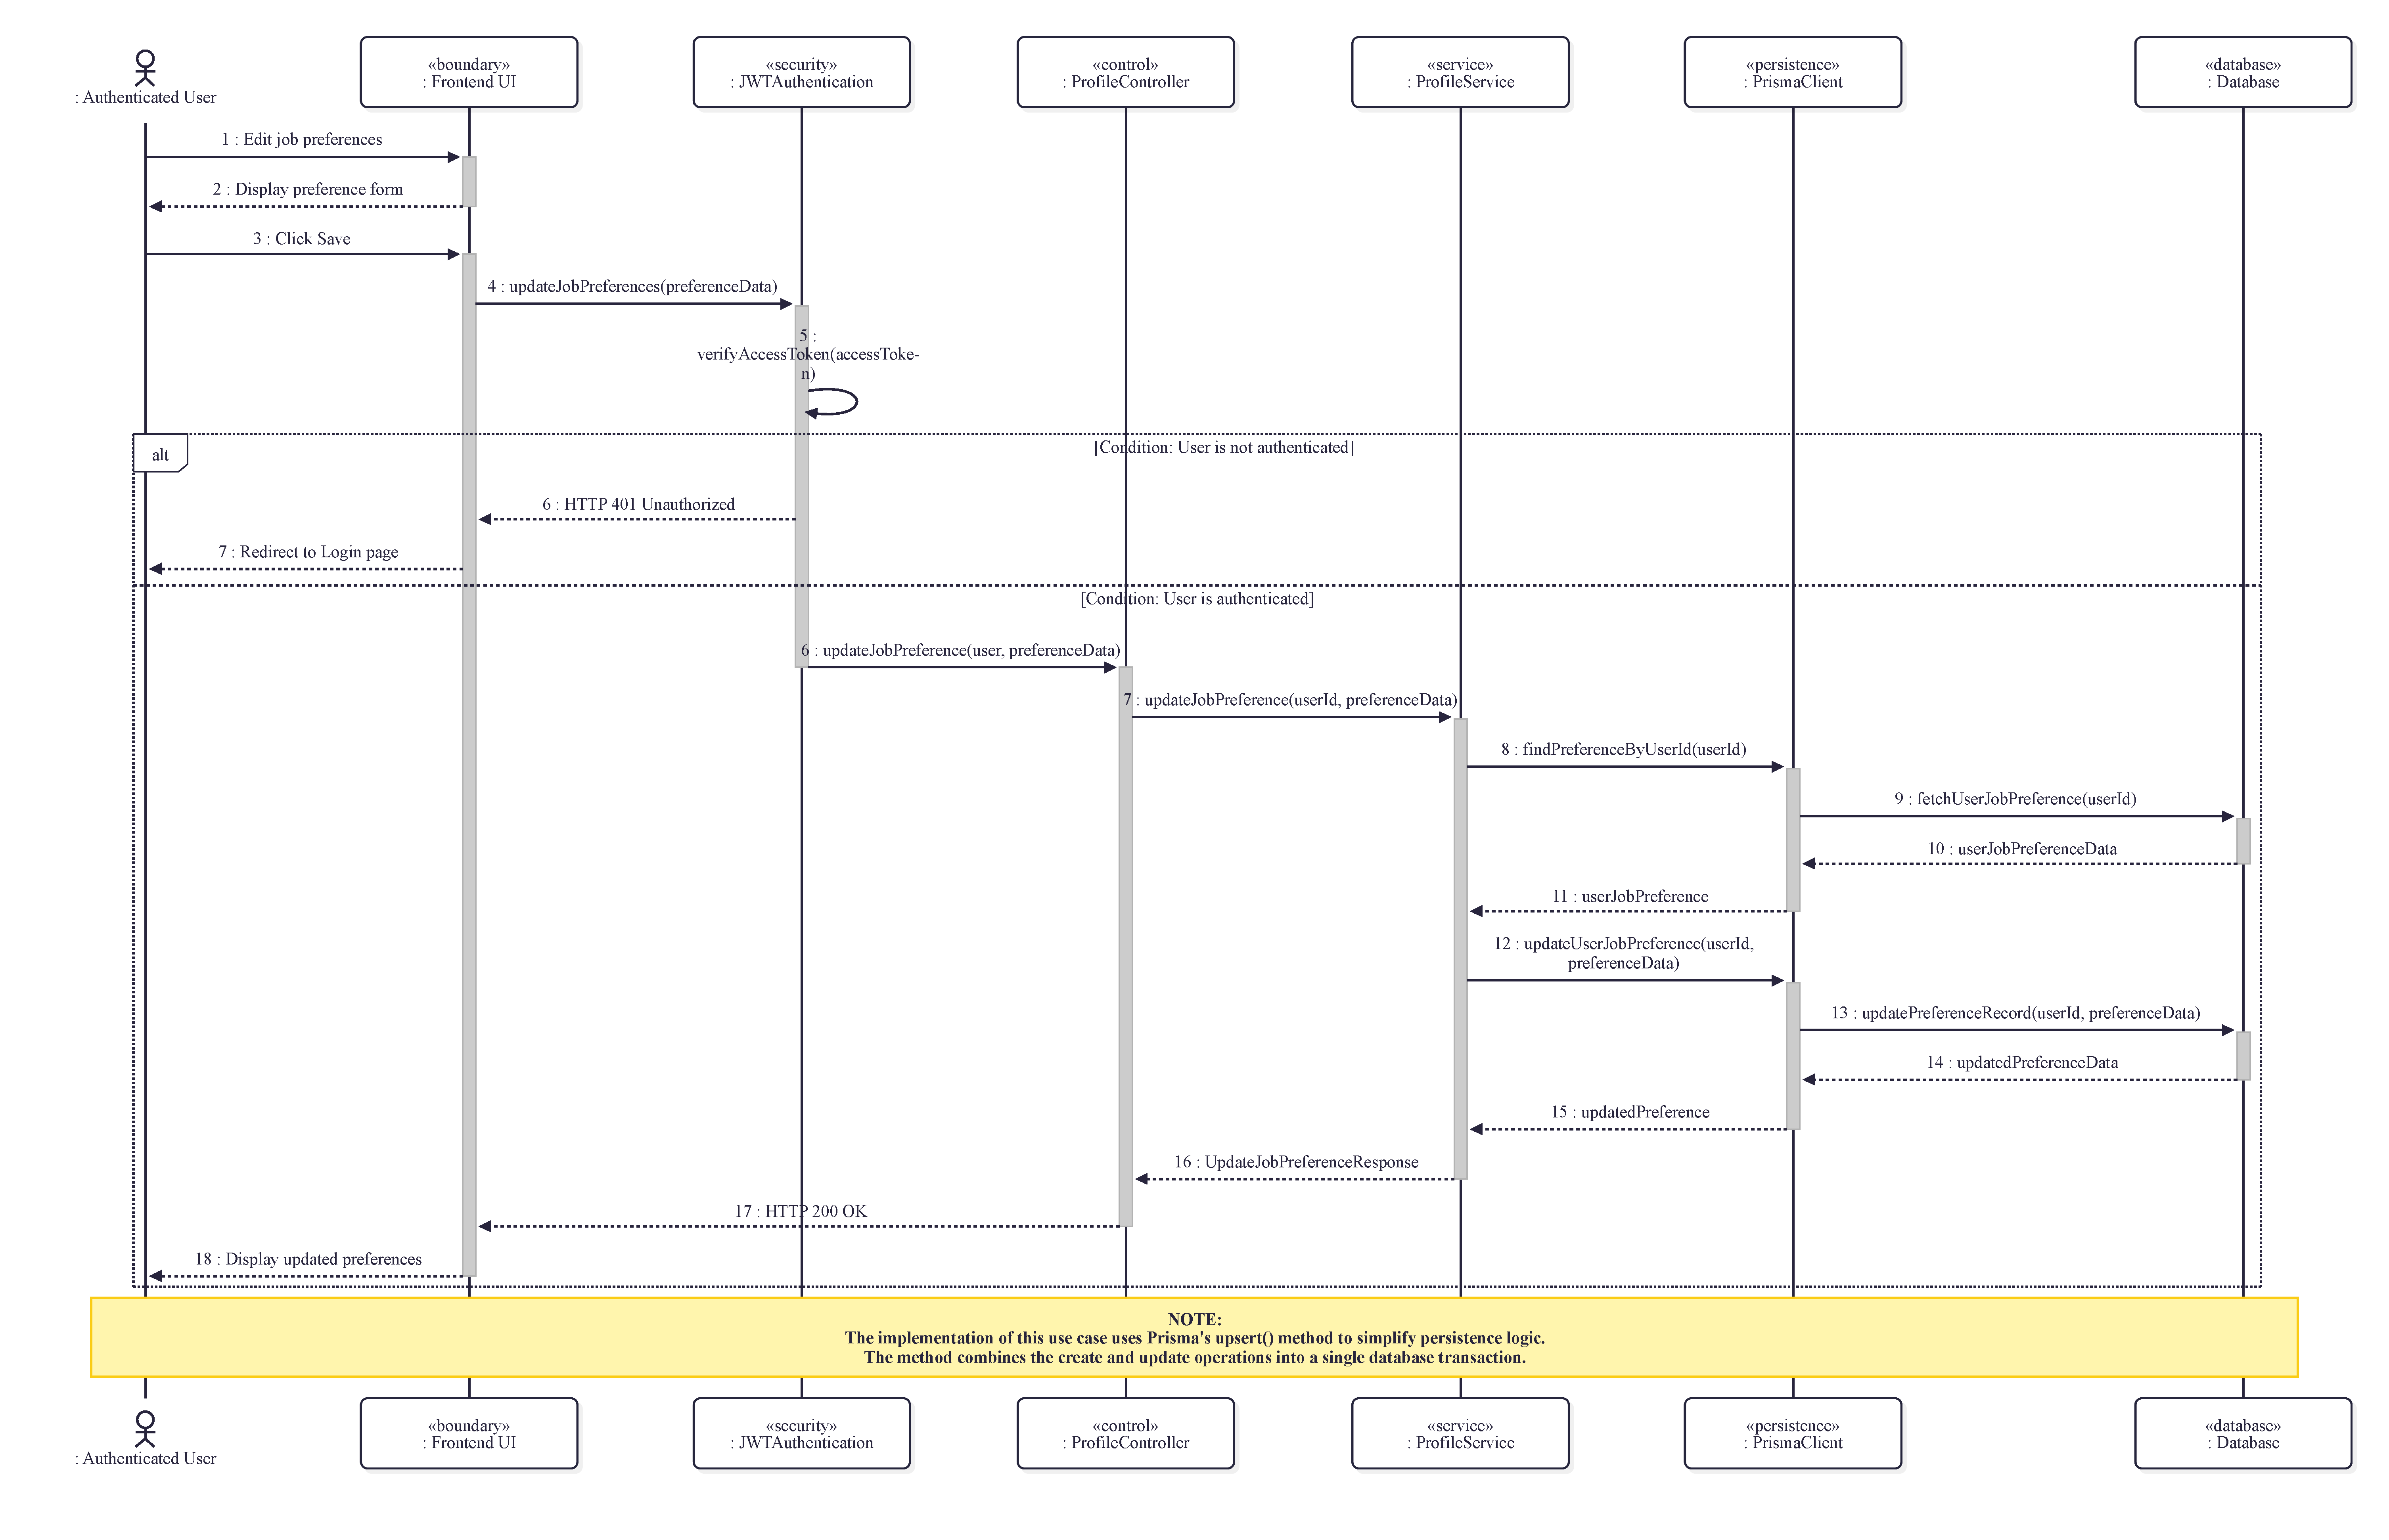
\includegraphics[width=0.9\linewidth]{diagrams/exported/3Profile/SD-Profile02-Update-Job-Preferences.pdf}
	\caption{Sequence Diagram: Update Job Preferences.}
	\label{diagram:sd-profile-preferences}
\end{figure}

\begin{figure}[H]
	\centering
	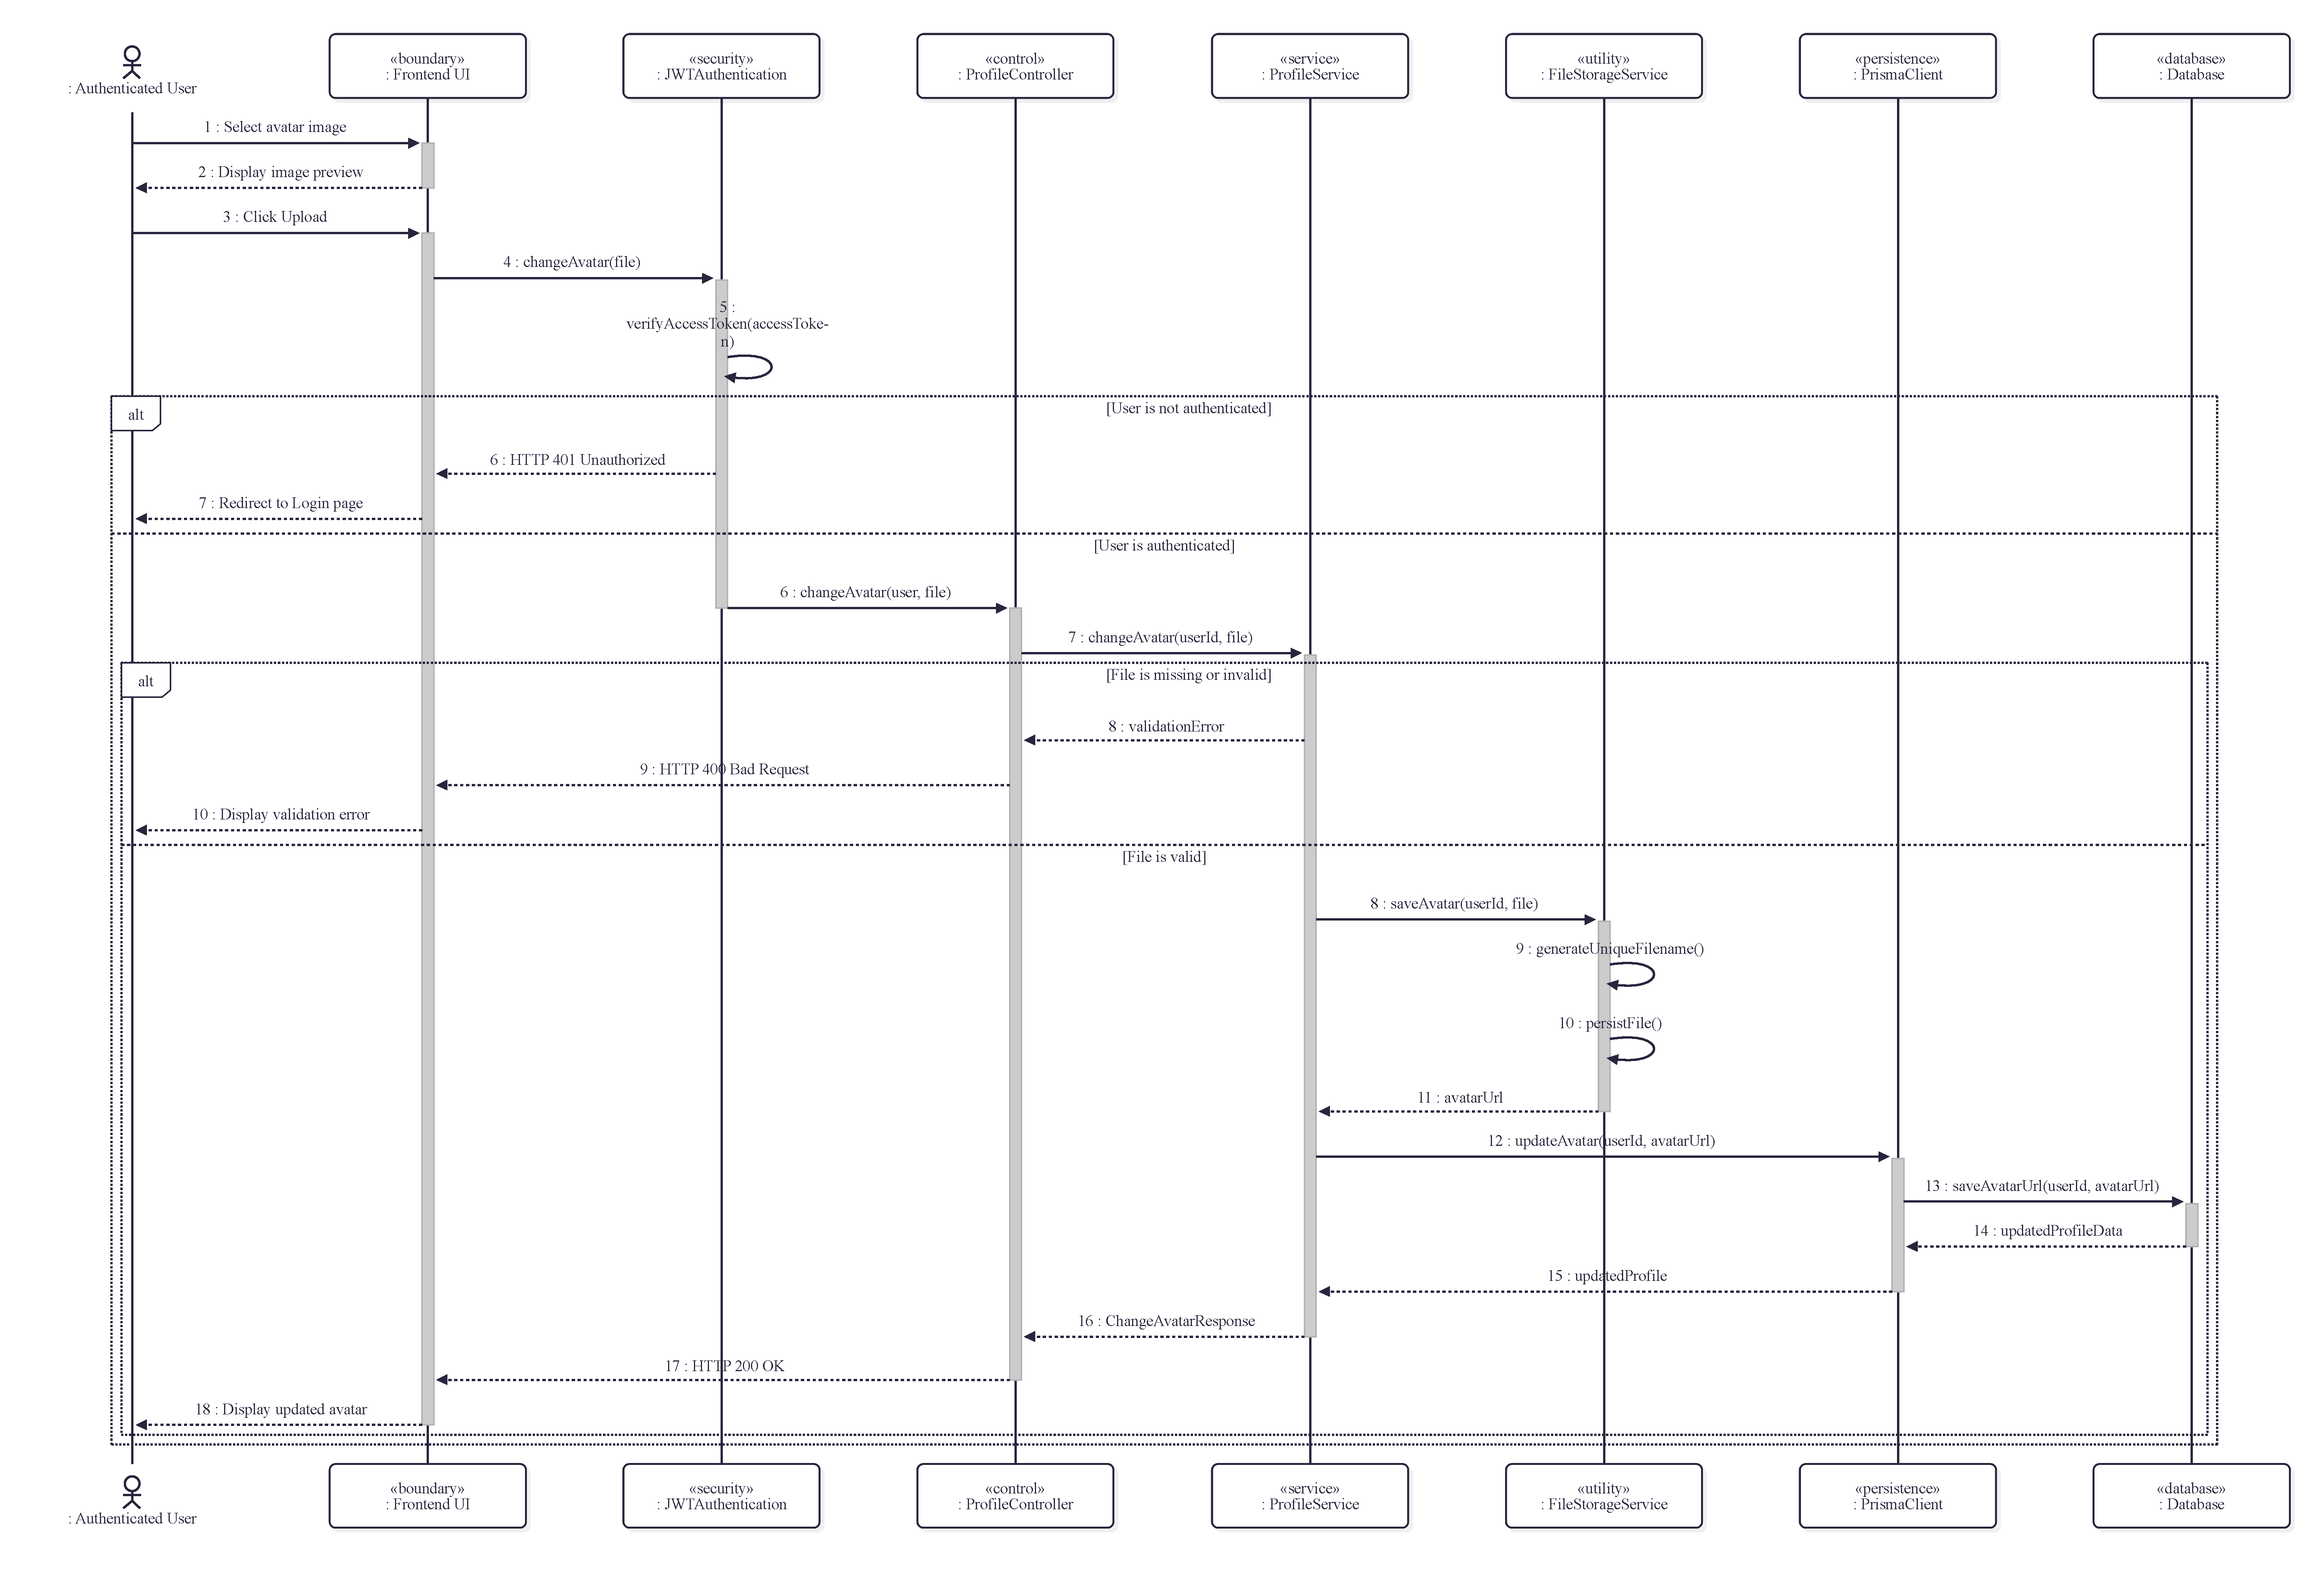
\includegraphics[width=0.9\linewidth]{diagrams/exported/3Profile/SD-Profile03-Change-Avatar.pdf}
	\caption{Sequence Diagram: Change Avatar.}
	\label{diagram:sd-profile-avatar}
\end{figure}

\begin{figure}[H]
	\centering
	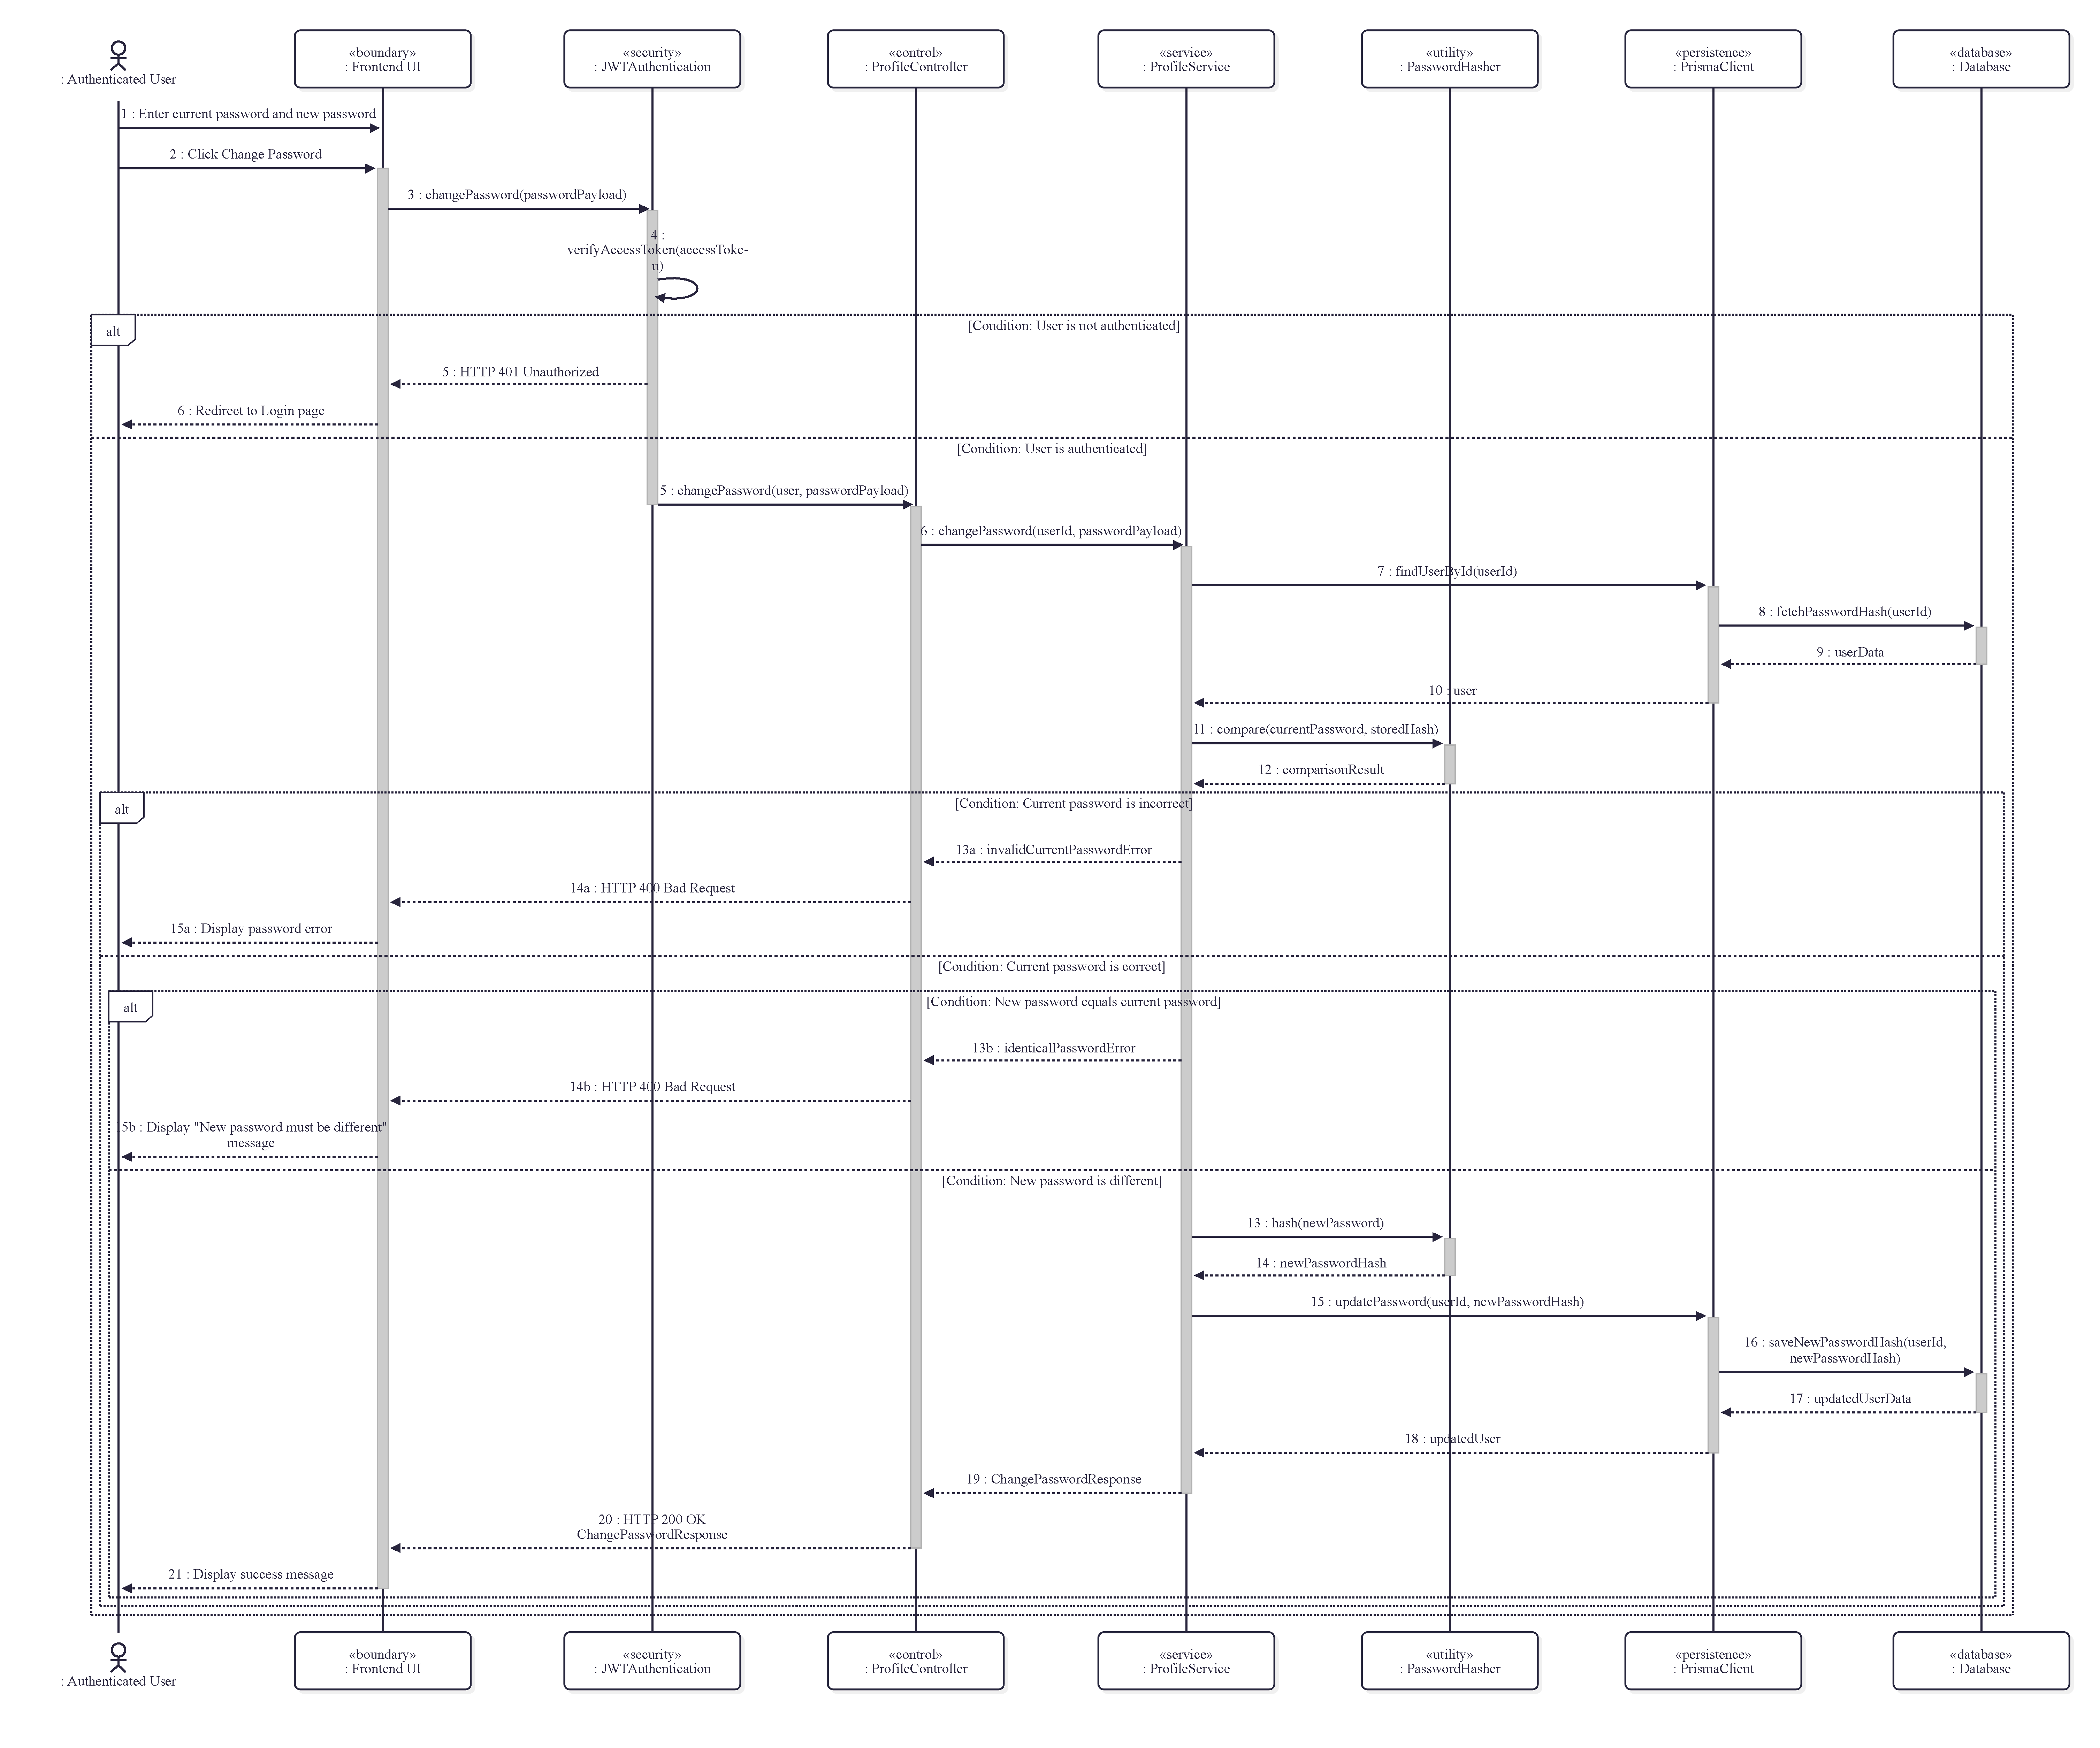
\includegraphics[width=0.9\linewidth]{diagrams/exported/3Profile/SD-Profile04-Change-Password.pdf}
	\caption{Sequence Diagram: Change Password.}
	\label{diagram:sd-profile-password}
\end{figure}

\begin{figure}[H]
	\centering
	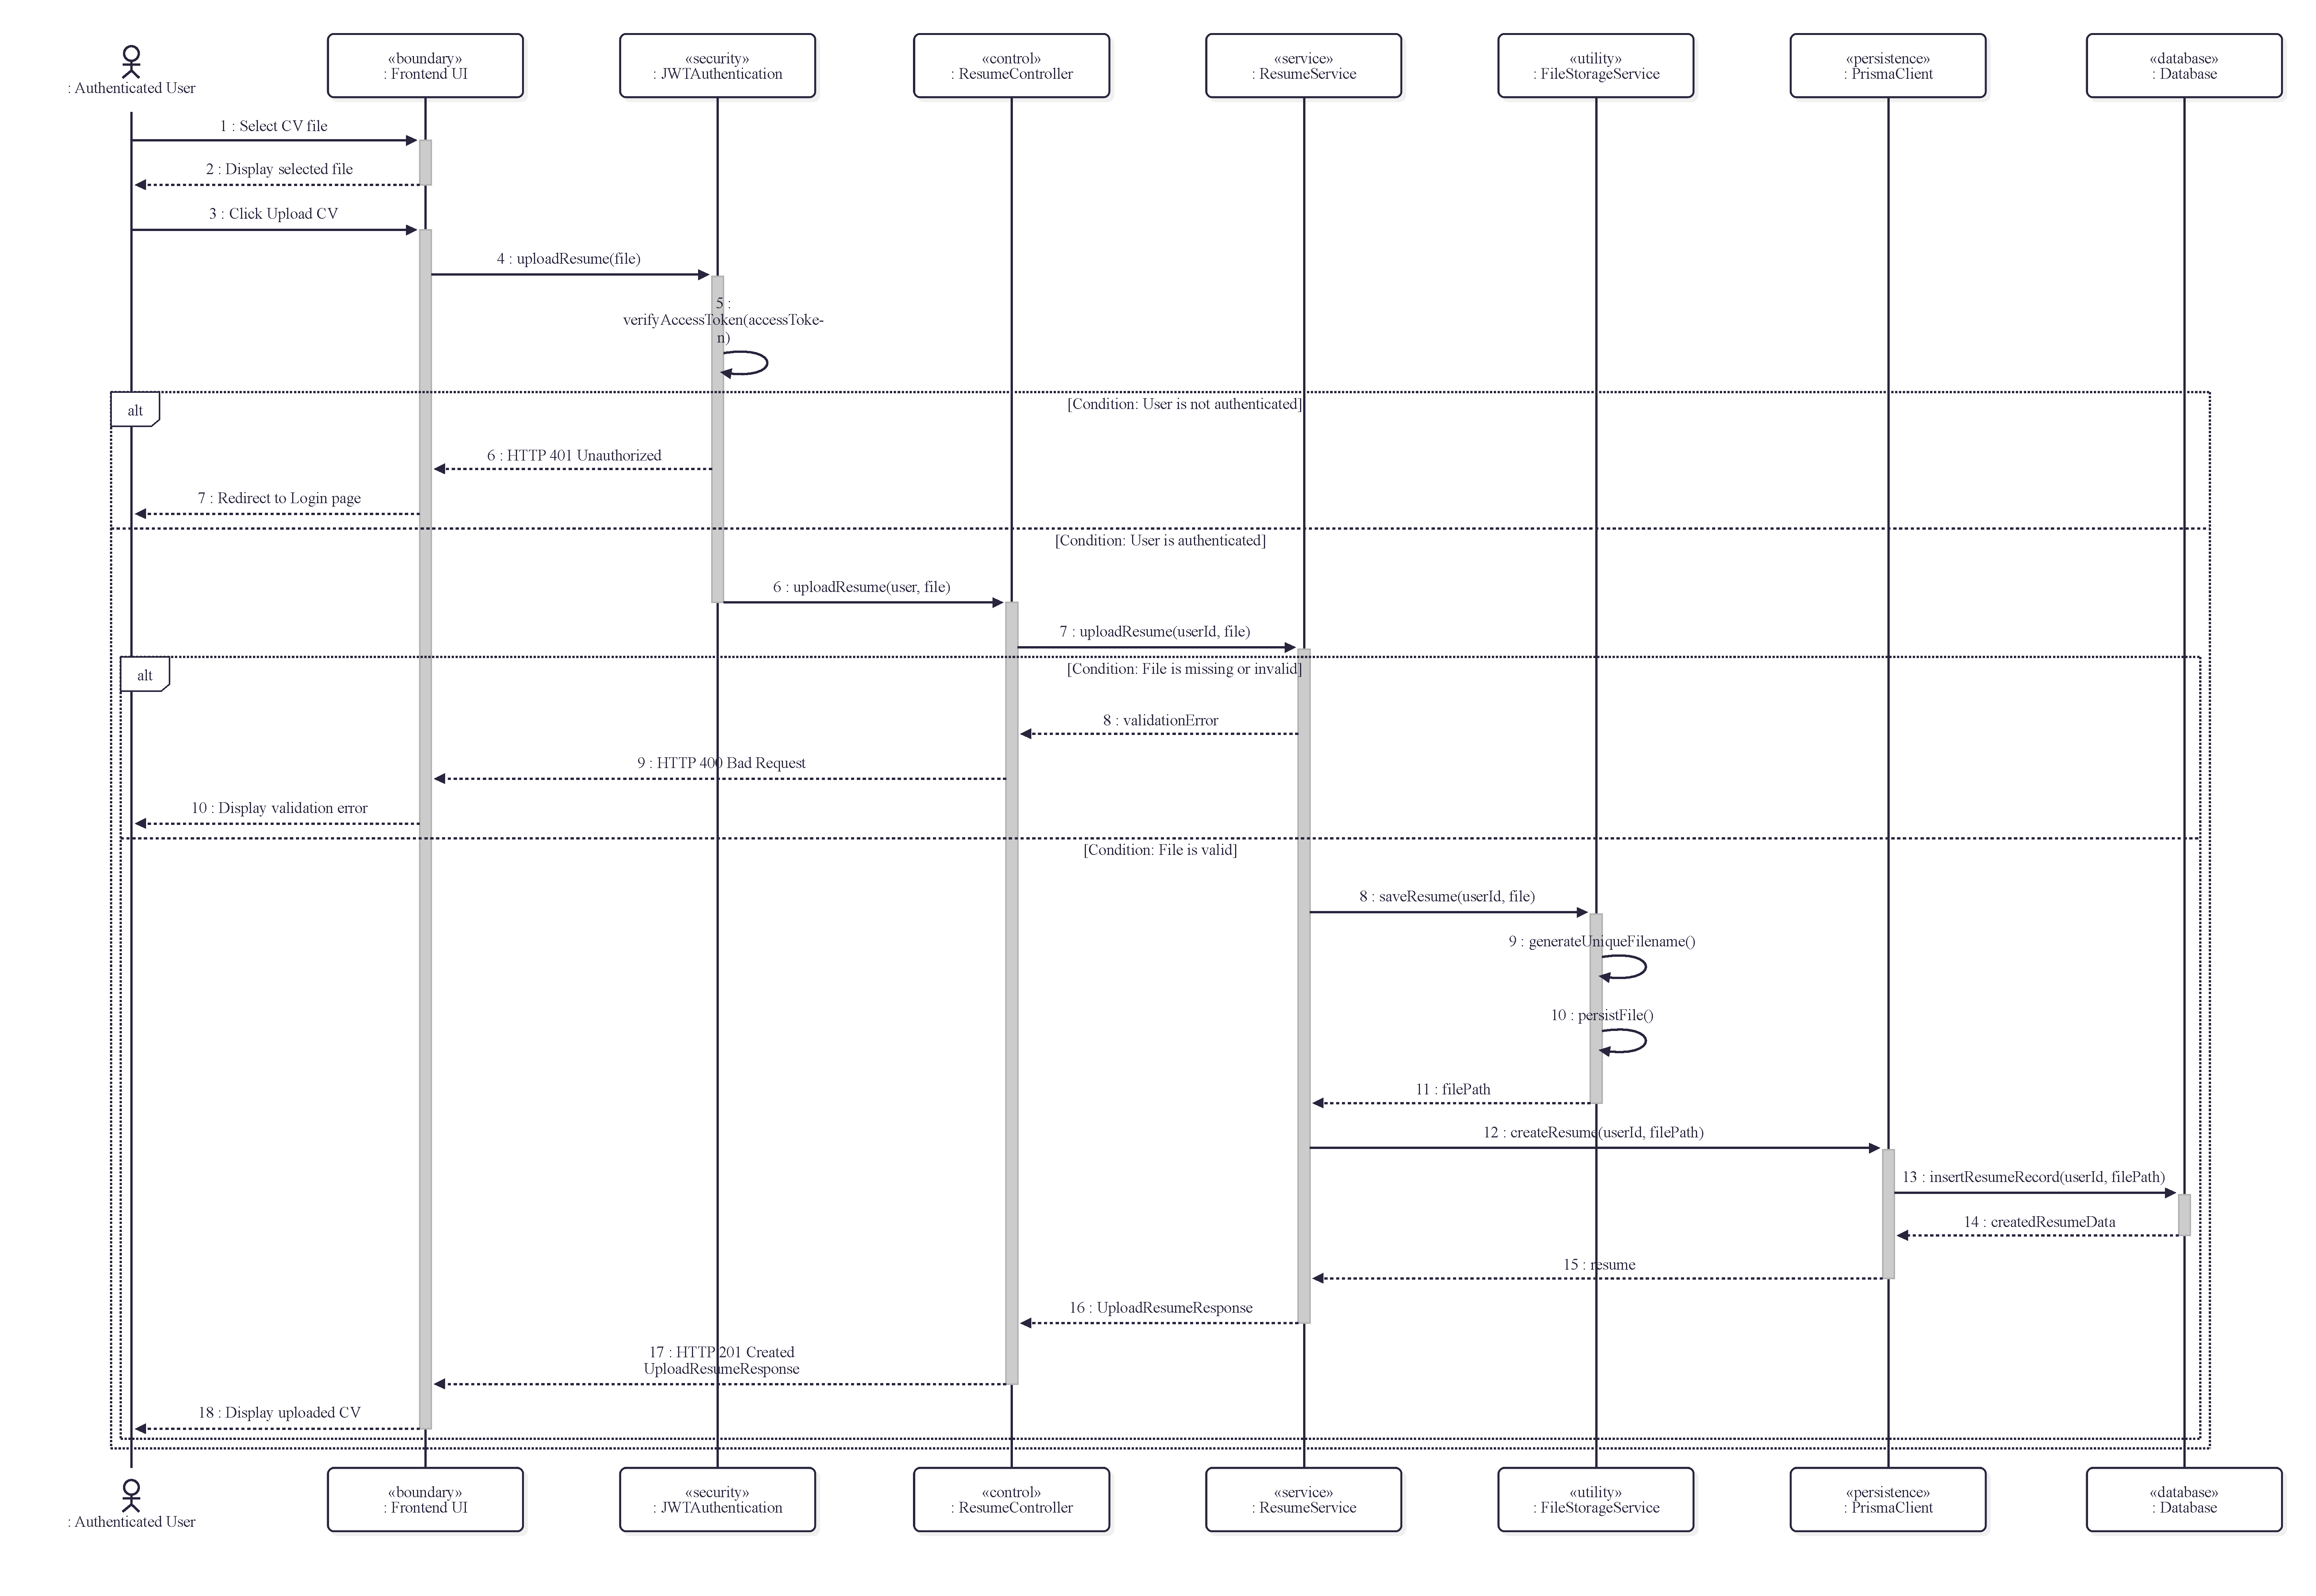
\includegraphics[width=0.9\linewidth]{diagrams/exported/4Resume/SD-Profile05-Upload-CV.pdf}
	\caption{Sequence Diagram: Upload CV.}
	\label{diagram:sd-resume-upload}
\end{figure}

\section{Public}

\begin{figure}[H]
	\centering
	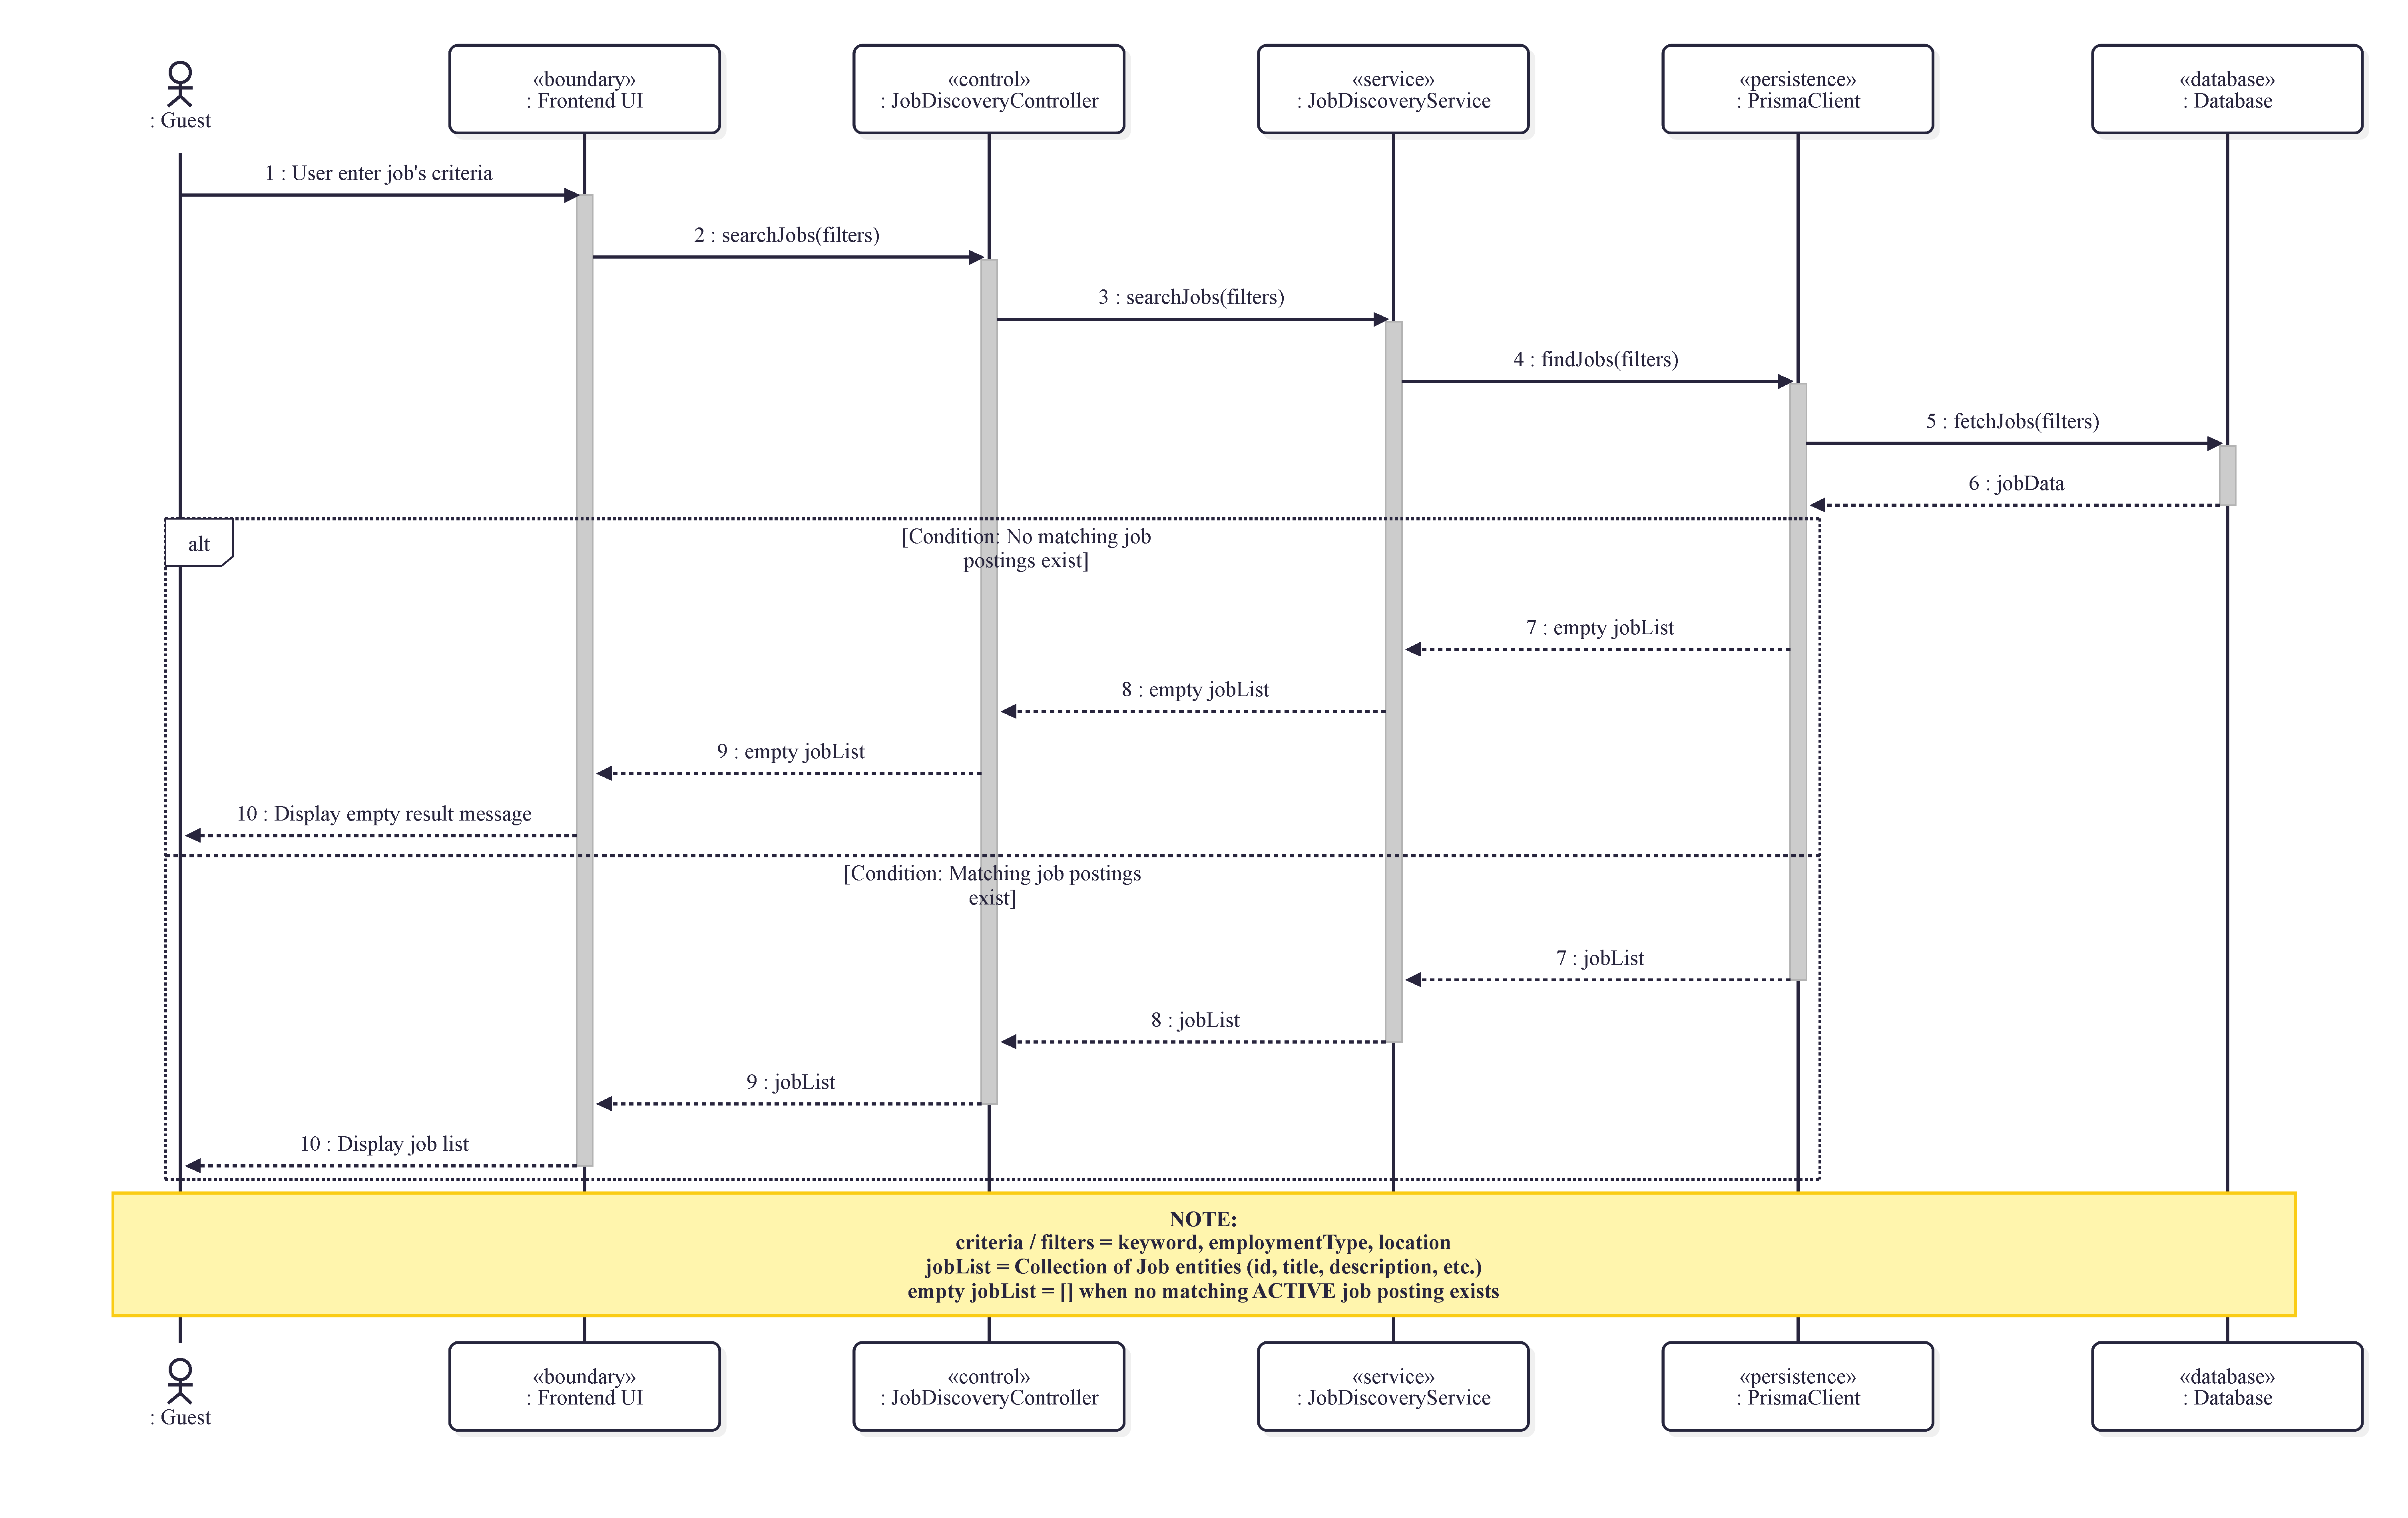
\includegraphics[width=0.9\linewidth]{diagrams/exported/1Public/SD-Public!01-Search-Jobs.pdf}
	\caption{Sequence Diagram: Search Jobs.}
	\label{diagram:sd-public-search}
\end{figure}

\begin{figure}[H]
	\centering
	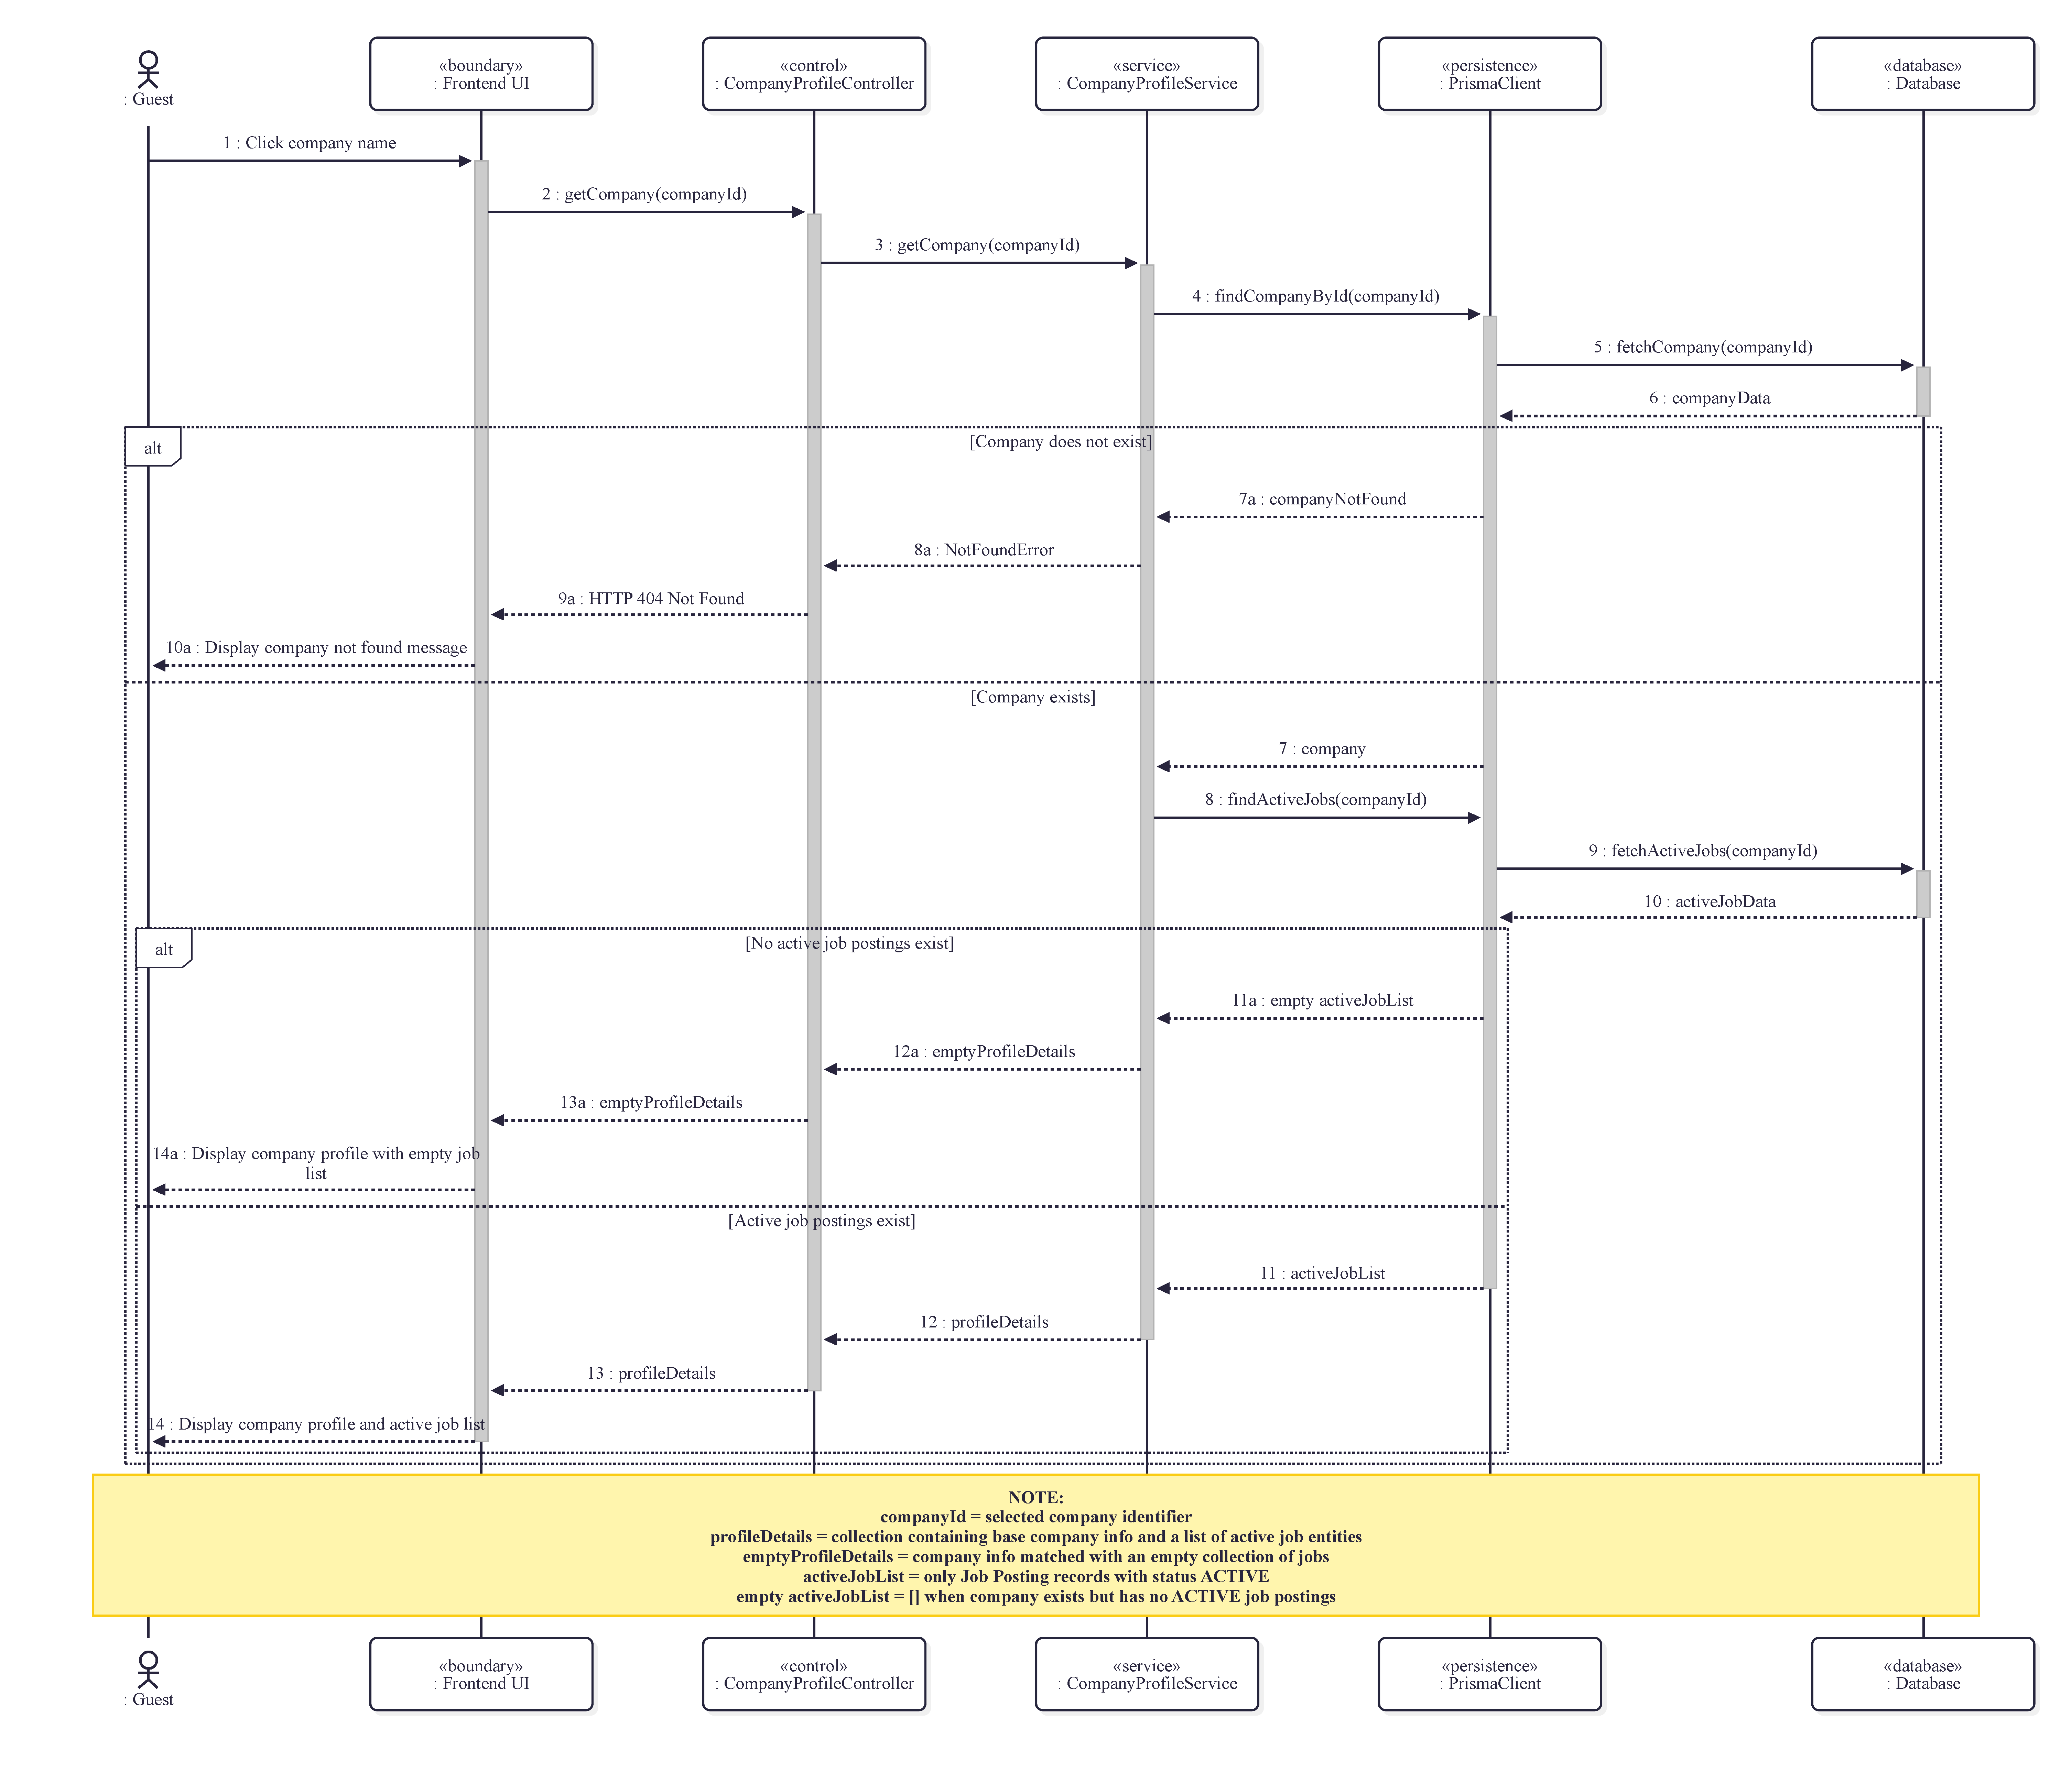
\includegraphics[width=0.9\linewidth]{diagrams/exported/1Public/SD-Public!02-View-Company-Profile.pdf}
	\caption{Sequence Diagram: View Company Profile.}
	\label{diagram:sd-public-company}
\end{figure}

\section{Back Office}

\begin{figure}[H]
	\centering
	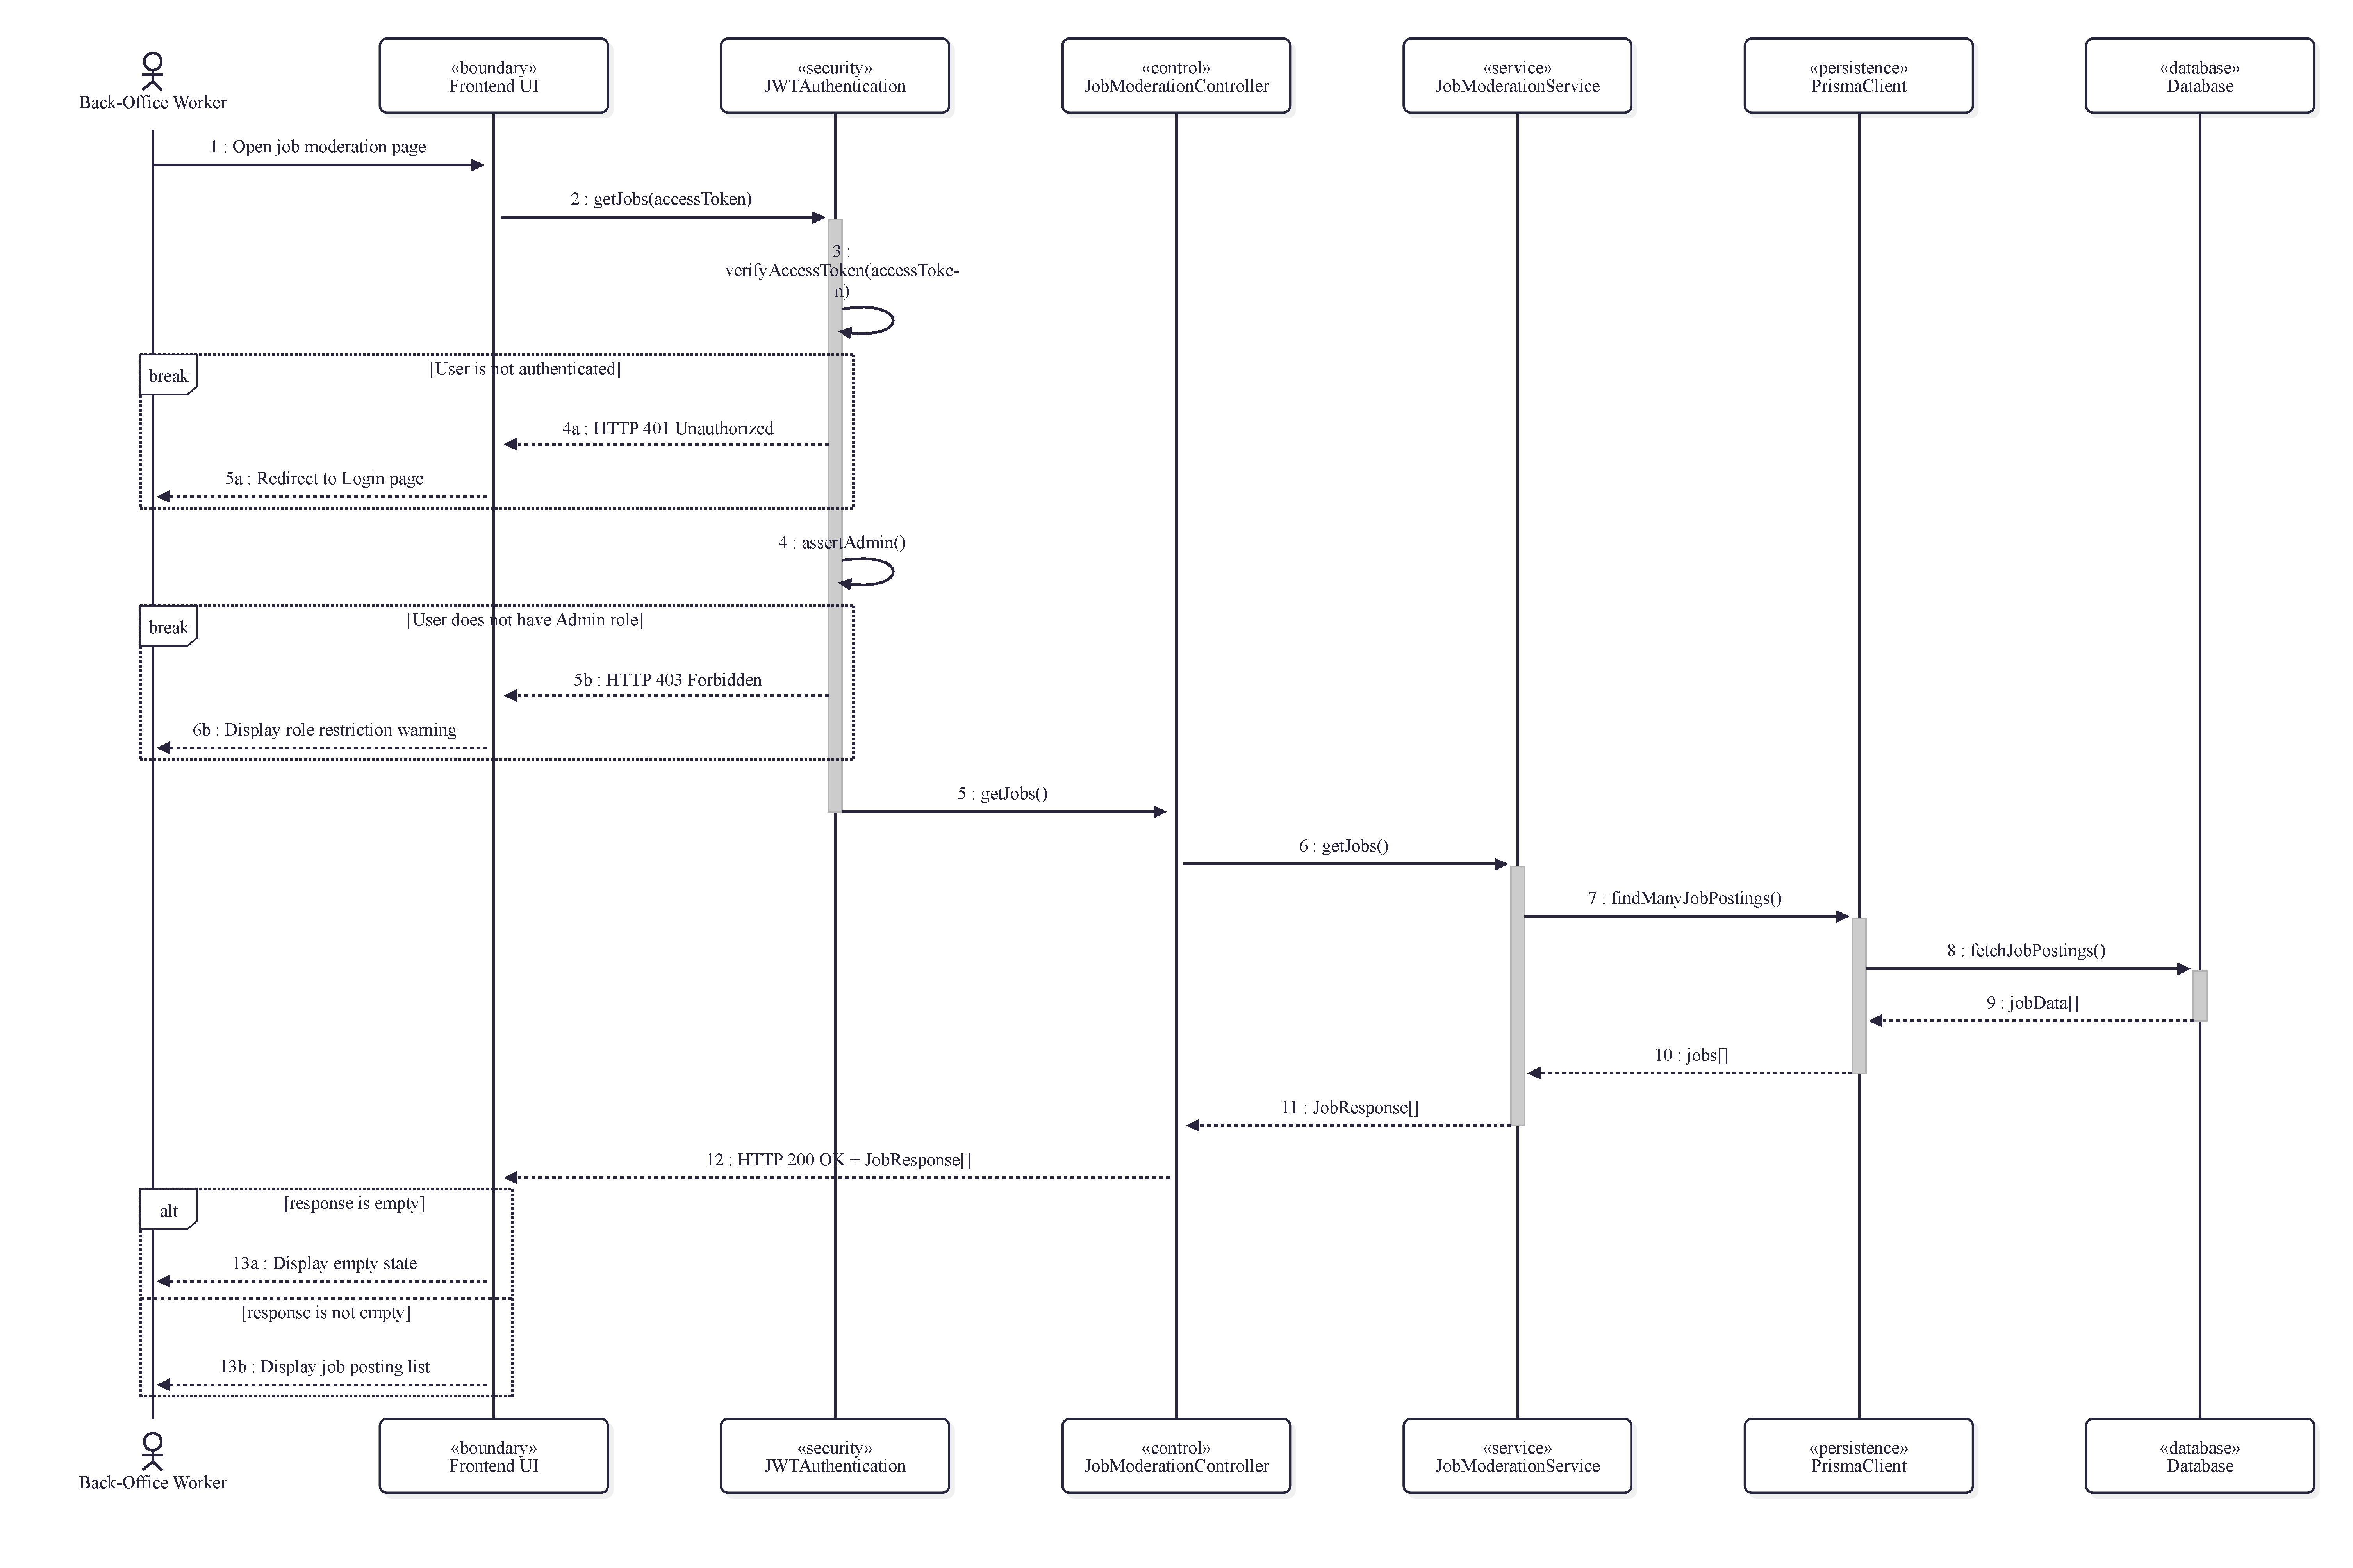
\includegraphics[width=0.9\linewidth]{diagrams/exported/7BackOffice/SD-Admin01-Get-Job-Postings-List.pdf}
	\caption{Sequence Diagram: Get Job Postings List.}
	\label{diagram:sd-admin-jobs-list}
\end{figure}

\begin{figure}[H]
	\centering
	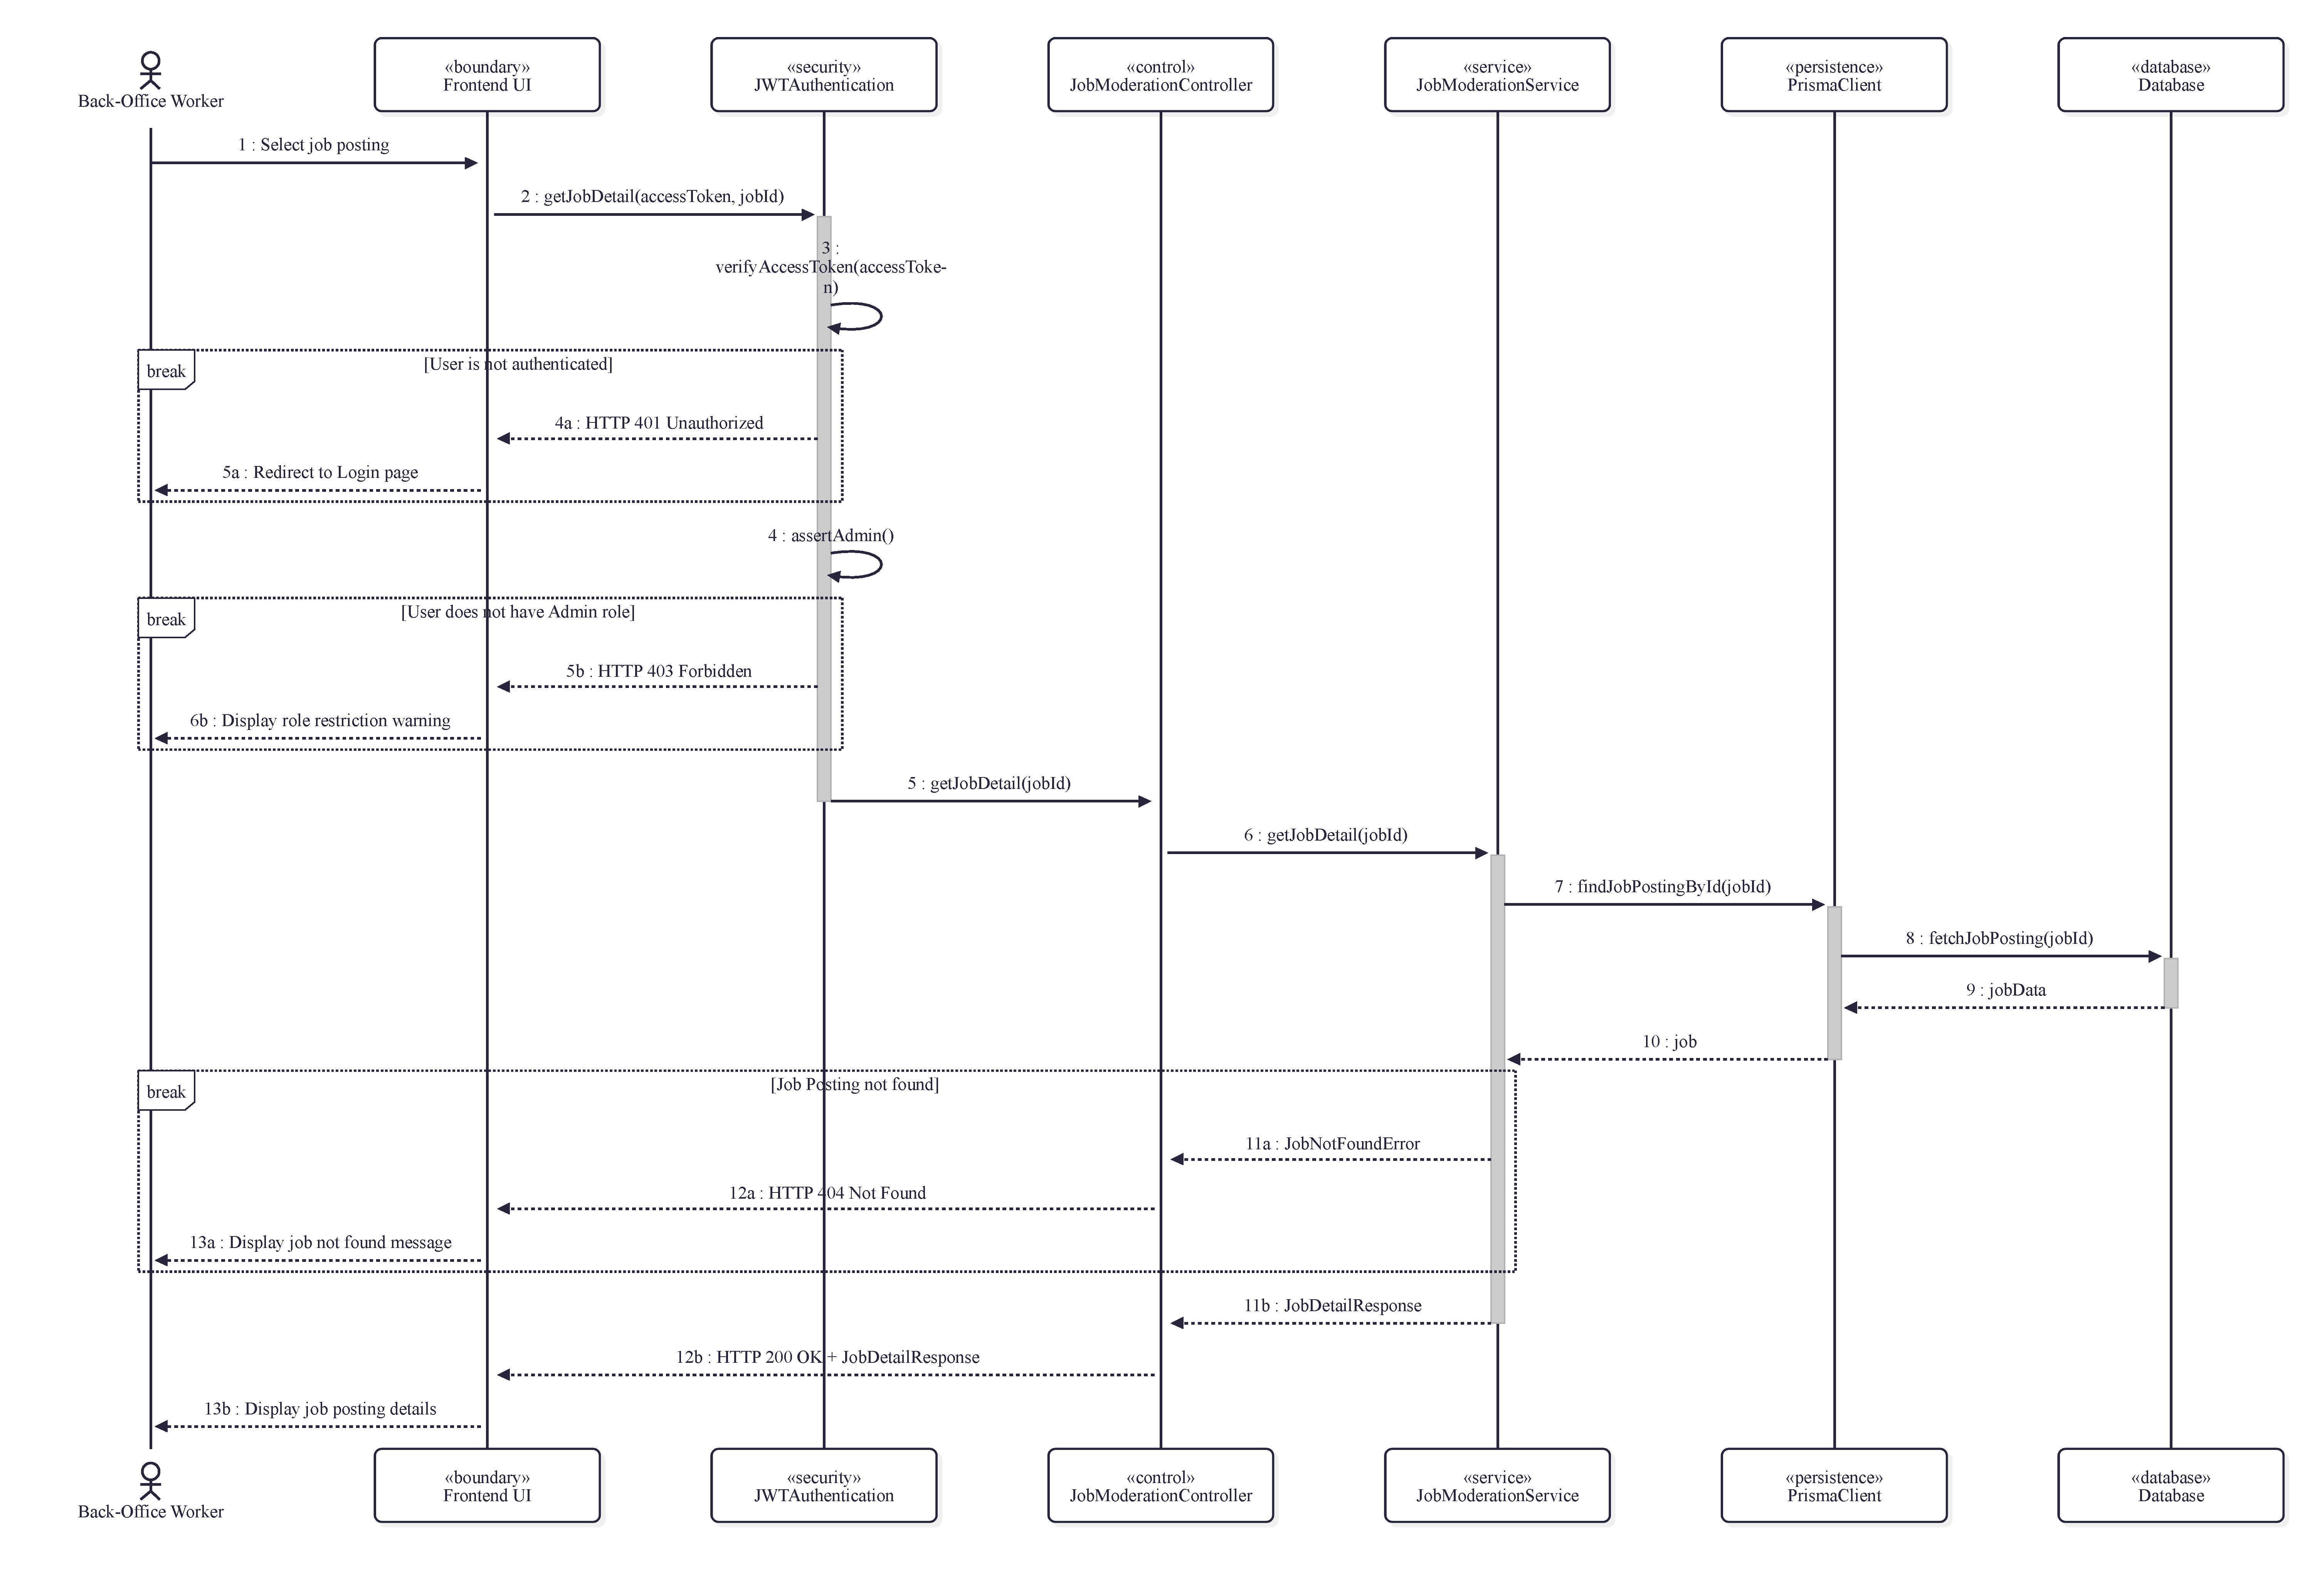
\includegraphics[width=0.9\linewidth]{diagrams/exported/7BackOffice/SD-Admin02-Get-Job-Posting-Detail.pdf}
	\caption{Sequence Diagram: Get Job Posting Detail.}
	\label{diagram:sd-admin-job-detail}
\end{figure}

\begin{figure}[H]
	\centering
	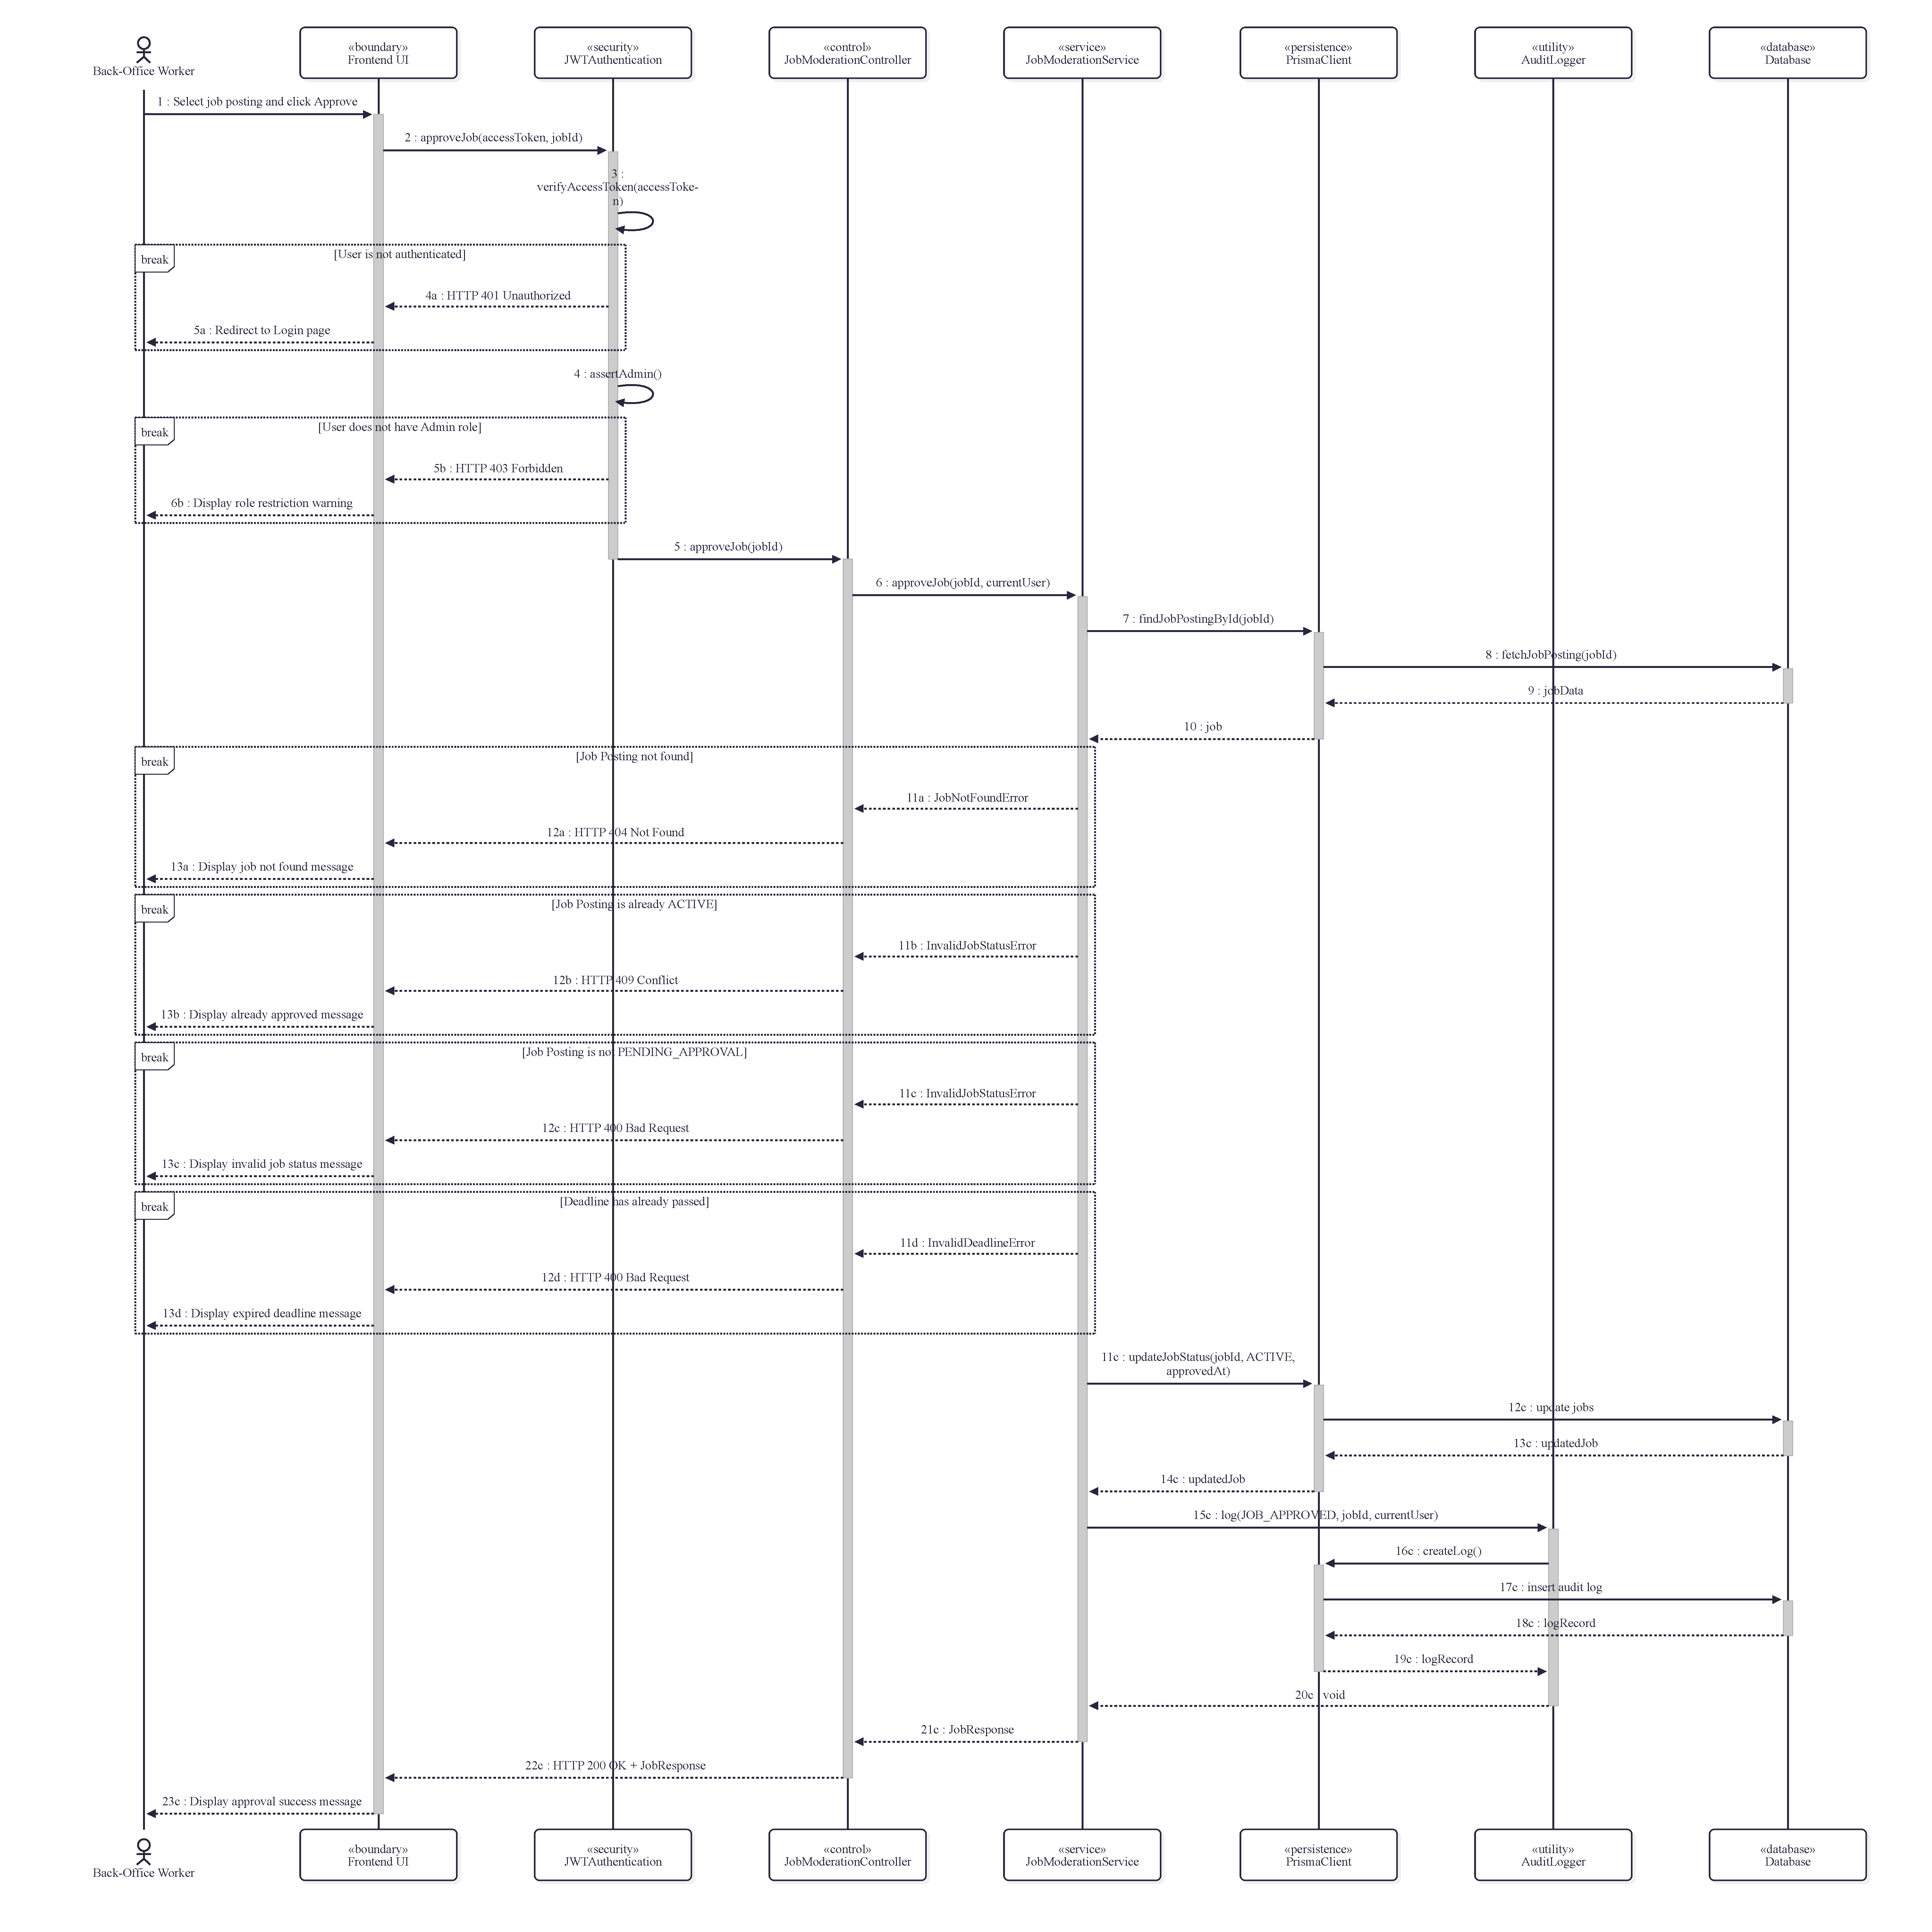
\includegraphics[width=0.9\linewidth]{diagrams/exported/7BackOffice/SD-Admin03-Approve-Job.pdf}
	\caption{Sequence Diagram: Approve Job.}
	\label{diagram:sd-admin-approve}
\end{figure}

\begin{figure}[H]
	\centering
	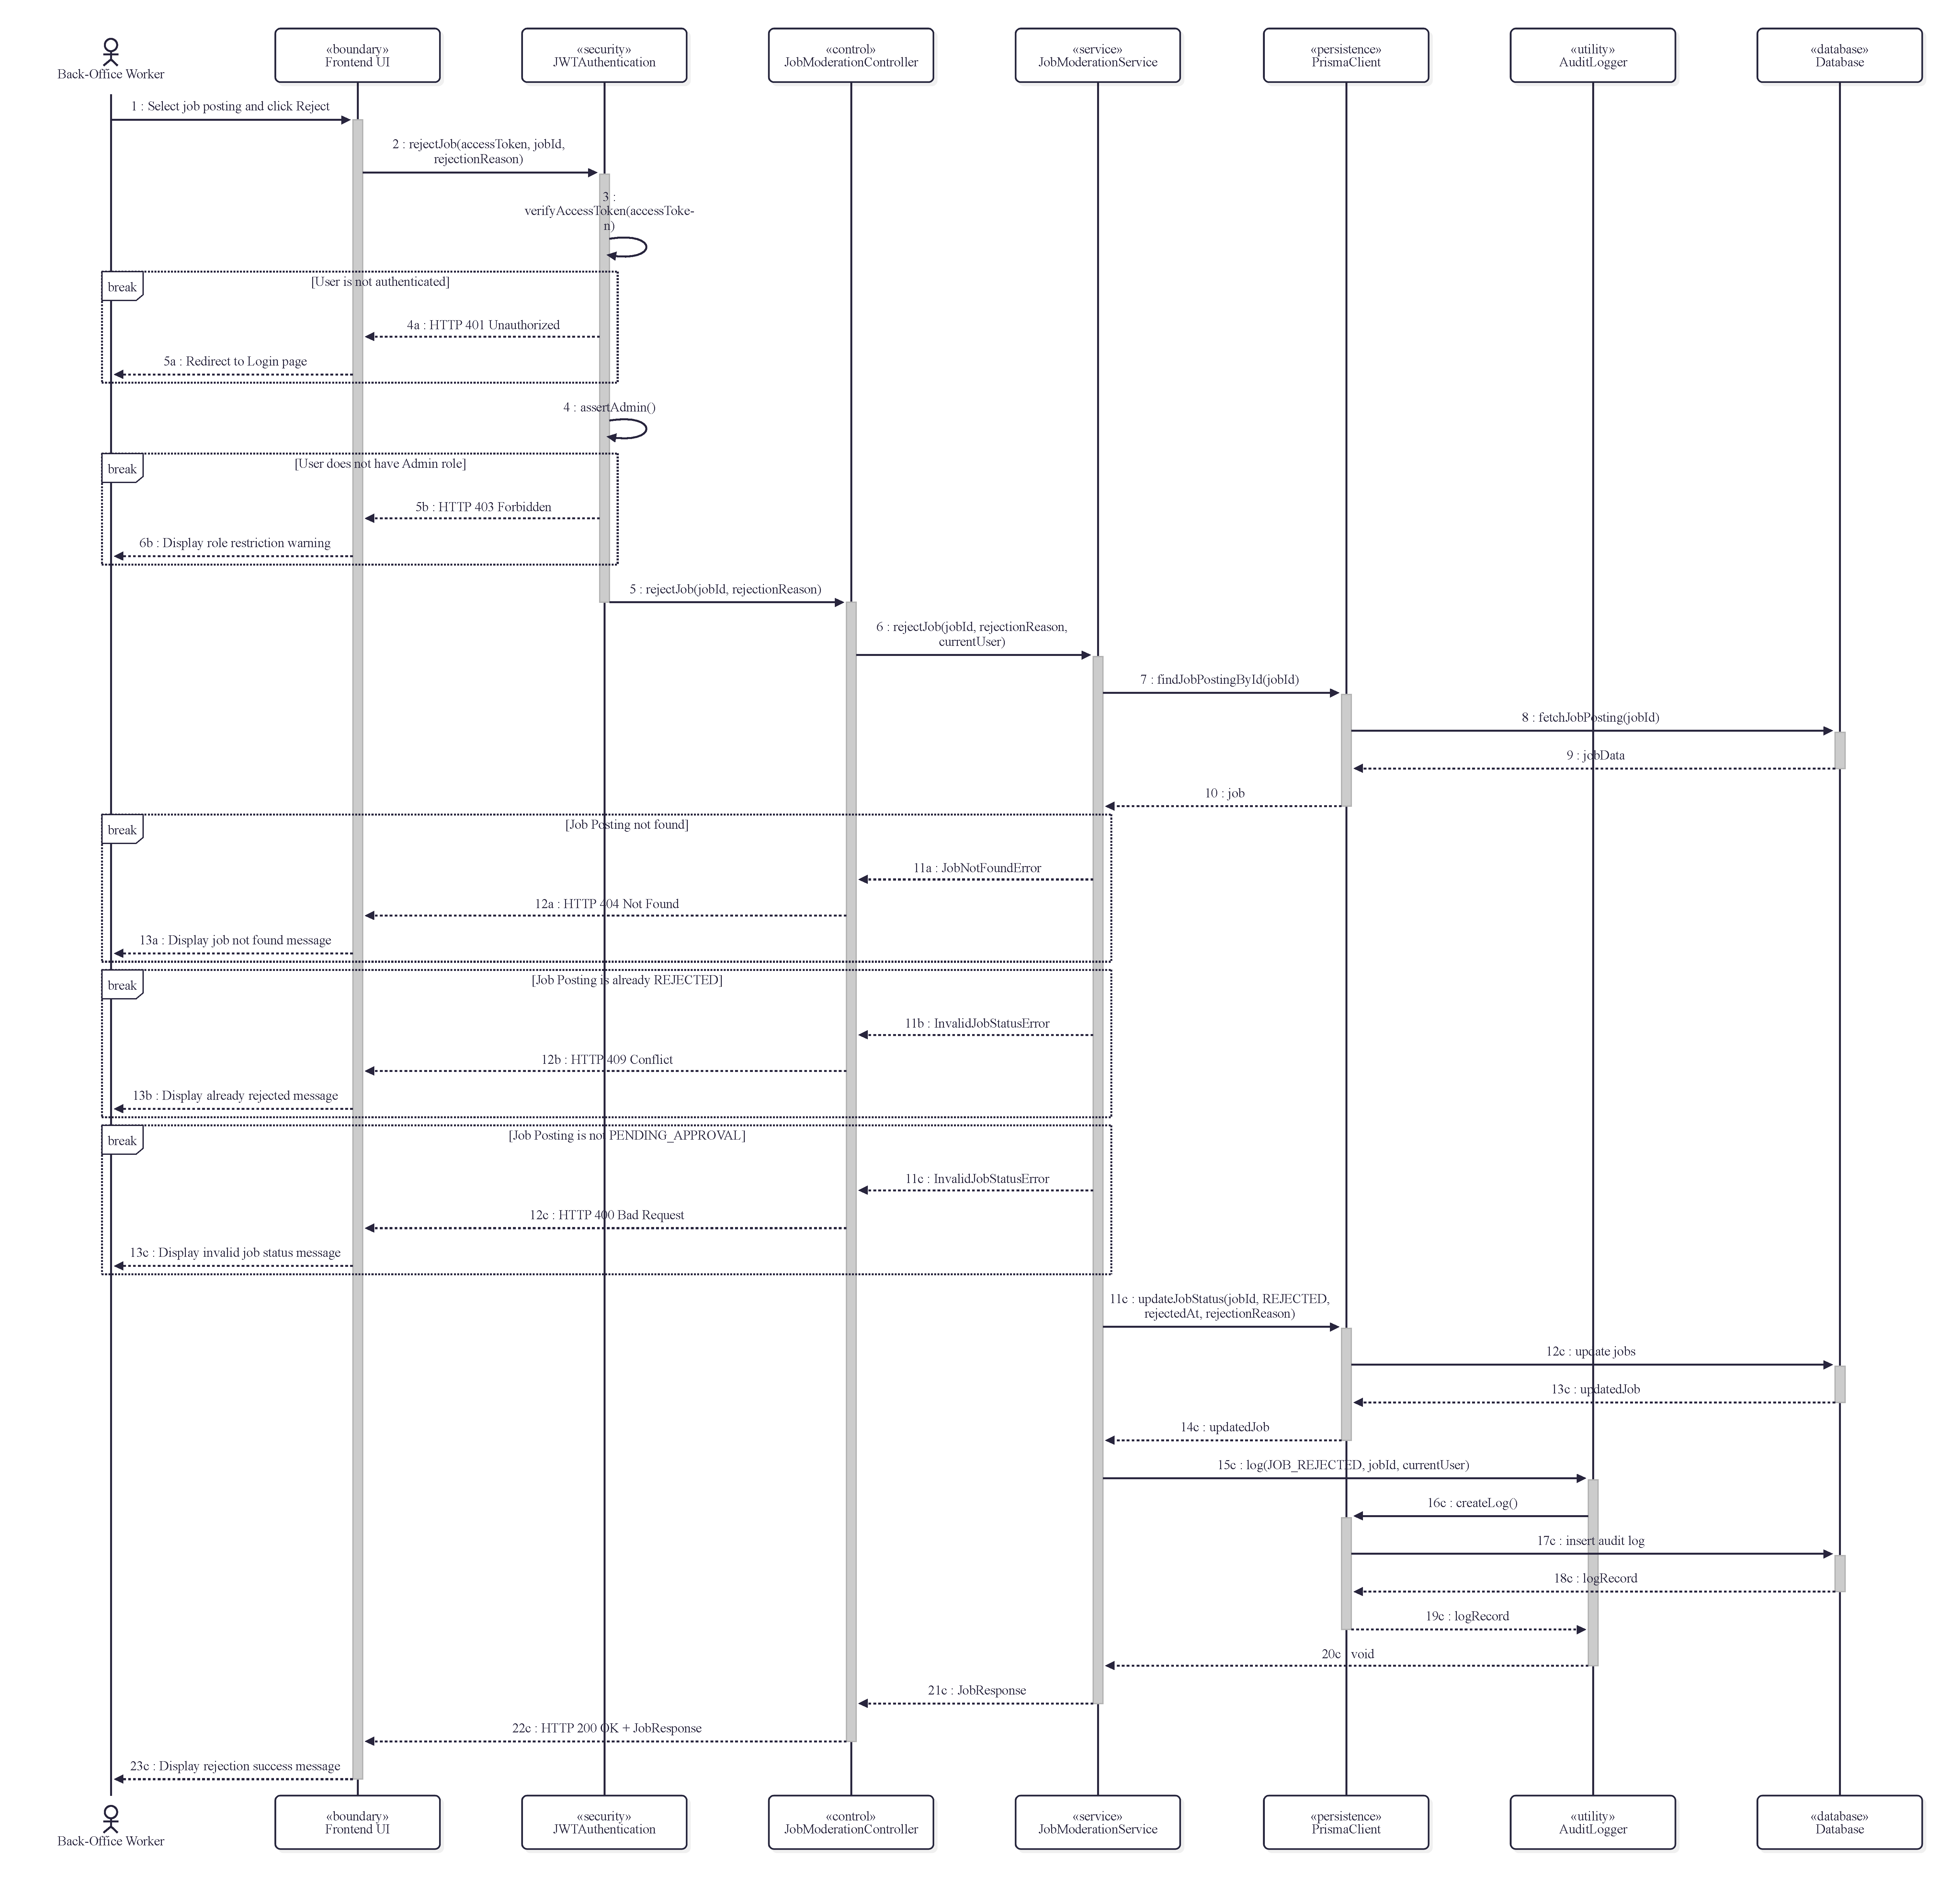
\includegraphics[width=0.9\linewidth]{diagrams/exported/7BackOffice/SD-Admin04-Reject-Job.pdf}
	\caption{Sequence Diagram: Reject Job.}
	\label{diagram:sd-admin-reject}
\end{figure}

\begin{figure}[H]
	\centering
	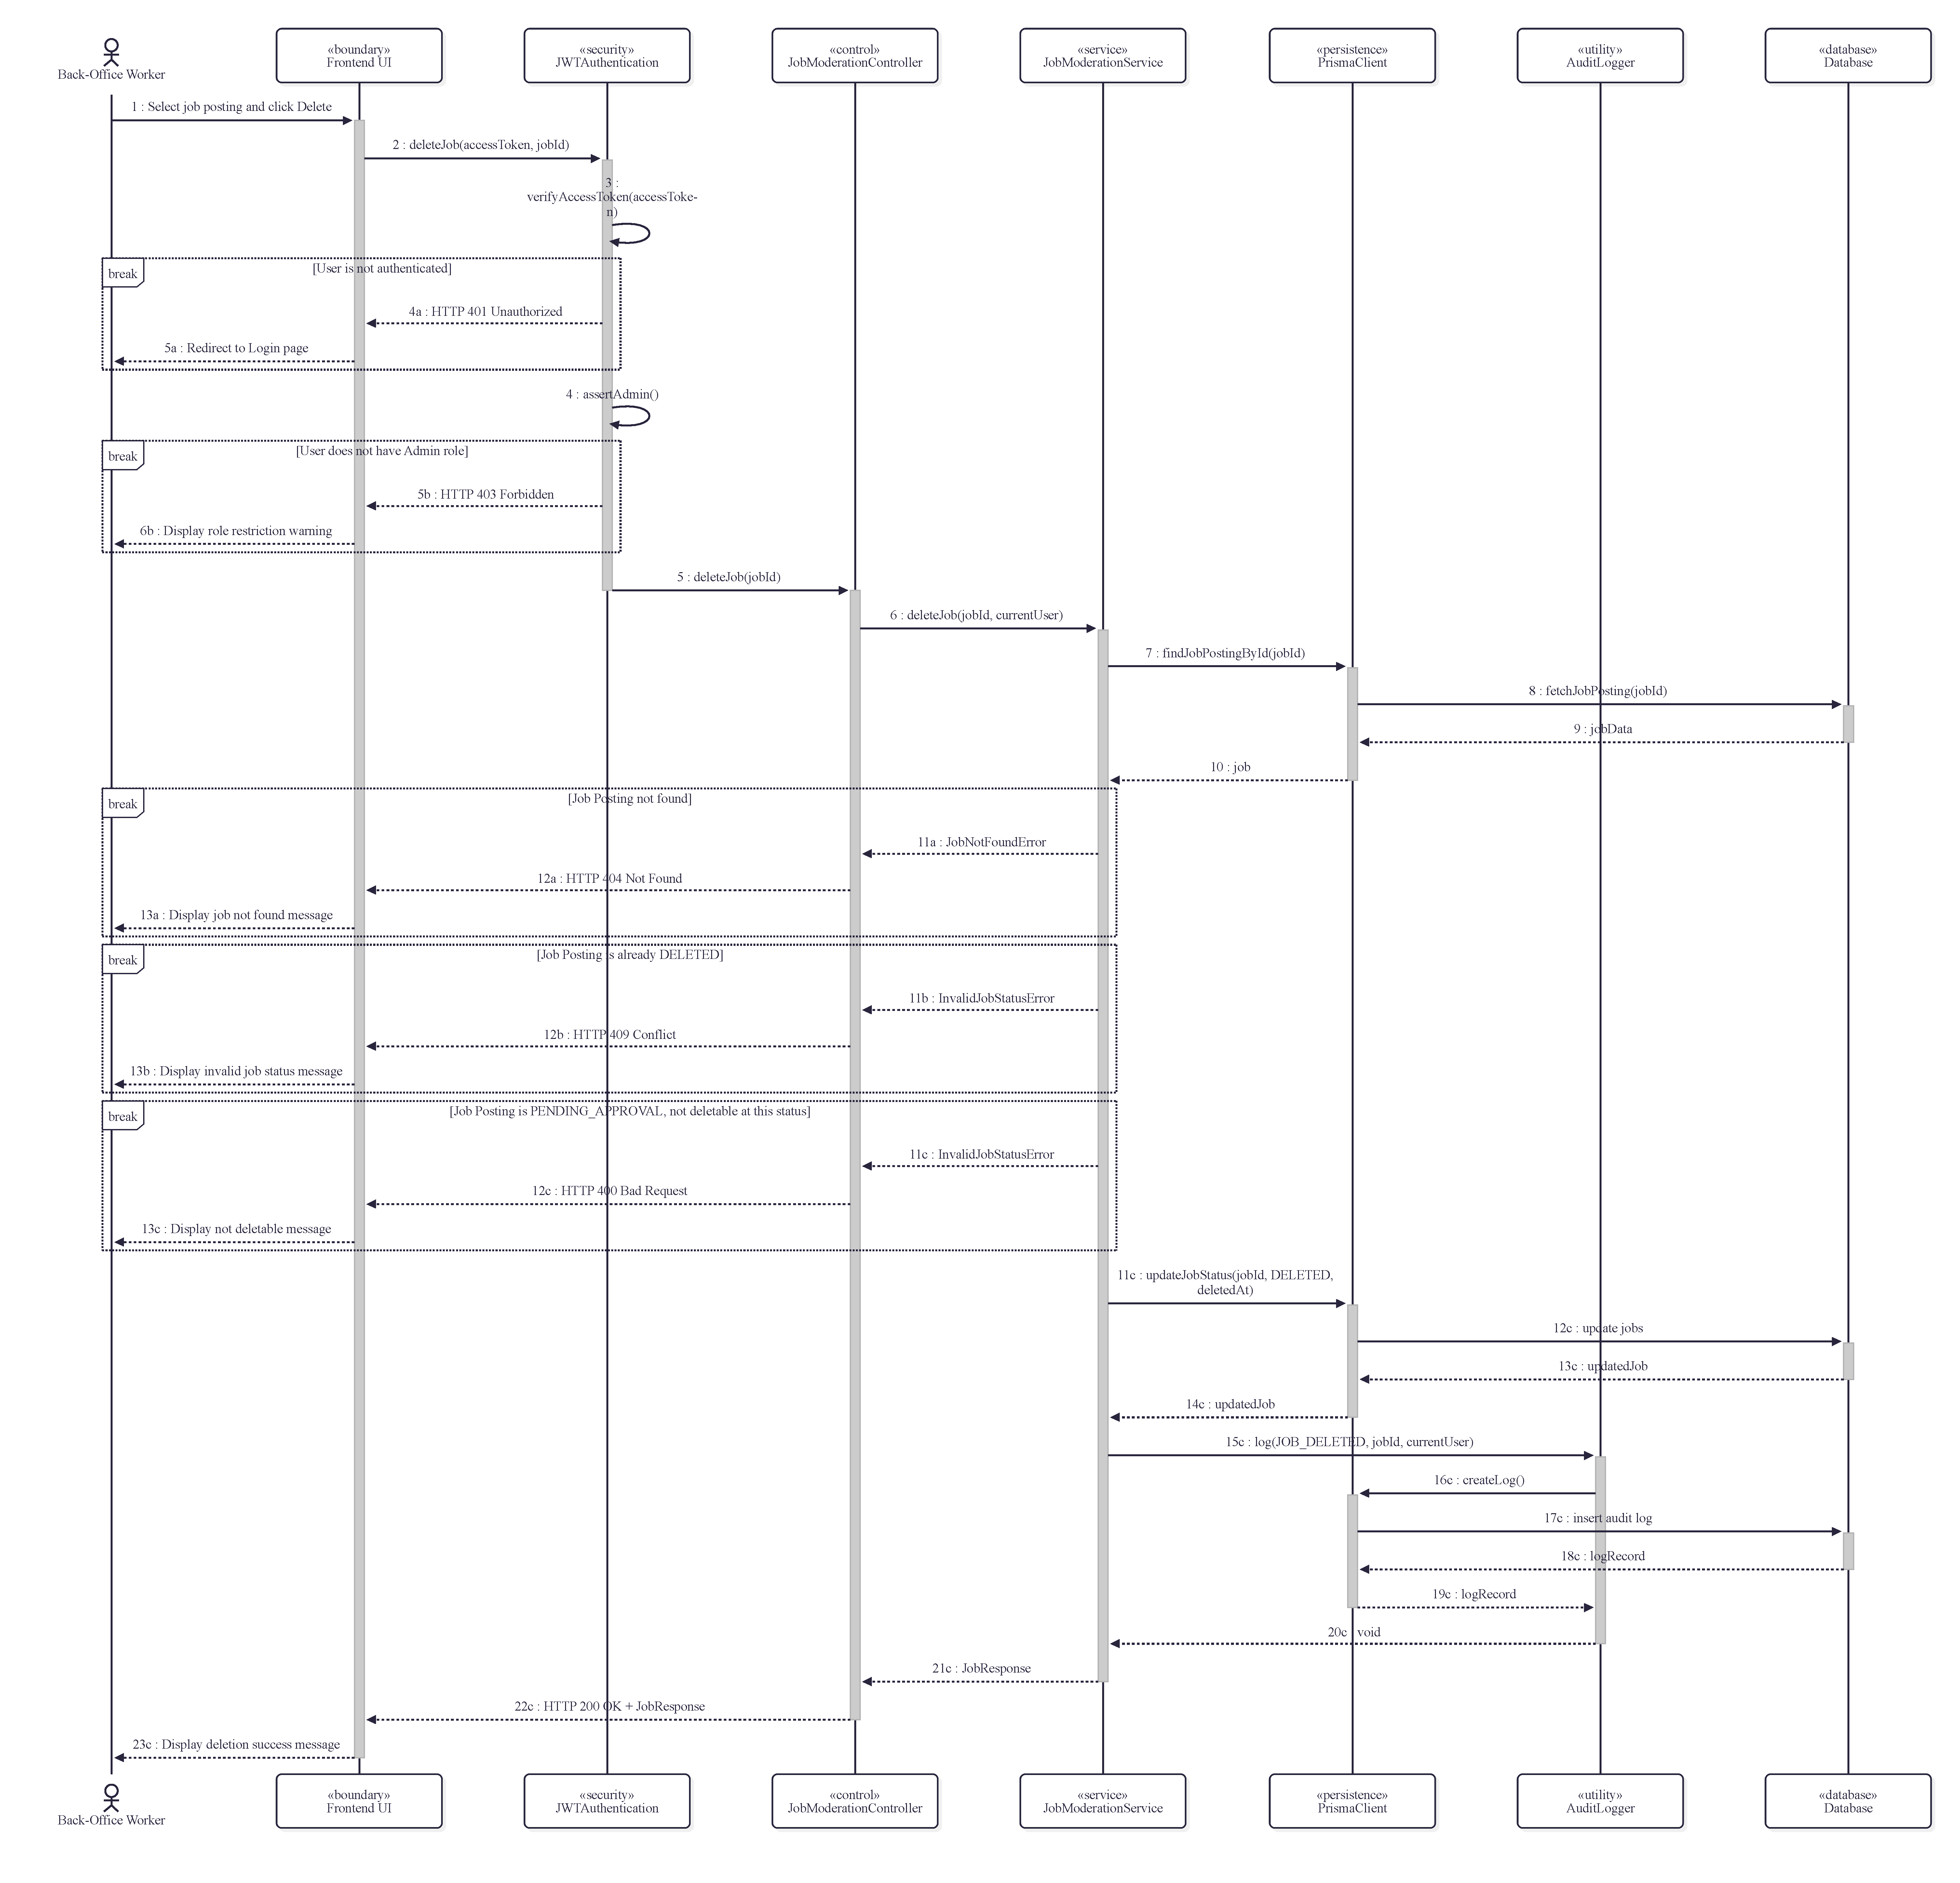
\includegraphics[width=0.9\linewidth]{diagrams/exported/7BackOffice/SD-Admin05-Delete-Job.pdf}
	\caption{Sequence Diagram: Delete Job.}
	\label{diagram:sd-admin-delete}
\end{figure}